\documentclass[usenames,dvipsnames.linkcolor=tudelft-green, citecolor=tudelft-sea-green, urlcolor=tudelft-orange]{dissertation}
\renewcommand{\thefootnote}{\Roman{footnote}}
\usepackage{subcaption} 
\usepackage[english]{babel}
\usepackage{mathrsfs}
\usepackage{amsthm,amsmath,amssymb,amsfonts} 
\usepackage{braket}
\usepackage{multicol}
\renewcommand{\hbar}{\hslash}
\usepackage{fourier}
\usepackage{hyphenat}
\begin{document}

%% Specify the title and author of the thesis. This information will be used on
%% the title page (in title/title.tex) and in the metadata of the final PDF.
\title[]{Green's Function methods for transport calculations involving strong capacitive interactions}
\author{Josko}{de Boer}

%% Use Roman numerals for the page numbers of the title pages and table of
%% contents.
\frontmatter

\begin{titlepage}
 
\begin{center}

%% The following lines repeat the previous page exactly.

\vspace*{2\bigskipamount}

%% Print the title.
{\makeatletter
\titlestyle\bfseries\LARGE\@title
\makeatother}

%% Print the optional subtitle.
{\makeatletter
\ifx\@subtitle\undefined\else
    \bigskip
    \titlefont\titleshape\Large\@subtitle
\fi
\makeatother}

%% Uncomment the following lines to insert a vertically centered picture into
%% the title page.
%\vfill
%\includegraphics{title}
\vfill

%% Apart from the names and dates, the following text is dictated by the
%% promotieregelement.

{\Large\titlefont\bfseries M. Sc. Thesis}

\bigskip
\bigskip



\bigskip
\bigskip

by

\bigskip
\bigskip

%% Print the full name of the author.
\makeatletter
{\Large\titlefont\bfseries\@firstname\ {\titleshape\@lastname}}
\makeatother

\bigskip
\bigskip

.

%% Extra whitespace at the bottom.
\vspace*{2\bigskipamount}

\end{center}

\end{titlepage}



%% The (optional) dedication can be used to thank someone or display a
%% significant quotation.
\dedication{\epigraph{They say a little knowledge is a dangerous thing,

but it's not one half so bad as a lot of ignorance.}{Sir Terry Pratchett}}

\chapter*{Preface}
\setheader{Preface}

Long ago, in 2013, I performed my B.Sc. thesis under Dr. Jos Thijssen. He chose the most educational course, which was to let me make errors. This is, by far, the most effective way to be taught, even if it is not the most effective way to success.

When I asked Dr. Thijssen if he had M.Sc. thesis subjects in 2014, he had a whole list. We settled on this particular subject, which is to take the non-equilibrium Green's Function formalism and add capacitive interactions to it analytically.  This was exciting; it was theoretical work promising publication at some point. Additionally, we would try to explain the measurements made by Mickael Perrin, which were significantly weaker than the theory apparently predicted.

The thesis, I think, succeeded, despite the fact that Dr. Thijssen spent most of his attention on educating other minds, whereas I also had a Ph.D. grant proposal to write. Even so, we looked at a large portion of the parameter fields of our relatively simple model, trying to understand its intricacies. I also found a promising derivation for incorporating phononic interactions.

Of course, Dr. Thijssen does not work alone; conversations with his Ph.D. student, Jose Celis Gil, were very helpful and intriguing. Likewise, I've also spoken to Mickael Perrin and Max Koole several times, which I think greatly helped understanding the experimental side of the story. 

So, I would like to thank my advisor, Dr. Jos Thijssen, his Ph.D. student, Jose Celis Gil. Without their experience, knowledge, guidance and participation this thesis would not have been possible. Additionally, I want to thank Dr. Jos Seldenthuis, whom I have never met but whose work and notes are the very foundation this thesis builds upon.

For mental support and listening to my ramblings, I'd like to thank my family, Maaike Jans (girlfriend), Elske Hottinga (mother), Dick de Boer (father), Roy de Boer (brother), Rick de Boer (brother). Also several of my friends, Elizabeth Berghuijs, Jacob Verhaart, Bram van der Veen, Marije Barel and Esmeralda Tomas\"oa.


\begin{flushright}
{\makeatletter\itshape
    \@firstname\ \@lastname \\
    Delft, \today
\makeatother}
\end{flushright}



\tableofcontents

%% Use Arabic numerals for the page numbers of the chapters.
\mainmatter

%% Turn on thumb indices.
\thumbtrue

\chapter{Introduction}
\label{ch:chapter_1}
 
\epigraph{
    “Did I mention that I know almost everything about almost everything ?”
}{Dr. Rodney McKay, fictional character}

\begin{abstract}
Molecular electronics is a relatively young field that attempts to find functional molecular junctions, initially as an alternative to semiconductor devices reaching atomic limits. In this chapter, I sketch both the experimental and theoretical context in which this thesis is placed.
\end{abstract}

%% Start the actual chapter on a new page.
\newpage
\section{Molecular Electronics}
Modern electronics is almost entirely based on semiconductor physics. The most abundant and thus primary element for electronics is silicon. Since the 1960, efforts have been made to minimise the semiconductor devices to ever smaller scales. However, semiconductors are bulk materials, implying a fundamental limit to their minimisation. Now that the downsizing approaches molecular scales, it is at its end ~\cite{seldenthuis}.

The next smallest functional element is a molecule. Evolution by natural selection has, at the biochemical scale, led to a very broad spectrum of functional molecules. A great amount of molecules can be synthesised by utilising the specialised enzymes provided in that way.

At the molecular scale, new functionality also arises. For instance, molecules can respond to light and heat. They can act as logic gates, rectifiers, solar cells and much more ~\cite{perrin}. Experts see the most exciting future of the field in that direction, in new functional elements rather than replacement of semiconductor elements ~\cite{visions}.

Fundamental to the creation of molecular devices is the understanding of their fabrication and behaviour . My thesis focuses almost entirely on the latter aspect, although previous experiments will be discussed as a way of confirming or motivating theoretical work.

It is useful to be aware of some experimental issues. For instance, the contacting of a single-molecule in a device is non-reproducible . Statistical approaches to measure conductance and other molecular properties are essential. The challenge lies partially in reducing the variability or to exploit molecular functionalities that are insensitive to the details of the contacts ~\cite{visions}.

For theory, on the other hand, the challenge lies in removing the mismatch between theory and experiment. In particular, predicting transport gaps and determining location of (frontier) orbital levels with respect to the Fermi energy have proven very challenging~\cite{perrin}. Primarily I focus on incorporating interactions into the formalism. Normally, only single-electron transport is considered, partially because the appropriate formalism  was not available. Starting from a note by Dr. Jos Seldenthuis, I develop the appropriate formalism. I apply this to a model, thereby incorporating Coulomb interactions, that has been shown to qualitatively work well to explain the behaviour of thiolated arelythynylene with a dihydroanthracene core ~\cite{perrinnano}. I also consider a similar model that incorporates spin, although its novelty originates in that it is now imperative to consider it because of interactive effects where it was originally a trivial spin-splitting. 
%%%%%%%%%%%%%%%%%%%%%%%%%%%%%%%%%%%%%%%%%%%%%%%%%%%%%%%%%%%%%%%%%%%%%%%%%%%%%%%%%%%%%%%%%%%%%%%%%%%%%%%%%%%%%%%%%%%%%%%%%%%%%%%%%
\section{Experimental}
I will shortly review a number of the more popular techniques for single-molecule experiments. To wit, these are Conductive Atomic Force Microscopy (C-AFM), Scanneling Tunneling Microscopy (STM), Electromigration and finally Mechanically Controlled Break Junctions (MCBJ). I think it important to have some knowledge of the experimental reality of the nanoscopic devices I investigate theoretically.

Atomic Force Microscopy is a type of scanning probe microscopy with resolution of less than a single nanometre. By using a piezoelectric element, it can make an accurate surface scan by keeping the forces between probe and sample constant~\cite{frei1, frei2}.

For molecular electronics, molecules are evaporated onto the gold substrate. The AFM tip, a golden cantilever, is brought into contact with a substrate and slowly retracted. The evaporated molecules form a self-assembled mono layer, so that some molecules have migrated onto the substrate-tip bond. As it breaks, a molecular break junction is formed. However, this requires conductive molecules, which is why the technique is referred to as Conductive-AFM (C-AFM). Also, it is relevant that usually C-AFM measurements concern groups of molecules, only rarely a single molecule.

The AFM method has several features. First, it can measure both electrical current and forces in a parallel measurement~\cite{nef}. Another large advantage is that the topographic imaging and electrical measurement are simultaneously achieved, so that the nano-device is relatively well documented before measurement ensues.

The Scanneling Tunneling Microscopy method features similar advantages \cite{Joachim2000}, but instead of using a golden cantilever it is the scanning probe tip that is brought into contact with a molecule, and then very slowly pulled away. The molecule, which bonds to the tip, is the stretched between the substrate and the STM tip, making another (gold) molecular junction.

Electromigration is a method of gap formation that makes use of increased mobility due to the application of voltage. An overlapping set of gold leads is made, which is subject to voltage ramps at ambient laboratory conditions. The voltages increase the mobility of the gold atoms, which move away from the future gap. The gap formed by this method is highly irreproducible~\cite{electromigration}.

Finally, the Molecular Controlled Break Junction is the technique used by~\citet{perrinnano}, whose work I will discuss later in section~\ref{sec:perrin}. In figure~\ref{fig:mcbj} the basic setup of a Mechanically Controllable Break Junction (MCBJ) is shown~\citet{perrin} . These offer high electrode stability and fine-tuning of the electrode spacing. 
\begin{figure}[!bp]
    \centering
    \includegraphics[height=0.3\textheight,page=2, clip=true, trim=2.5cm 16.5cm 11cm 6cm]{pdf/perrinnnano.pdf}
    \caption{Schematic drawing of a MCBJ. A Gold wire is deposited on top of a flexible substrate, which is then bend by the three-point mechanism. The wire breaks, forming a size-controllable gap.}
    \label{fig:mcbj}
\end{figure}

The working principle behind the MCBJ technique is to deposit a thin metallic wire on top of a flexible substrate. Gold is often used because it is a noble metal. By bending the substrate in a three-point mechanism, the gold wire stretches and breaks. It then forms two gold surfaces, the electrodes. The spacing between these electrodes can be tuned by adjusting the bending of the sample. The junction can be reformed after it is broken.

The allowed voltage over such a MCBJ junction ranges from $0.5$ V at room temperature up to $2$-$3$ V at $4.2$K. At low temperatures, the size of the gap does not significantly change over time. Additionally, the technique allows repeated fusing and breaking, and is thus ideal for statistical studies which are required for mechanistic insight because of the large fluctuations in experiments \cite{ratnerrev2013}.

A few examples of experimental findings~\cite{koole} involving molecular electronics are the Coulomb blockade~\cite{Park2000, Park2002}, the Kondo effect~\cite{Park2002}, vibrational excitations~\cite{vib1, vib2} and electronic excitations~\cite{elec1}.

\section{Theory}
\label{sec:theoryintro}
While I work primarily in the non-equilibrium Green's Function Formalism (chapter~\ref{ch:chapter_2}), here I will also briefly describe another formalism often used, namely the Master Equation approach \cite{seldenthuis}. One very large benefit of the Master Equation approach over the non-equilibrium Green's Function approach is that it has a simple conceptual interpretation.

Let us start by noting that molecules can be viewed as a collection of quantum dots. For instance, consider a simple chain of carbon atoms, with transport dominated by a single atomic orbital. It makes sense that one can describe this chain with the simplified model of a chain of quantum dots with a single energy level for each individual dot, thereby leading to 4 orbital levels of the molecule. If spin is included, the system could even be described as a chain of Qubits.

The typical way of physicist thinking is the Master Equation (ME) approach. The ME approach is only valid for weak coupling, so it is technically not relevant for a chain of carbon atoms. However, the chain of carbon atoms was only a parable with the aim of establishing the collection of quantum dots picture.

If one considers one of these dots centred between two others ($c$) , then one needs to know the rate $W$ at which electrons leave it to either the right ($r$ or the left ($l$) neighbouring dot, and the rate at which they enter. Of course, the net flux depends on the chances $P$ the neighbouring dots are occupied. For instance, the flux of electrons coming from the left is the chance that the left dot is occupied $P_l$ times the rate $W_{l\rightarrow c}$ of electrons moving from the left ot the central dot. Based on this simple reasoning, I formulate the Master Equation \cite{beenakker}:
\begin{align*}
\partial_t P_c &= P_l W_{l\rightarrow c} - P_c W_{c\rightarrow l} + P_r  W_{r\rightarrow c} - P_c W_{c\rightarrow r}
\end{align*}

Of course, I do not yet know the rates of leaving and entering the central dot. However, note that the master equation is linear and can be written in matrix form, $\dot{P} = W P$. For a more elaborate system, the system would have multiple states on each dot, and fluxes would look like e.g. $P_{li} W_{li\rightarrow cj}$, denoting the flux of electrons that occupied the left dot in a numbered state $i$ to the central dot in state $j$.  

Any molecule has as constituents the atoms and the electrons. Generally the atomic background of the electrons is approximated as an effective potential. However, it is known that molecules can have nuclear motion, which can feature in transport as well, e.g. phonon interactions or vibrational modes. I therefore use the Born-Oppenheimer approach (section~\ref{sec:schrodinger}), where it is assumed the wave-function $\ket{\Psi}$ is separable into the atomic nuclei state $\ket{\phi}$ and the electronic state $\ket{\psi}$. The rates due to a (weak) interaction $H'$ be found from the well-known Fermi's Golden rule between initial state $\ket{i}$ and final state $\ket{f}$:
\begin{align*}
W_{i\rightarrow f}  &= \frac{2\pi}{\hbar} \left| \braket{\Psi_f \left|H'\right| \Psi_i}\right|^2 \rho_f (\epsilon_f)  \\
&= \frac{2\pi}{\hbar} \left| \braket{\phi_f \psi_f \left|H'\right| \phi_i \psi_i}\right|^2 \rho_f (\epsilon_f),
\end{align*}
where $\rho_f(\epsilon_f)$ denotes the final density of states. 

The atomic overlap $\left| \braket{ \phi_f | \phi_i }\right|^2$ is known as a Franck-Condon factor (section~\ref{sec:phononic}). Note that different electronic eigenstates very often have a slightly different atomic state, which means that the Franck-Condon factor between non-identical states become non-zero. Theoretically, this can be understood as a basis change; $\ket{\phi_i}$ and $\ket{\phi_f}$ are no longer pure eigenstates in the new basis. 

The ME approach is very suited to handling vibrational excitations and interactions up to any desired order \cite{seldenthuis}. However, it only describes systems where electronic interactions are weak. The non-equilibrium Green's Formalism (chapter~\ref{ch:chapter_2}) is its opposite, and is more suited to strong electronic interactions, such as tunneling or Coulomb interaction. 

One particular feature is that the ME approach assumes that electrons remain on a `dot' for long times, losing all phase information. Therefore, quantum interference is a feature that the ME approach does not cover, thereby requiring that the level spacing is larger than the effective coupling $\delta \epsilon_i \gg \Gamma$.

Both the ME approach and the NEGF formalism deal with molecules; small functional blocks. However, you need to characterise the molecule or at the very least its single-electron orbitals at the HOMO and LUMO level. 

I will now describe Density Functional Theory (DFT) as it pertains to transport calculations for single-molecule junctions. This theory is very well known and recognised, as is evident by the 1998 Nobel Prize in Chemistry, shared equally between Walter Kohn "for his development of the density-functional theory" and John A. Pople "for his development of computational methods in quantum chemistry"~\cite{nobel1998}. 

The starting point for DFT is that the ground-state density $n(r^\mu)$ for any electronic system uniquely determines the system, even if interacting\footnote{I denote the positions of atoms as $r^\mu = (x,y,z)$.}. Effective approximations for the functionals involved in DFT lead to the DFT calculations of today (e.g. LDA, GGA). 

Let us describe, briefly, the general approach of DFT. DFT starts with some initial guess $n^0(r^\mu)$. Using this guess, the general DFT approach constructs a Schr\"odinger equation which depends on the electron density rather than the individual electron orbitals\cite{joscomp}. Solving this Schr\"odinger equation leads to a new density, $n^1(r^\mu)$, which is then used to construct a new Schr\"odinger equation. This iterative self-consistency loop is broken when the electron density converges.

As a specific DFT example, the Kohn-Sham approach minimises the single-particle Kohn-Sham equations \cite{kohnsham, joscomp}:
\begin{align}
\left( -\frac{1}{2} \nabla^2 + v_\text{eff} (r^\mu) - \epsilon_i \right) \varphi_j( r^\mu) &= 0, \label{eq:ks}
\end{align}
with
\begin{align*}
n(r^\mu) &= \sum_{j=1}^N \left| \varphi_j (r^\mu)\right|^2,\\
v_\text{eff} &= v(r) + \int \frac{n(x^\mu)}{\left|r^\mu - x^\mu\right|} dx^\mu + v_\text{xc}(r^\mu),
\end{align*}
where $v_\text{xc}(r^\mu)$ is the local exchange-correlation potential, a chosen functional that depends on the density distribution $n(r^\mu)$ of the current iteration.


I have now described the basic process of a DFT calculation. Depending on the implementation, a basis set might have to be chosen in addition to the exchange-\-correlation functional.The DFT calculation returns the Hamiltonian of the system on the chosen basis. To this Hamiltonian the non-equilibrium Green's Function Formalism (chapter~\ref{ch:chapter_2})can be applied, although it exists independently. I will discuss this formalism at length for both arbitrary and model Hamiltonians.

\section{Outline of thesis}
In this M.Sc. Thesis, the focus lies on interactions in the non-equilibrium Green's function formalism, specifically capacitive interactions. The Coulomb interaction is capacitive, allowing me to incorporate it into the NEGF formalism.

First, in chapter~\ref{ch:chapter_2} I derive the non-equilibrium Green's Function formalism from first principles for a generic Hamiltonian $H$. Next, I consider the derivation that incorporates interactions in chapter~\ref{ch:chapter_3}. The first and most important result of this thesis are the capacitive interactions of section~\ref{sec:capacitive}, but I will also took a brief look at vibrational excitations.

I then apply the new theory  in chapter~\ref{ch:chapter_4}. Specifically, I apply it on the two site model Hamiltonian used in \citet{perrinnano} and discuss the results. Finally, in chapter~\ref{ch:chapter_5} I discuss the findings and implications of the new theory. I also summarise the thesis and make suggestions for future research.

%clearpage dumps all images in the stack. Also prevents images from skipping chapters.
\clearpage
\references{dissertation}
\chapter{Approach: The non-equilibrium Green's Function formalism}
\label{ch:chapter_2}

%% The following annotation is customary for chapter which have already been
%% published as a paper.
%\blfootnote{Parts of this chapter have been published in Annalen der Physik \textbf{324}, 289 (1906) \cite{Einstein1906}.}

%% It is only necessary to list the authors if multiple people contributed
%% significantly to the chapter.
%\authors{Albert {\titleshape Einstein}}

%% The '0pt' option ensures that no extra vertical space follows this epigraph,
%% since there is another epigraph after it.
%\epigraph[0pt]{
%    "quote1"
%}{attribution}

\epigraph{
    “A rock has no detectable opinion about gravity.”
}{Sir Terry Pratchett}

\begin{abstract}
In this section, I fully derive the non-equilibrium Green's Function Formalism, the Dyson and Keldysh Equations, and several other useful quantities. We will look explicitly at properties of interest, such as the occupation of the levels of and the current through the molecule.
\end{abstract}

%% Start the actual chapter on a new page.
\newpage
\section{Introduction}
Any quantum mechanical system can in principle be described by the Schr\"odinger equation. For a system with a finite number of particles, there are several methods for solving the many-body Sch\"odinger equation, for instance the popular Hartree-Fock (HF) and density-functional theory (DFT) quantum chemistry methods.

However, no laboratory system is a finite system. A molecule is coupled to metallic electrodes, which connect to a voltage source. The circuit is further extended with measurement equipment, refrigeration instruments and so forth. The system might also not be in equilibrium, such as when a bias voltage is applied between the two electrodes. In this situation, solving the Schr\"odinger equation directly is unfeasible \cite{seldenthuis}.

Green's functions are a familiar concept in partial differential equations. Here, Green's functions characterise a partial differential equation completely, allowing you to solve for any given initial and boundary conditions and possible forcing terms rather easily by integration. For instance, the Green's function for the Heat Equation $G(x,t; x_0, t_0)$ expresses the influence of the temperature at $(t_0, x_0)$ on the temperature at $(t,x)$ \cite{haberman}. 
While I will try to give a self-inclusive derivation of the non-equilibrium Green's Function (NEGF) formalism, I refer the reader to Refs.~\cite{mattuck,diventra,haugjauho} for a more complete overview.

For a closed system in equilibrium, the GF formalism is exact because it is simply a rephrasing of the Schr\"odinger equation. However, the NEGF method also provides a systematic approach to incorporate some non-equilibrium interactions of nanoscopic systems with infinitely large environments.

It is perhaps illuminating to first go over a number of assumptions and approximations \cite{seldenthuis}. 

First, the metallic electrodes or leads are considered as infinite reservoirs that are non-interacting and are in equilibrium and not influenced by the molecule. Note that the leads are not required to be in equilibrium with each other. Although the immediate environment of the molecule is likely to be influenced by the molecule, it is possible to partition the system as you desire. The Extended molecule that also includes the lead-tip thus solves the problem of molecule-lead influence.

Second, there is an assumption of adiabatic temporal evolution, so that the system in the infinite past can be considered as isolated leads and molecule.  

Finally, the system is an open quantum system. Electrons travel to the leads and move into an infinite reservoir, thus losing all information of their dynamics. 

These tree approximations or assumptions are sufficient to obtain closed expressions for the properties of interest. However, as usual the equations become unwieldy for systems that approach the complexity of an actual laboratory nanoscopic system, requiring ridiculous computational resources.

It is for this reason that other approximations are employed for practical application, such as the mean-field approximation. In this approximations the interactions are essentially averaged out, which makes \emph{ab initio} quantum transport problems tractable. However, you lose certain transport phenomena, most notably the \emph{Coloumb Blockade} (section~\ref{sec:capacitive}).

This chapter is outlined as follows. First, I will consider the unwieldy many-body Schr\"odinger equation in section~\ref{sec:schrodinger}. We will then introduce Slater determinants and move on to the Fock-space and the formalism of second quantisation in section~\ref{sec:secondquantisation}. 

I will then derive the application of the Green's Functions in section~\ref{sec:greensfunctions}. How to find them will be discussed in section~\ref{sec:eommethod}.

Finally, I discuss how to find properties of interest in section~\ref{sec:properties} and the common application of the formalism in section~\ref{sec:synthesis}.

\section{Many Body Schr\"odinger Equation}
\label{sec:schrodinger}

For an arbitrary number $N$ of particles, both electrons and others, the many-body Schr\"odinger equation is:
\begin{align}
 \imath \hbar \partial_t\ket{\Psi\left(t, r_0, r_1, \ldots r_N\right)} &= \widehat{H} \ket{\Psi\left(t, r_0, r_1, \ldots r_N\right)} \label{eq:schrodinger}, \\
 H &\equiv V\left(t, r_0, r_1, \ldots r_N\right) - \sum_{i=0}^N \frac{\hbar^2}{2m_i} \nabla_i^2
\end{align}

It is clear that for many-particles ($N\gg 1$), equation~\ref{eq:schrodinger} becomes unwieldy rather rapidly. We will need some approximations before it becomes applicable.

If we consider the Hilbert space of Atoms $H_A$ and that of electrons $H_e$, then their composite Hilbert space is $H = H_A \otimes H_e$. If the basis of $H_A$ is $\ket{\phi_i}$ and that of $H_e$ is $\ket{\psi_j}$, then an arbitrary state is:
\begin{align}
\ket{\Psi} &= \sum_{ij} c_{ij} \ket{\phi_i} \otimes \ket{\phi_j}
\end{align}

Such a state is separable if there exists vectors in the atomic space $\ket{\Psi_A}$ and in the electron space $\ket{\Psi_e}$ such that $\ket{\Psi} = \ket{\Psi_A} \ket{\Psi_e}$. An alternative formulation is that states that are separable are not entangled.

The Borne-Oppenheimer approximation is that the electron and atom  states are separable \cite{mattuck}. It is justified because atoms are about three orders of magnitude more massive than electrons, and as such they are expected to move much more slowly. The convenience of the Borne-Oppenheimer approximation is that the effect of the atoms, i.e. that of the molecular skeleton, is to provide an effective background potential for the electronic wave functions.

The Hamiltonian then reduces to the following effective electron-only form:
\begin{align}
H_e &= \sum \frac{p^2}{2m} + V_A + H',
\end{align}
where $V_A$ is the effective atomic background potential and $H'$ simply describes the interactions.

\section{Second Quantisation}
\label{sec:secondquantisation}
If we consider a single-particle (fermion) basis $H_{sp}$ with the wave function or states of the $i$-th particle at momentum $k_j$ denoted $\ket{\phi_{k_j}(r_i)}$\footnote{Here and elsewhere, I do not literally write down the spin of a state. Consider it understood that spin is included in the labelling of the states, i.e. $k \rightarrow \sigma, k$.}, with the full electron Hilbert space the successive tensor products $H_{e} = H_{sp} \otimes H_{sp} \otimes \ldots \otimes H_{sp}$ the separable single-particle wave function products still span the space $H_e$. However, the symmetry requirements of the Pauli exclusion principle have to be satisfied, leading to the Slater determinant\cite{yuli}:
\begin{align}
\ket{\Phi_k} &= \frac{1}{\sqrt{N!}} \begin{vmatrix}
\ket{\phi_{k_0}(r_0)} & \ket{\phi_{k_0}(r_1)} &\ldots& \ket{\phi_{k_0}(r_N)} \\
\ket{\phi_{k_1}(r_0)} & \ket{\phi_{k_1}(r_1)} &\ldots& \ket{\phi_{k_1}(r_N)} \\
\ldots&\ldots&\ldots&\ldots&\\
\ket{\phi_{k_N}(r_0)} & \ket{\phi_{k_N}(r_1)} &\ldots& \ket{\phi_{k_N}(r_N)} \\
\end{vmatrix},
\label{eq:slaterdeterminant}
\end{align}
which describes a full state under the requirement of a specific momentum. Note that the matrix must be $N\times N$. If there are less states than particles, the Pauli exclusion principle cannot be satisfied. If there are more states than particles, then some are simply not occupied and shouldn't be in the product.

That leads us to the notion of a Fock state. A Fock state fully specifies a quantum many-body state by essentially listing the occupied states. However, it does not tell you which particle is in what state, which fits the Slater determinant splendidly:
\begin{align}
\ket{\Phi_k} &= \ket{n_{k_0}, n_{k_1},\ldots, n_{k_M}},
\label{eq:fock}
\end{align}
where $M$ simply is the total number of single-particle states. The occupancy of each state is thus defined, and the Fock states span the Fock space, which is an extended Hilbert space of a variable number of particles, i.e. $H = H_{N=0} \otimes H_{N=1} \otimes H_{N=2}\otimes \ldots \otimes H_{N=M}$. 

The Fock space is orthonormal:
\begin{align*}
\braket{ \left. \left\{ n_k \right\} \right| \left\{ n_k' \right\}} &= \prod_{k} \delta_{n_k, n_k'}
\end{align*}

Similar to the ladder operator approach \cite{griffiths}, we can define the creation $d^\dagger_k$ and annihilation $d_k$ operators:
\begin{align*}
d_k^\dagger \ket{\ldots, 0_k, \ldots} &=\ket{\ldots, 1_k, \ldots}\\
d_k \ket{\ldots, 1_k, \ldots} &=\ket{\ldots, 0_k, \ldots}
\end{align*}

Note that the commutator $\left\{ d_k, d_{k'}^\dagger\right\} = \delta_{kk'}$, while the commutators $\left\{ d_k, d_{k'}\right\}$ and $\left\{ d_k^\dagger, d_{k'}^\dagger\right\}$ are zero. The operator $n_k = d_k^\dagger d_k$ is called the number operator. 

The above technique is called second quantisation \cite{yuli}. Second quantisation allows for easy dealing on many-body Hamiltonians and Fock space, as any state can be created by a series of creation operators acting on a vacuum state $\ket{0}$. 
 

\section{Green's Functions}
\label{sec:greensfunctions}
In the following chapters, I largely follow \citet{seldenthuis} for a general treatment of the non-equilibrium Green's Function Formalism. As mentioned, for a complete derivation of the formalism, see Refs.~\cite{mattuck,diventra,haugjauho}.

We define the single-particle Green's function as:
\begin{align}
G_{ij} (t-t') &= -\frac{\imath}{\hbar} \braket{ T\left\{d_i(t)d_j^\dagger(t')\right\}},
\label{eq:greensfunction}
\end{align}
where $T$ is the time-ordering operator, which moves operators at earlier times to the right. For a time-independent Hamiltonian, the Green's function will depend only on the time difference $\delta t = t - t'$. 

The Green's function can be interpreted as a propagator. If a particle is created in state $\ket{i'}$ at time $t'$, the Green's function gives us the probability that it is found in state $\ket{i}$ at time $t$, i.e. that it propagated from $\ket{i'}$ to $\ket{i}$.

As you might have expected, the main problem is finding a closed expression. Usually this means we start out by approximation the full propagator with the free propagator $g_{ij}(t-t')$, the propagator in the absence of any interactions. 

The full propagator does of course interact. But, it can be expanded diagrammatically \cite{mattuck}. The first diagram is the free propagator. The second diagram is when the particle moves from $\ket{i'}$ at time $t'$ to a different state $\ket{i''}$ at time $t''$, interacts with a potential and scatters to state $\ket{i'''}$ at time $t'''$ and finally propagates to $\ket{i}$ at time $t$. We could write this down in the time-domain, but it is far more convenient to write it down as a matrix equation in the energy (Fourier) domain:
\begin{align*}
G &= g + g \Sigma g,
\end{align*}
where $\Sigma$ is the self-energy, the sum of all possible interactions.

The second order term is of course when it propagates, scatters, propagates, scatters and propagates to the final state:
\begin{align*}
G &= g + g \Sigma g + g \Sigma g \Sigma g
\end{align*}

The continuation of these terms is very clear. It has a very nice solution, though:
\begin{align}
G &= g + g \Sigma g + g \Sigma g \Sigma g+ \ldots \nonumber\\
&= g + g \Sigma G \label{eq:dyson}
\end{align}

This equation is known as the Dyson equation. We will see that the Dyson-equation is of fundamental importance to transport calculations in section~\ref{sec:eommethod}.

Despite the possibility to analyse the system in terms of the single-particle Green's function, it is in practise more useful to define auxiliary Green's functions and use these to solve the problem:
\begin{itemize}
\item The lesser Green's function, 
\begin{align*}
G^<_{ij}(t,t') &= \frac{\imath}{\hbar}d^\dagger_j(t')d_i(t)
\end{align*}
\item The greater Green's function, 
\begin{align*}
G^<_{ij}(t,t') &= \frac{\imath}{\hbar}d_i(t)d^\dagger_j(t')
\end{align*}
\end{itemize}
Note that the lesser and greater Green's functions can be used to find the single-particle Green's function:
\begin{align*}
G_{ij}(t,t') &= \theta(t-t')G^>_{ij} (t,t') + \theta(t'-t) G_{ij}^<(t,t')
\end{align*}

The following Green's functions are of particular interest for transport calculations: 
\begin{itemize}
\item The retarded Green's function, \begin{align*}
G^+(t,t^\prime) &=
-\frac{\imath}{\hbar} \theta(t-t') \left\{ d_i(t), d^\dagger_j(t')\right\}
\\ &=\theta(t-t^\prime) \left[ G^>(t,t^\prime) \pm G^<(t,t^\prime)\right]
\end{align*}
\item The advanced Green's function, \begin{align*}
G^-(t,t^\prime) &=
-\frac{\imath}{\hbar} \theta(t'-t) \left\{ d_i(t), d^\dagger_j(t')\right\}
\\ &= \theta(t^\prime-t) \left[ G^<(t,t^\prime) \pm G^>(t,t^\prime)\right]
\end{align*}
\end{itemize}
Note that the greater and lesser Green's functions are simply related to the advanced and retarded Green's functions:
\begin{align*}
G^+_{ij}(t,t') - G^-_{ij}(t,t') &= G^>_{ij}(t,t') - G^<_{ij}(t,t')
\end{align*}

Finally, the following auxiliaries are of use for deriving the Langreth rules, ultimately leading to the Keldysh equation.
\begin{itemize}
\item The time-ordered Green's function, \begin{align*}
G^T(t,t^\prime) &= \theta(t-t^\prime) G^>(t,t^\prime)  \mp \theta(t^\prime-t)G^<(t,t^\prime) 
\end{align*}
\item The anti-time-ordered Green's function, \begin{align*}
G^{\tilde{T}}(t,t^\prime) &= - \theta(t^\prime-t) G^>(t,t^\prime)  \pm \theta(t-t^\prime)G^<(t,t^\prime) 
\end{align*} 
\item The contour-ordered Green's function, \begin{align*}
G^C(t,t^\prime) &= \theta^C(t-t^\prime) G^>(t,t^\prime)  \mp \theta^C(t^\prime-t)G^<(t,t^\prime) 
\end{align*}
\item The anti-contour-ordered Green's function, \begin{align*}
G^{\tilde{C}}(t,t^\prime) &= - \theta^C(t^\prime-t) G^>(t,t^\prime)  \pm \theta^C(t-t^\prime)G^<(t,t^\prime)
\end{align*} 
\end{itemize}

An important distinction is between $\theta (t)$ and $\theta^C(t)$. The first is defined on the real time-axis, whereas the second is defined on the Keldysh contour \footnote{An excellent explanation of the Keldysh contour starting from the time-evolution operator can be found in \citet{diventra}.}. The use of this will become more clear in the next section. 

The contour and anti-contour ordered Green's functions are also simply related to the lesser and greater Green's functions:
\begin{align*}
G^C_{ij}(t,t') - G^{\tilde{C}}_{ij}(t,t') &= G^>_{ij}(t,t') - G^<_{ij}(t,t')
\end{align*}

\section{Langreth rules and Keldysh Equation}
The starting point of the derivation of the Langreth rules are integrals of the following form \footnote{Here, $A \approx G$ and $B \approx [G, \widehat{H}^\prime]$.}:
\begin{align*}
C^C(t,t^\prime) &= \int_C\:d\tau\:A^C(t,\tau) B^C (\tau, t^\prime)
\end{align*}

The complete derivation of Langreth's rules is extremely tedious despite the usefulness of the results. For that derivation, I refer readers to Refs.~\cite{mattuck,haugjauho}.
 
Under the condition that the functions depend purely on $t-t^\prime$\footnote{Recall that this means, in general, that the Hamiltonian is not time-dependent.}, the final result in the Fourier (Energy) domain is:
\begin{align*}
C^\pm (\epsilon) &= 
A^\pm (\epsilon) 
B^\pm (\epsilon) \\
C^{>,<} (\epsilon) &= 
A^+ (\epsilon) 
B^{>,<} (\epsilon) + 
A^{>,<} (\epsilon) 
B^- (\epsilon) \\
\end{align*}

Which are called the Langreth rules. We will apply these to derive the Keldysh equation starting from the Dyson equation.
 
The notation is becoming rather tedious; we will therefore lose both the hats and the variable, e.g. write $G^<$ instead of $G^<(\epsilon)$.

We will need the Dyson equation:
\begin{align*}
G &= g + g\Sigma G \\
(1 - g\Sigma)^{-1} &=G  g^{-1} \\
+ \Sigma G &= g^{-1} G
\end{align*}

The Dyson equation is valid for any of the auxiliary Green's functions, e.g. the Dyson equation for the lesser Green's function:
\begin{align*}
G^< &= g^< + g^< \Sigma^< G^<  
\end{align*}

Here, we apply the Langreth rules twice. First, we will use it on the terms $g^<$ and $\Sigma^< G^<$, which works towards removing $g^<$ from the equation. The remainder involving this term will later vanish. Secondly, we use the Langreth rules on the $\Sigma^<$ and $G^<$ terms, which works towards an equation with $G^<$ on the left side only.


\begin{align*}
G &= g + g\Sigma G \\
G^< &= g^<  + g^< \Sigma^< G^< \\
 &= g^<  + g^+ \Sigma^< G^< + g^< \Sigma^- G^- \\
 &= g^<  + g^< \Sigma^- G^- + g^+ \left[ \Sigma^+ G^< + \Sigma^< G^- \right]\\
 &= (1 - g^+ \Sigma^+)^{-1} \left( g^<  + g^< \Sigma^- G^- + g^+ \Sigma^< G^-\right) \\
 &= \left(G^+ (g^+)^{-1}\right)\left( g^<  + g^< \Sigma^- G^- + g^+ \Sigma^< G^-\right) \\ 
\end{align*}
\begin{align}
G^< &= G^+ (g^+)^{-1} g^< \left((g^-)^{-1}G^-  \right) + G^+  \Sigma^< G^- \label{eq:keldysh}
\end{align}

The above equation is called the Keldysh equation. It can be shown that the first term vanishes for a system that is non-interacting in the infinite past, which means that all interactions are contained in the self energy. Of course, that was one of the assumptions discussed at the start of the chapter. This yields the reduced form of the Keldysh equation:
\begin{align*}
G^< &=  G^+ \Sigma^< G^- 
\end{align*}

Which is called the Keldysh equation.
 

\section{Equation of Motion method}
\label{sec:eommethod}
A non-interacting contact is described by a regular number Hamiltonian and a tunnelling interaction with the device. From this, we can determine a rather fundamental and commonly used relation. 

The model system consists of a molecule, the leads and finally the lead-molecule interaction. The latter include both an electron hopping from the lead to the molecule and hopping from the molecule to the lead. The molecule consists of the single-electron orbitals, while the lead is just a bath of electrons at all energies included for completeness.

The Hamiltonian is:
\begin{align}
H &= H_1 + H_2 + H^\prime, \label{eq:hamiltonian}
\end{align}

where $H_1$ describes the electron states, $H_2$ describes the electron reservoir in the leads and $H'$ describes the lead-molecule interaction:
\begin{align*}
H_1 &= \sum_n \epsilon_n d^\dagger_n d_n \\
H_2 &= \sum_{\dot{m}} c^\dagger_{\dot{m}} c_{\dot{m}} \\
H^\prime &= \sum_{\dot{k}, l} V_{\dot{k}, l} c^\dagger_{\dot{k}} d_l + \text{h.c.}
\end{align*}

Here, operators $d_n$ are defined on the device, $c_{\dot{k}}$ on the contact. The dotted indices are to emphasise the difference between contact/device operators, which I find useful when describing Green's functions. 

The Green's function can be found through the Equation Of Motion method. One first finds the Heisenberg relation for $d_i$:
\begin{align*}
\left[ d_i, H^\prime\right] &= \sum_{\dot{k}l}\left[d_i, V_{\dot{k}, l} c^\dagger_{\dot{k}} d_l + \text{h.c.}\right] \\
&= \sum_{\dot{k}l}\delta_{li} V_{\dot{k}i} c_{\dot{k}}\\
\imath\hbar \dot{d}_i &= \epsilon_i d_i + \sum_{\dot{k}}V_{\dot{k}i} c_{\dot{k}}
\end{align*}

Now, we need the (retarded) Green's function and its derivative to $t$:
\begin{align*}
G_{ij}^+ &= - \frac{\imath}{\hbar} \theta(t-t^\prime) \left\{ d_i(t), d_j^\dagger(t^\prime) \right\} \\
\imath\hbar \dot{G}_{ij}^+ &= \delta_{ij} \delta(t - t^\prime) + \theta(t-t^\prime) \left\{ \dot{d}_i, d_j^\dagger\right\}
\end{align*}

Where we see that, by substituting $\dot{d}_i$ and take the Fourier transform, we can immediately find an expression for $G_{ij}^+$:
\begin{align*} 
G_{ij}^+ (\epsilon) &= g_{ij}^+ \left( 1 + \sum_{\dot{k}} V_{\dot{k}i} G_{\dot{k}j}^+ \right)
\end{align*}

Where we see a contact-device Green's function $G_{\dot{k}j}^+$\footnote{I call this a contact-device Green's function because it involves the indices $\dot{k}$ and $j$, where the first is defined to be on the contact and the second is defined to be on the molecule.}, which is defined in exactly the same way as the device function but with the $d_i \rightarrow c_{\dot{k}}$.

The contact-device Green's function can be found by the same method, by finding the commutator of $\dot{c}_{\dot{k}}$ and substituting this in the time-derivative of the contact-device Green's function. We find:
\begin{align*}
G_{\dot{k}j}^+ (\epsilon) &= g_{\dot{k}\dot{k}}^+ \sum_l V_{\dot{k}l} G_{lj}^+
\end{align*}

Note that it can be shown that $(G^+)^\dagger=G^-$ in the Fourier domain.

By substituting this expression in the latter result for $G_{ij}^+$ and comparing to the Dyson equation, we finally determine the self-energy:
\begin{align*}
\Sigma_{ij}^+ &= \sum_{\dot{k}} V_{\dot{k}i}^\star V_{\dot{k}j} g_{\dot{k}\dot{k}}^+ \\
&= \lim_{\eta\rightarrow 0^+} \sum_{\dot{k}}\frac{ V_{\dot{k}i}^\star V_{\dot{k}j}}{\epsilon-\epsilon_{\dot{k}} + i\eta} \\
&= \lim_{\eta\rightarrow 0^+}\sum_{\dot{k}} \left\{V_{\dot{k}i}^\star V_{\dot{k}j} \frac{ \left(\epsilon-\epsilon_{\dot{k}}\right) \mp \imath \eta}{  \left(\epsilon-\epsilon_{\dot{k}}\right)^2 + \eta^2}\right\}
\end{align*} 

The lesser self-energy $\Sigma^<_{ij}$ is simply $\sum_{\dot{k}} V_{\dot{k}i}^\star V_{\dot{k}j} g_{\dot{k}\dot{k}}^<$.

It is common to define  $\Lambda, \Gamma$ through $\Sigma$. These are just the real and \emph{twice} the imaginary part:
\begin{align*}
\Sigma &= \Lambda + \frac{\imath}{2} \Gamma \\
\Lambda &=  \lim_{\eta\rightarrow 0^+}\sum_{\dot{k}} \left\{ \frac{V_{\dot{k}i}^\star V_{\dot{k}j} \left(\epsilon-\epsilon_{\dot{k}}\right)}{  \left(\epsilon-\epsilon_{\dot{k}}\right)^2 + \eta^2}\right\} \\
\Gamma &= 
\lim_{\eta\rightarrow 0^+}\sum_{\dot{k}} \left\{ \frac{2 \eta V_{\dot{k}i}^\star V_{\dot{k}j}}{  \left(\epsilon-\epsilon_{\dot{k}}\right)^2 + \eta^2}\right\}
\end{align*}

These are Lorentzian functions, meaning they are peaks with a thickness parameter $\eta$. It is then clear that for $\eta\rightarrow 0^+$, $\Gamma_{\dot{k}}$ \footnote{Here, I mean the $\dot{k}$ term under the $\sum_{\dot{k}}$.} $\propto \delta(\epsilon-\epsilon_{\dot{k}})$. 

If we discard all correlations between the electrons in the contacts and those on the device, the expectation value of the occupation number operator on the contact is $\braket{c_{\dot{k}}^\dagger c_{\dot{k}}}=f_{fd}(\epsilon)$, where the right hand side is the fermi-dirac distribution on the contact. The lesser function then becomes rather simple\footnote{NB:Contrary to most of our discussion so far, this is not the operator but the thermal average of it. When you see temperature suddenly eppear, you can assume a thermal average has been taken.}:
\begin{align*}
g^<_{\dot{k}\dot{k}} &= 2\pi\imath \delta(\epsilon-\epsilon_{\dot{k}}) f(\epsilon_{\dot{k}})
\end{align*}

The lesser self-energy also takes a simple form:
\begin{align*}
\Sigma^<_{ij} &= \sum_{\dot{k}} V_{\dot{k}i}^\star V_{\dot{k}j} g_{\dot{k}\dot{k}}^< \\&= \sum_{\dot{k}} V_{\dot{k}i}^\star V_{\dot{k}j} \left\{2\pi\imath \delta(\epsilon-\epsilon_{\dot{k}}) f(\epsilon_{\dot{k}})\right\}
\end{align*}
Because of the Dirac function, $\epsilon=\epsilon_{\dot{k}}$. As a result, we find:
\begin{align*}
\Sigma^<_{ij} &= \imath \Gamma_{ij} f(\epsilon)
\end{align*}
\section{Properties of Interest}
\label{sec:properties}
The spectral function $A$ is the simplest property of interest. Making use of the fact that $\left(G^+\right)^\dagger = G^-$ in the energy domain, the spectral function can be found:
\begin{align*}
A_{ij}(t, t') &= \frac{\imath}{\hbar} \left\{ d_i(t), d_j^\dagger(t')\right\} \\
&= \imath \frac{ G^>_{ij}(t, t') - G^<_{ij}(t, t')}{2\pi} \\
&= \imath \frac{G^+_{ij}(t, t') - G^-_{ij}(t, t')}{2\pi}\\
&= - \frac{1}{\pi} \text{Im}\left\{ G^+_{ij}(t, t')\right\} \\
A &=- \frac{1}{\pi} \text{Im}\left\{ G^+\right\}
\end{align*}

For a non-interacting system ($\Sigma=0$), the spectral function is simply a diagonal matrix with delta functions at the eigenvalues of the Hamiltonian, hence the Density of states (DOS) is simply found:
\begin{align}
\text{DOS} &= \text{Tr}\left\{A\right\}
\label{eq:dos}
\end{align}


However, we are most often interested in the current. The derivation of the current is slightly more involved, but the end result is elegantly simple.

Let us first partition the contact-momentum space from $\dot{k}$ to $\alpha\dot{k}$. This is just to include multiple contacts.

The current is just the charge times the rate of change of the number generation. Through the Heisenberg equation, I will derive a formula for the current contribution of one contact. I will then rewrite this to find an expression extremely similar to the famous Landauer formula within the non-equilibrium Green's function formalism.

I start from the rate of change for the number operator times the charge\footnote{I will write summations once, then leave them implied for simplicity/brevity.}.  
\begin{align*}
I_\alpha &= - e \sum_{\dot{k}} \partial_t c^\dagger_{\alpha\dot{k}} c_{\alpha\dot{k}} \\
&= \frac{\imath e}{\hbar} \left[ c^\dagger_{\alpha\dot{k}} c_{\alpha\dot{k}}, H\right] \\
&= \frac{\imath e}{\hbar}\sum_i \left\{ V_{\alpha\dot{k}i} c^\dagger_{\alpha\dot{k}} d_i - V^\star_{\alpha\dot{k}i} d_i^\dagger c_{\alpha\dot{k}}\right\} \\
&= e \left\{ V_{\alpha\dot{k}i} G^<_{i\alpha\dot{k}} + V_{\alpha\dot{k}i}^\star G^<_{\alpha\dot{k}i}\right\}\\
&= -2e V^\star_{\alpha\dot{k}i}G^<_{\alpha\dot{k}i} \\
&= -2e \int \frac{d\epsilon}{2\pi\hbar} \text{Re}\left\{ V^\star_{\alpha\dot{k}i} G^<_{\alpha\dot{k}i} (\epsilon) \right\}
\end{align*}

In the penultimate step, I have used that the lesser Green's function is anti-Hermitian. 

Replacing the contact-device Green's function $G^<_{\alpha\dot{k}i}$ by a device-only Green's function, for which we found the expression in the last section, and immediately substitute the self-energies, we find:
\begin{align*}
\sum_{\dot{k}} V^\star_{\alpha\dot{k}i} G^<_{\alpha\dot{k}i} &= \left[\Sigma^{\alpha+} G^< + \Sigma^{\alpha <} G^-\right]_{ii}
\end{align*}

So, the sum over $\dot{k}$ is absorbed into this expression and the sum over $i$ leads to a trace:
\begin{align*}
I_\alpha &= -\frac{2e}{\hbar} \int \frac{d\epsilon}{2\pi} \text{Re} \left\{ \text{Tr} \left \{ \Sigma^{\alpha+} G^< + \Sigma^{\alpha <} G^-\right\}\right\}
\end{align*}

Now, I want to find the real part of the trace. Here are a few of the things I will use:
\begin{itemize}
\item the lesser Green's function is purely imaginary (anti-Hermitian). 
\item $(G^\pm)^\dagger = G^\mp$ in the energy-domain.
\item Therefore, we can write $\text{Im} G^- = - \frac{1}{2} \left( G^+ - G^- \right)$.
\item Given $A=a+\imath b, B = c + \imath d$, we find that $\text{Re}\left\{ AB \right\} = ac - db$.
\item $\Sigma^< = \sum_\alpha \Sigma^{\alpha<}$
\end{itemize}

Using these , I find that:
\begin{align*}
\text{Re}\left\{\text{Tr}\left\{ \Sigma^{\alpha+} G^<\right\}\right\} &= - \frac{\imath}{2} \text{Tr}\left\{ \Gamma^\alpha G^< \right\} \\
\text{Re}\left\{\text{Tr}\left\{ \Sigma^{\alpha<} G^-\right\}\right\} &= - \frac{\imath}{2} \text{Tr}\left\{\Sigma^{\alpha<} \left(G^+ - G^-\right)\right\}
\end{align*}

Applying the Keldysh equation on the difference in the second term, I find for the current:
\begin{align*}
I_\alpha &= \frac{\imath e}{\hbar} \sum_\beta \int \frac{d\epsilon}{2\pi} \text{Tr}\left\{ \Gamma^\alpha G^+ \Sigma^{\beta <}G^- - \Sigma^{\alpha<}G^+\Gamma^\beta G^- \right\}
\end{align*}

Current conservation for a two-contact scenario ($\alpha=L,R$) requires that $2 I = I_L - I_R$. Using the cyclic property of the trace, I find that:
\begin{align*}
I &= \frac{\imath e}{\hbar} \int \frac{d\epsilon}{2\pi} \text{Tr}\left\{ \Gamma^L G^+ \Sigma^R G^- - \Sigma^L G^+ \Gamma^R G^-\right\}
\end{align*}

which, discarding the correlations between the device and the contacts, turns into the Landauer formula:
\begin{align}
I &= \frac{e}{\hbar} \int \frac{d\epsilon}{2\pi} \left[ f_L(\epsilon) - f_R(\epsilon)\right] T(\epsilon) \label{eq:landauer}\\
T(\epsilon)&\equiv \text{Tr}\left\{ \Gamma^L G^+ \Gamma^R G^-\right\}\nonumber
\end{align}

\section{Synthesis: Common Application}
\label{sec:synthesis}


In my experience, the derivation of the non-equilibrium Green's Function Formalism does not immediately lead to clarity of its application. That is why I will now present a Synthesis.

The common application is to use a quantum chemistry computation to find the single-particle orbitals. These make the Hamiltonian $H_1$ (equation~\ref{eq:hamiltonian}). We add tunneling between the different states by use of a tunneling matrix $\tau_{ij}$, which immediately enters the NEGF as a self-energy matrix. 

The contacts are described in the so-called Wide-Band Limit (WBL) as a constant self-energy matrix in the energy domain \cite{wbl}, based on the notion that the density of states of the leads is fairly constant near the Fermi energy. Most often, its elements are $\frac{\imath \Gamma}{2}$ for the orbital states closest to the leads, and zero otherwise. The coupling $\Gamma$ can be directly interpreted as the broadening of the energy-eigenstates.

So, we can immediately write down the retarded (advanced) Green's function:
\begin{align}
G^\pm(\epsilon) &= \left(\epsilon - H_1 - \tau \pm \Sigma\right)^{-1}
\label{eq:commongf}
\end{align}

Suppose only a single orbital is coupled to the leads. Then we can immediately write down the Transmission function:
\begin{align}
T(\epsilon) &= \Gamma^2\text{Tr}\left\{G^+ G^-\right\}
\label{eq:commonte}
\end{align}

And we can write down the current using equation~\ref{eq:landauer}, often symmetrically distributing the voltage over the leads and taking the low-temperature limit, so that we integrate $T(\epsilon)$ from $-\frac{V}{2}$ to $\frac{V}{2}$. 



\references{dissertation}
\chapter{Incorporating interactions}
\label{ch:chapter_3}

%% The following annotation is customary for chapter which have already been
%% published as a paper.
%\blfootnote{Parts of this chapter have been published in Annalen der Physik \textbf{324}, 289 (1906) \cite{Einstein1906}.}

%% It is only necessary to list the authors if multiple people contributed
%% significantly to the chapter.
%\authors{Albert {\titleshape Einstein}}

%% The '0pt' option ensures that no extra vertical space follows this epigraph,
%% since there is another epigraph after it.
\epigraph[0pt]{
    "quote1"
}{attribution}

\epigraph{
    “quote2”
}{attribution}

\begin{abstract}
abstract
\end{abstract}

%% Start the actual chapter on a new page.
\newpage
\section{Capacitive Interactions}
\section{Phonons and rate equations}
\section{Two site model} 
\references{dissertation}
\chapter{Results}
\label{ch:chapter_4}

%% The following annotation is customary for chapter which have already been
%% published as a paper.
%\blfootnote{Parts of this chapter have been published in Annalen der Physik \textbf{324}, 289 (1906) \cite{Einstein1906}.}

%% It is only necessary to list the authors if multiple people contributed
%% significantly to the chapter.
%\authors{Albert {\titleshape Einstein}}

%% The '0pt' option ensures that no extra vertical space follows this epigraph,
%% since there is another epigraph after it.
%\epigraph[0pt]{
%    "quote1"
%}{attribution}

\epigraph{
    “No amount of experimentation can ever prove me right;
    
    a single experiment can prove me wrong. ”
}{Albert Einstein}

\begin{abstract}
Is this abstract enough?
\end{abstract}

%% Start the actual chapter on a new page.
\newpage
\section{Introduction}
While I have found the rather elegant many-body Green's Function (equation~\ref{eq:mbgfresult}), this does not tell us what the exact predictions are as they largely depend on the particular system or molecule.

In \citet{perrinnano}, the authors found a pronounced Negative-Differential Conductance (NDC) which is readily explained from a two site model, which I present here. Note that while the NDC was qualitatively explained by the two-site model, they used a prefactor $7.2 \times 10^{-5}$ to match the absolute values of the current. This has yet to be explained, and the Coulomb interaction was our prime suspect. The explanation lies in that the bias window usually encompasses only a single transmission peak, which is suppressed due to the Stark effect. As a result, the current first peaks before it is suppressed, leading to the NDC. Note that if no peak is in the bias-window at $V\ll1$, the current shape will have a plateau around $V=0$ which extends until a transmission peak enters the bias window. 

In section~\ref{sec:twosite}, I define the model both with and without spin. I consider some general characteristics and expectations under the approximation that the many-body states are Boltzmann distributed in section~\ref{sec:expectations}. I then look at the transmission functions in section~\ref{sec:twositetransmission}. The $I(V)$ characteristics for selected parameter sweeps are presented in section~\ref{sec:twositeparamsweep}. The improvement on quantitative agreement with the experiment of Ref.~\cite{perrinnano} is shown in section~\ref{sec:perrin}. Finally, in section~\ref{sec:resultsselfconsistent} I present some results that make use of the self-consistency ( equation~\ref{eq:selfconsistency}) in section~\ref{sec:resultsselfconsistencycalc}.


\section{Two site model} 
The model comes in two flavors; with and without spin. 
\label{sec:twosite}
\subsection{Spinless two site model}
The form of the two-site model including Stark effect has been confirmed with DFT calculations in the supplement of Ref.~\cite{perrinnano}. I  will first look at the model without including spin. The Hamiltonian including tunnelling terms is:
\begin{align}
H_1 &= \begin{bmatrix} \epsilon_0 + \frac{1}{2} \alpha V & -\tau \\
-\tau & \epsilon_0 - \frac{1}{2} \alpha V\end{bmatrix},
\label{eq:spinlesshamiltonian}
\end{align}
where $\epsilon_0$ is the zero-bias level, $\tau$ is the tunnelling strength, $\alpha$ is the bias-level coupling due to the Stark effect and $V$ is the bias Voltage (in eV). The molecule is assumed to couple symmetrically to the left and right leads in the WBL:
\begin{align*}
\Gamma^L &= \begin{bmatrix} \Gamma & 0 \\ 0 & 0 \end{bmatrix},\\ \Gamma^R &= \begin{bmatrix} 0 & 0 \\ 0 & \Gamma \end{bmatrix},
\end{align*}
where $\Gamma$ is the molecule-lead coupling strength. The capacitive self-energy (equation~\ref{eq:selfenergycapacitive}) is given by:
\begin{align*}
\Sigma^c &= \begin{bmatrix} U & 0 \\ 0 & 0 \end{bmatrix} n_2 + \begin{bmatrix} 0 & 0 \\ 0 & U \end{bmatrix} n_1,
\end{align*}
where $U$ is the capacitive interaction strength.  The model is depicted schematically in Figure~\ref{fig:twosite}, where I have explicitly drawn the capacitive interaction. The leads are at different heights due to applied bias. In this model, where capacitive interaction is between two electrons instead of the electrons and the entire molecular background, the capacitive interaction is just the Coulomb Interaction\footnote{As previously indicated in section~\ref{sec:mbgfno}, there are molecules for which the interaction term is slightly more complicated and we can directly get the results from a number of DFT calculations.}.


\begin{figure}[htb]
    \begin{subfigure}[b]{0.48\textwidth}
        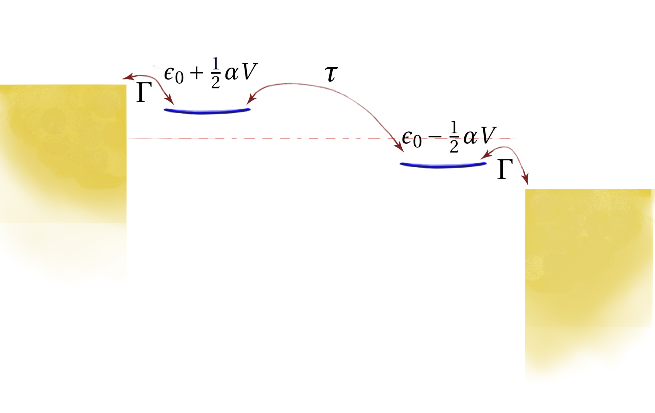
\includegraphics[height=.20\textheight]{pdf/non_interacting_schematics.pdf}\caption{non\hyp{}interacting}\label{fig:twositea}
    \end{subfigure}
    ~
    \begin{subfigure}[!tb]{0.48\textwidth}
        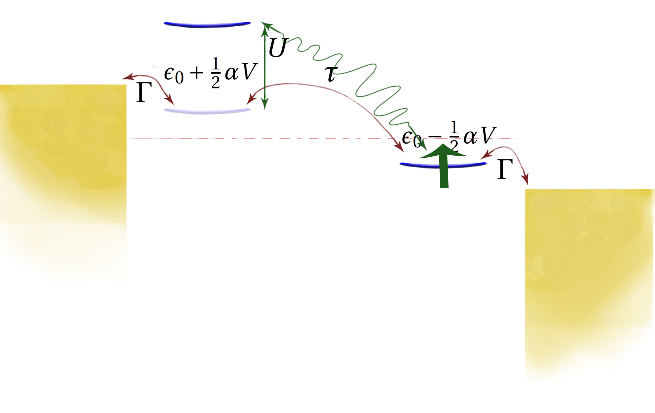
\includegraphics[height=.20\textheight]{pdf/interacting_schematics.pdf}\caption{Interacting}\label{fig:twositeb}
    \end{subfigure}
    \caption{Schematic pictures of the spinless two site model. The red dashed line denotes the Fermi-level. Figure~\ref{fig:twositea} shows the non\hyp{}interacting case, where $\Gamma$ is the molecule-lead coupling, $\epsilon \pm \frac{1}{2} \alpha V$ are the left (right) level and $\tau$ is the tunnelling strength between the levels. In Figure~\ref{fig:twositeb}, an electron (large green arrow) occupies the right level. The swirly line is meant to indicate an interaction with electrons on the left level, thereby raising the level with the capacitive interaction or charging energy $U$.} \label{fig:twosite}
\end{figure}

When no capacitive interaction is included (i.e. $U=0$), the common method (section~\ref{sec:synthesis}) can be applied to find the transmission analytically: \cite{perrinnano}\footnote{If the bias voltage is assumed to be distributed symmetrically over the leads, then the current can be found analytically as well. However, this serves no purpose in this discussion.}:
\begin{align*}
T(\epsilon) &= \frac{ (2\tau)^2 }{(\frac{\Gamma}{2})^2} \frac{(\frac{\Gamma}{2})^2}{(\epsilon-\epsilon_1)^2 + (\frac{\Gamma}{2})^2}\frac{(\frac{\Gamma}{2})^2}{(\epsilon-\epsilon_2)^2 + (\frac{\Gamma}{2})^2},
\end{align*}
where $\epsilon_{1,2} = \epsilon_0 \pm \frac{1}{2} \Delta$, where $\Delta$ is the level splitting in the presence of bias voltage given by $\Delta = \sqrt{ (\alpha V)^2+ 4\tau^2}$. 

For the two-site model including capacitive interactions, we assume that the chance a many-body state $\ket{\kappa}$ is occupied is proportional to the Boltzmann-factor $e^{ -\beta \braket{ \kappa\left| H \right| \kappa}} Z^{-1}$, where $Z$ is a normalisation constant and $H$ the full Hamiltonian including capacitive interactions.

It is illustrative for the application of the many-body Green's function (equation~\ref{eq:mbgfresult}) to consider the shapes of $G^{\lambda\pm}$. Their most important contribution in this context is simply the thermal average of the capacitive self-energy $\braket{\lambda\left|\Sigma^c\right|\lambda}$. The four $G^{\lambda\pm}$ are:
\begin{align*}
G^{\ket{00}\pm} &= \left[ \epsilon \begin{bmatrix} 1 & 0 \\ 0 & 1 \end{bmatrix} - \begin{bmatrix} \epsilon_0 + \frac{1}{2} \alpha V & -\tau \\
-\tau & \epsilon_0 - \frac{1}{2} \alpha V\end{bmatrix}  \pm \frac{\imath}{2} \begin{pmatrix} \Gamma & 0 \\ 0 & \Gamma \end{pmatrix} \right]^{-1}, \\
G^{\ket{10}\pm} &= \left[ \epsilon \begin{bmatrix} 1 & 0 \\ 0 & 1 \end{bmatrix} - \begin{bmatrix} \epsilon_0 + \frac{1}{2} \alpha V & -\tau \\
-\tau & \epsilon_0 - \frac{1}{2} \alpha V\end{bmatrix} - \begin{pmatrix} 0 & 0 \\ 0 & U \end{pmatrix} \pm \frac{\imath}{2} \begin{pmatrix} \Gamma & 0 \\ 0 & \Gamma \end{pmatrix} \right]^{-1}, \\
G^{\ket{01}\pm} &= \left[ \epsilon \begin{bmatrix} 1 & 0 \\ 0 & 1 \end{bmatrix} - \begin{bmatrix} \epsilon_0 + \frac{1}{2} \alpha V & -\tau \\
-\tau & \epsilon_0 - \frac{1}{2} \alpha V\end{bmatrix} - \begin{pmatrix} U & 0 \\ 0 & 0 \end{pmatrix} \pm \frac{\imath}{2} \begin{pmatrix} \Gamma & 0 \\ 0 & \Gamma \end{pmatrix} \right]^{-1},\\
G^{\ket{11}\pm} &= \left[ \epsilon \begin{bmatrix} 1 & 0 \\ 0 & 1 \end{bmatrix} - \begin{bmatrix} \epsilon_0 + \frac{1}{2} \alpha V & -\tau \\
-\tau & \epsilon_0 - \frac{1}{2} \alpha V\end{bmatrix} - \begin{pmatrix} U & 0 \\ 0 & U \end{pmatrix} \pm \frac{\imath}{2} \begin{pmatrix} \Gamma & 0 \\ 0 & \Gamma \end{pmatrix} \right]^{-1},
\end{align*}
where we see that adding an electron to e.g. $\ket{10}$ would add the energy $\epsilon_2$ and the capacitive interaction energy $U$. We see this quite clearly in the capacitive self-energy contribution of $G^{\ket{10}\pm}$. 

\subsection{Spinfull two site model}
When we include spin in the model, we are essentially keeping two copies of the model and add interaction. There is no spin-flip tunnelling. I use the ordered many-body basis $\left\{ \ket{\uparrow 1}, \ket{\downarrow 1}, \ket{\uparrow 2}, \ket{\downarrow 2}\right\}$. The Hamiltonian is:
\begin{align}
H_1 &= \begin{bmatrix} \epsilon_0 + \frac{1}{2} \alpha V & 0 & -\tau & 0 \\ 0 & \epsilon_0 + \frac{1}{2} \alpha V & 0 & -\tau\\ -\tau & 0 & \epsilon_0 - \frac{1}{2} \alpha V & 0 \\ 0 & -\tau & 0 & \epsilon_0 - \frac{1}{2} \alpha V\end{bmatrix},
\label{eq:spinfullhamiltonian}
\end{align} 
while the coupling matrices are:
\begin{align*}
\Gamma^L &= \begin{bmatrix} \Gamma & 0 & 0 & 0 \\ 0 & \Gamma & 0 & 0 \\ 0 & 0 & 0 & 0 \\  0 & 0 & 0 & 0\end{bmatrix},\\ \Gamma^R &= \begin{bmatrix} 0 & 0 & 0 & 0 \\ 0 & 0 & 0 & 0 \\ 0 & 0 & \Gamma & 0 \\ 0 & 0 & 0 & \Gamma \\ \end{bmatrix},
\end{align*}
and the capacitive self-energy is:
\begin{align*}
\Sigma^c &= \begin{bmatrix} \zeta U & 0 & 0 & 0\\ 0 & \zeta U & 0 & 0\\ 0 & 0 & 0 & 0\\ 0 & 0 & 0 & \xi U \end{bmatrix} n_{\uparrow 2} + \begin{bmatrix} \zeta U & 0 & 0 & 0\\ 0 & \zeta U & 0 & 0\\ 0 & 0 & \xi U & 0\\ 0 & 0 & 0 & 0 \end{bmatrix} n_{\downarrow 2} +\\
&\quad\begin{bmatrix} 0 & 0 & 0 & 0\\ 0 & \xi  U & 0 & 0\\ 0 & 0 & \zeta U & 0\\ 0 & 0 & 0 & \zeta U \end{bmatrix} n_{\uparrow 1} + \begin{bmatrix} \xi  U & 0 & 0 & 0\\ 0 & 0 & 0 & 0\\ 0 & 0 & \zeta U & 0\\ 0 & 0 & 0 & \zeta U \end{bmatrix} n_{\downarrow 1},
\end{align*}
where $\zeta U$ describes the strength of capacitive interaction between the left and right site (intersite), whereas $\xi U$ describes the strength of capacitive interaction on the left or right site (onsite).

The definitions for the coupling matrices $\Gamma^{R,L}$ allow us to directly calculate the transmission analytically in terms of the retarded and advanced Green's Function \emph{if only a single state is occupied}:
\begin{align*}
T(\epsilon) &= \Gamma^2 \left( G^+_{13} G^-_{31} + G^+_{14} G^-_{41} + G^+_{23} G^-_{32} + G^+_{24} G^-_{42} \right),
\end{align*}
where $\Gamma$ is the WBL coupling constant.Note that there is in principle a maximum of $4$ peaks. Because $\left(G^+\right)_{ij}^\star = G^-_{ji}$ in the energy-domain, there is no quantum interference and the function is real valued, as it should be. If the energy state is degenerate, the $G^\pm \rightarrow \mathscr{G}^\pm$ and quantum interference is possible.

\section{Expectations}
\label{sec:expectations}
Expectations for both flavors (spinless, spinfull) are discussed. 
\subsection{Spinless two-site model}
In section~\ref{sec:twositetransmission}, I will look at selected transmission figures for $U=0.0, 0.05, 0.15$ and $0.5$. The many-body character of the new theory makes it imperative to look at the many-body energies before I can make predictions about the different figures.

The initial guess for the self-consistency procedure (equation~\ref{eq:selfconsistency}) starts with the Boltzmann distribution as an initial guess, which specifies that only the lowest-energy many-body state is occupied. However, due to time constraints I have not used the self-consistency procedure, only working with the initial guess.

I conferred with Jose Celis Gil, and we agreed that the low temperature energy scale compared to the energy scales of the single-particle levels would cause rapid dissipation, implying a near\hyp{}equilibrium state, thereby justifying the approximation to the many-body occupation probabilities. Nevertheless, we did check this assumption. In Figure~\ref{fig:occprob}, we see that the self-consistent occupation probabilities (coloured diamonds) differ from the Boltzmann distribution (dashed lines) for $\left|V\right|\lesssim 0.10$. The theoretical mismatch of peak current in Ref.~\cite{perrinnano} has peaks at $\left|V\right|\approx 0.05$, so that the mismatch in occupation probabilities is only significant when no transmission peaks aligns with the Fermi-level. The mismatch is small when the levels start aligning, but seems sufficiently small that approximating by the Boltzmann distribution seems justifiable. In section~\ref{sec:resultsselfconsistencycalc}, I present a result that makes use of the self-consistency equation.

\begin{figure}[htb]
    \centering
    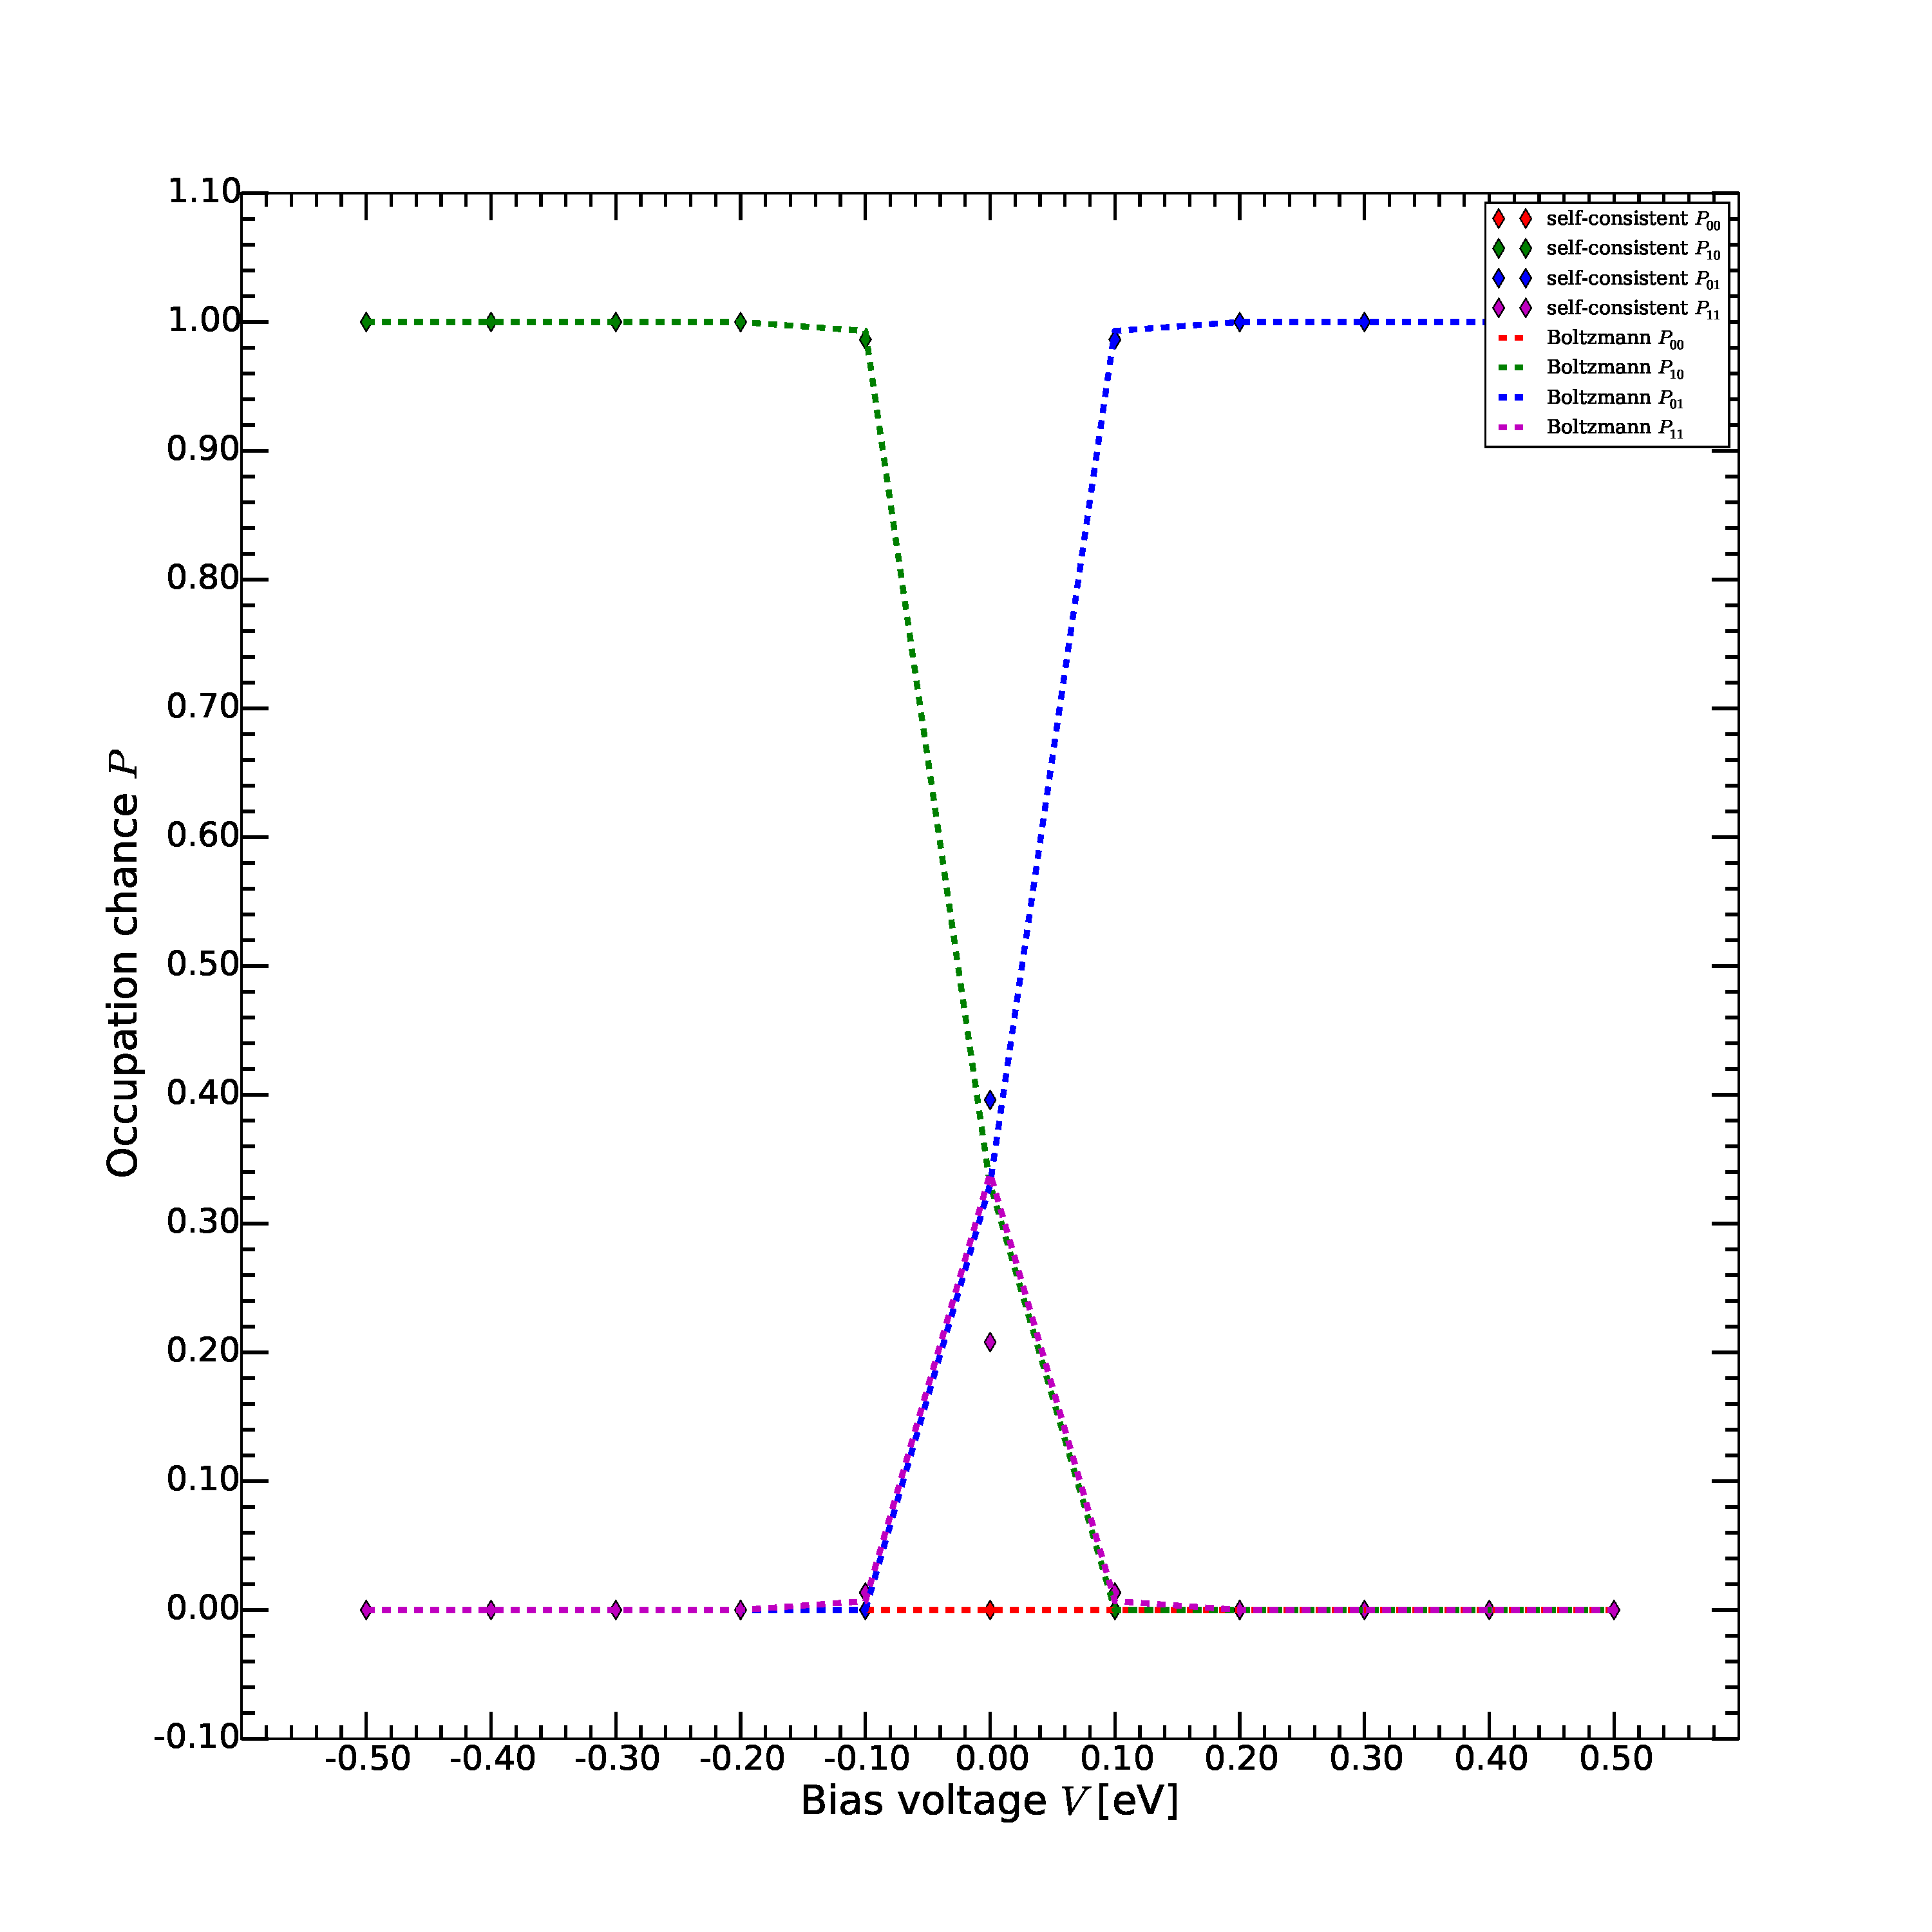
\includegraphics[width=.95\textwidth]{pdf/selfconsistent_low_temperature_1.pdf}
    \caption{Occupation probabilities $P_\kappa$ found by the self-consistency procedure (equation~\ref{eq:selfconsistency}) versus potential difference $V$ (coloured diamonds). The self-consistent results differ slightly from the Boltzmann distribution (dashed lines) around $V=0$, but do not differ from the Boltzmann distribution for $\left|V\right|\gtrsim 0.10$.}
    \label{fig:occprob}
\end{figure} \clearpage

Figure~\ref{fig:perrinenergy1} with $U=0.05$ is of interest because it shows the many-body character of my calculation, because the capacitive interaction enables the switch from $\ket{01}$ to $\ket{11}$ , which also causes a switch in transport behaviour. In the first state, there will be one transmission peak at $\epsilon_R$ and one at $\epsilon_L + U$. However, in the second state the second peak is also raised to $\epsilon_R+U$. Since this moves the levels further off-resonance, the transmission peak will be of lower height. 
\begin{figure}[htb]
    \centering
    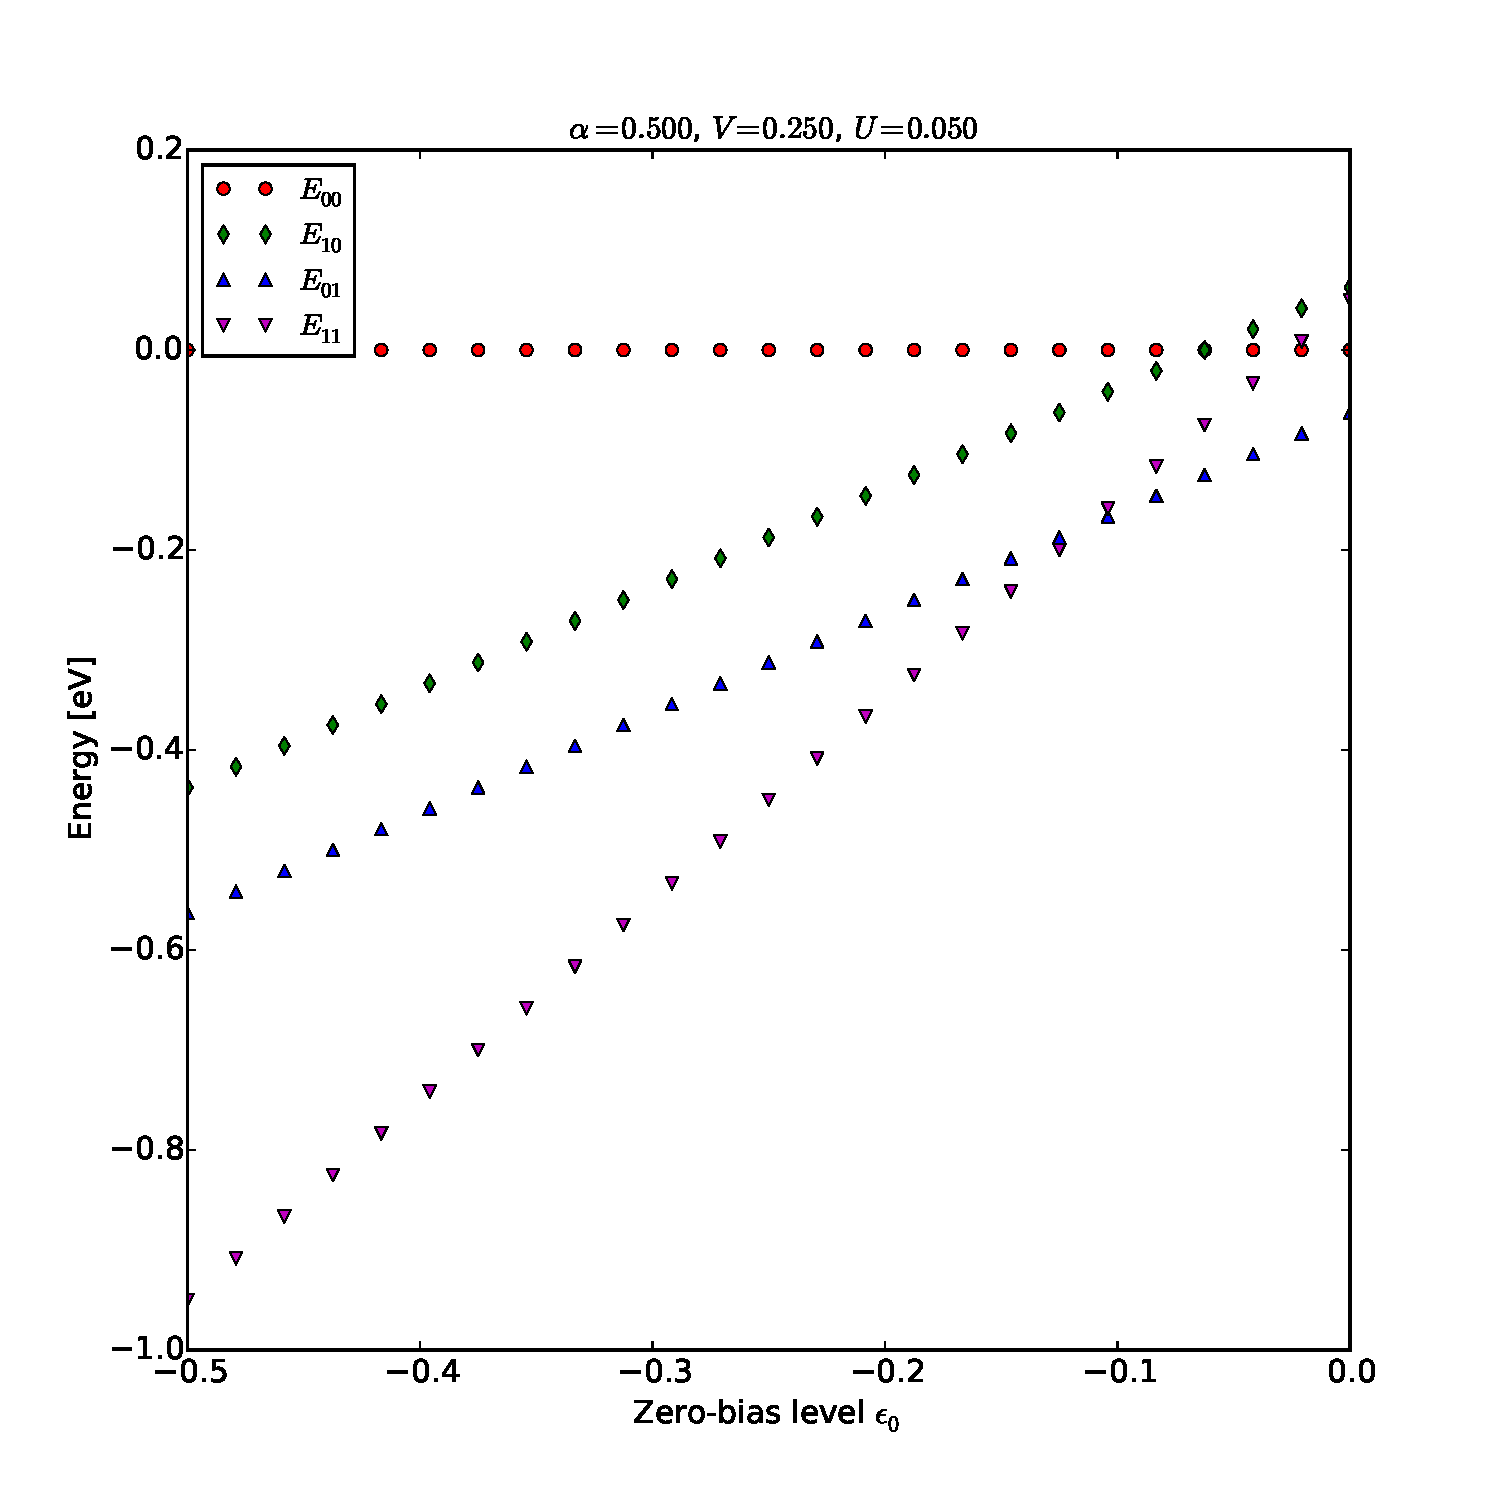
\includegraphics[height=.45\textheight]{pdf/energy/perrin_distribution_u1.pdf}
    \caption{Energy of many-body states versus zero-bias level $\epsilon_0$ for the spinless two-site model at $U=0.05$. The subscripts $E_{ij}$ refer to the many-body state $\ket{i j}$. At $\epsilon_0 \approx 0$, there is one electron on the right level. Lowering $\epsilon_0$ past ~$-0.12$ indicates a shift to an occupation of both the left and right levels.  }
    \label{fig:perrinenergy1}
\end{figure} 

 
\subsection{Spinfull two-site model} 
In this section, I present the energies of the spinfull model for $U=0.05$, $\zeta=1.00$, $\xi=1.00$, parameters that to match the transmission figure presented in section~\ref{sec:twositetransmission}.
 
\begin{figure}[htb]
    \centering
    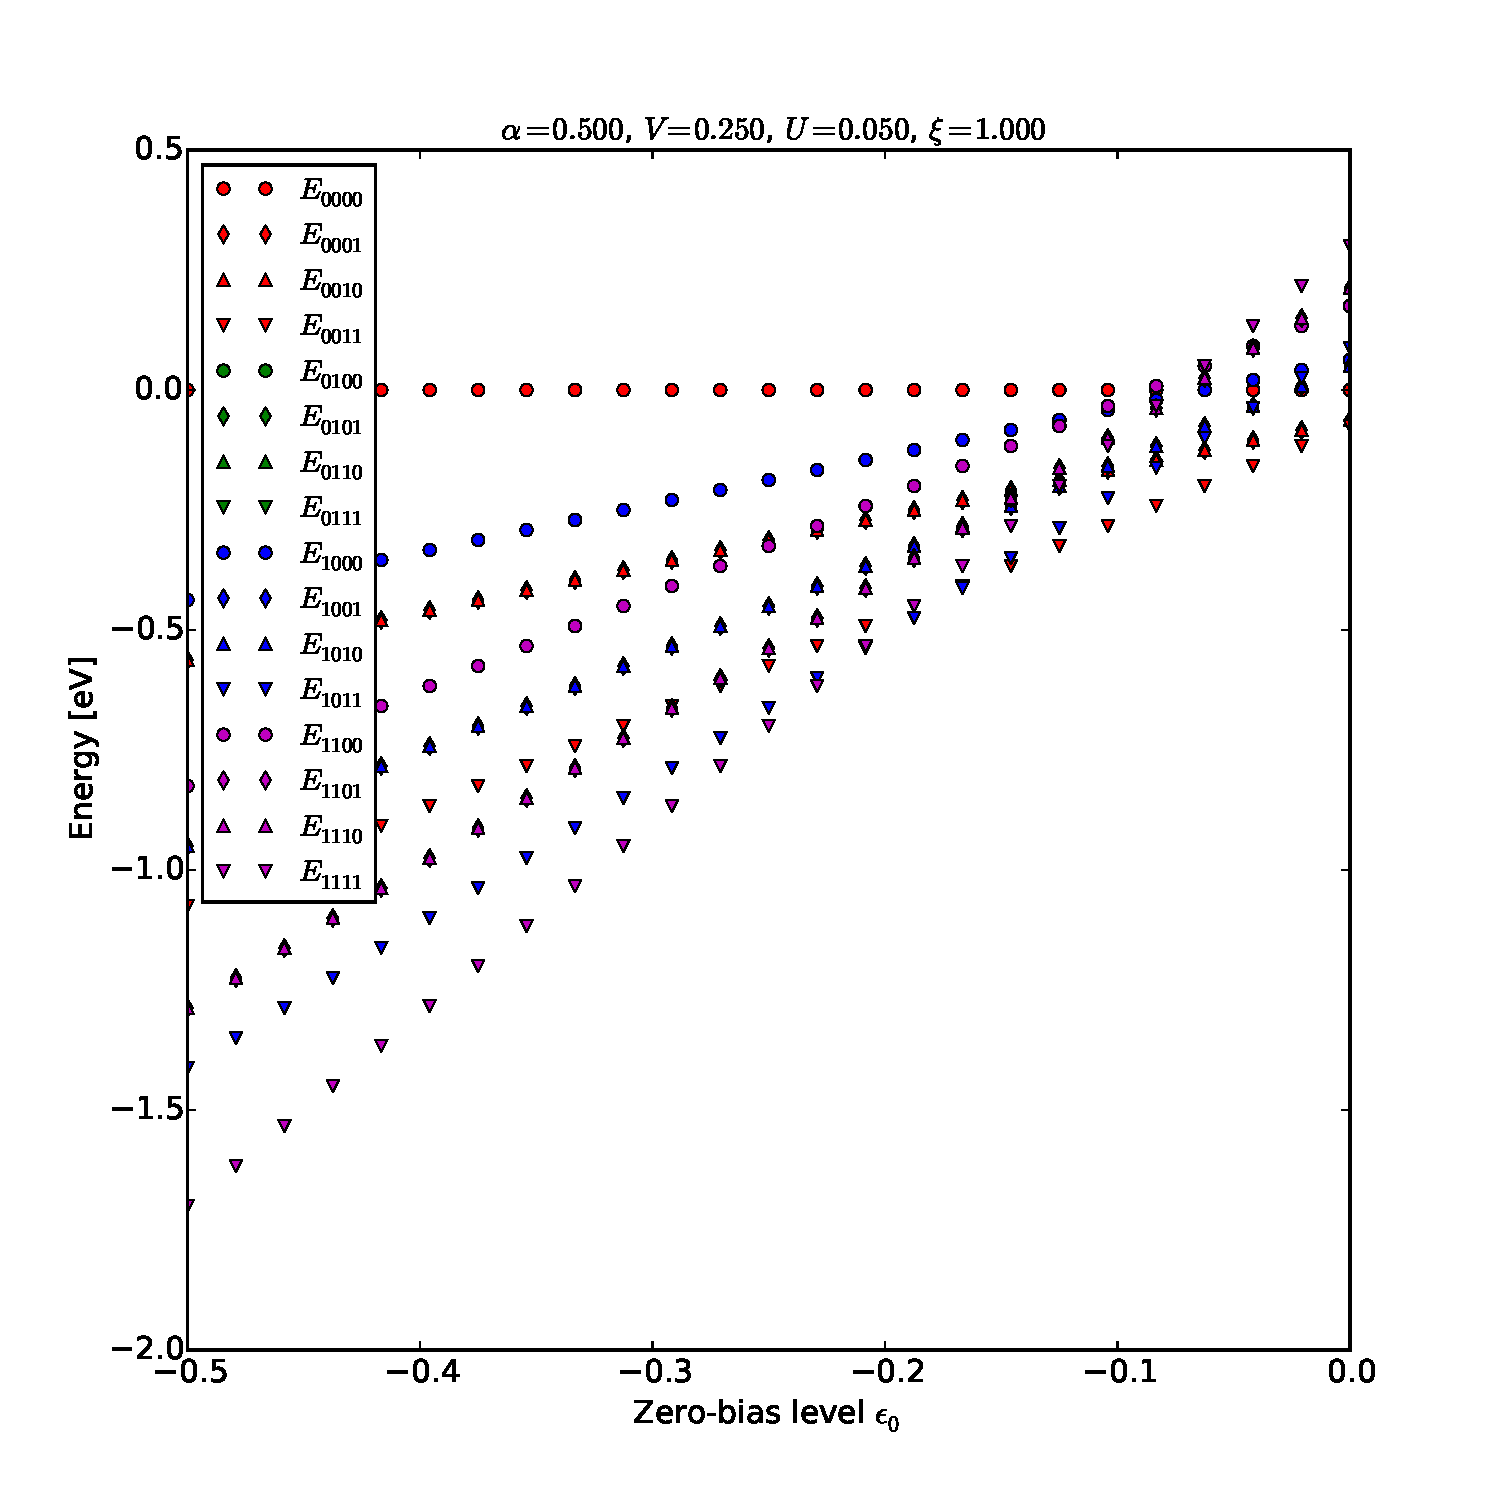
\includegraphics[height=.45\textheight]{pdf/energy/pespin_distribution_u1_k2.pdf}
    \caption{Energy of many-body states versus zero-bias level $\epsilon_0$ for the spinfull two-site model. In this figure, $U=0.05$, $\zeta=1.00$, $\xi=1.00$. The lowest energy state is $\ket{0011}$ for $\epsilon_0\gtrsim -0.15$, which then switches to $\ket{1011}$ before switching to $\ket{1111}$ at $\epsilon_0 \lesssim -0.20$.}
    \label{fig:perspinenergy12}
\end{figure}  


The Fock-space of occupation states for the spinfull model has dimension $2^4$, so that there are that many energies in the figures. In Figure~\ref{fig:perspinenergy12} I see similar behaviour as in the spinless case. There are switches between different many-body states, which are expected to cause some transmission peaks to shift by $\zeta U$ or $\xi U$ or both. The specifics of the many-body states are indicated in their captions.
\section{Transmission}
\label{sec:twositetransmission}
Transmissions for both flavors (spinless, spinfull) are discussed. 
\subsection{Spinless two-site model}
First, I want to look at the transmission for the spinless model.Figure~\ref{fig:spinlesstransmission} compares an interacting ($U=0.5$) transmission spectrum versus a non-interacting one. The effect of interaction is apparently to suppress the transmission peak height and move the rightmost peak outwards by $U$. 
\begin{figure}[htb]
    \centering
    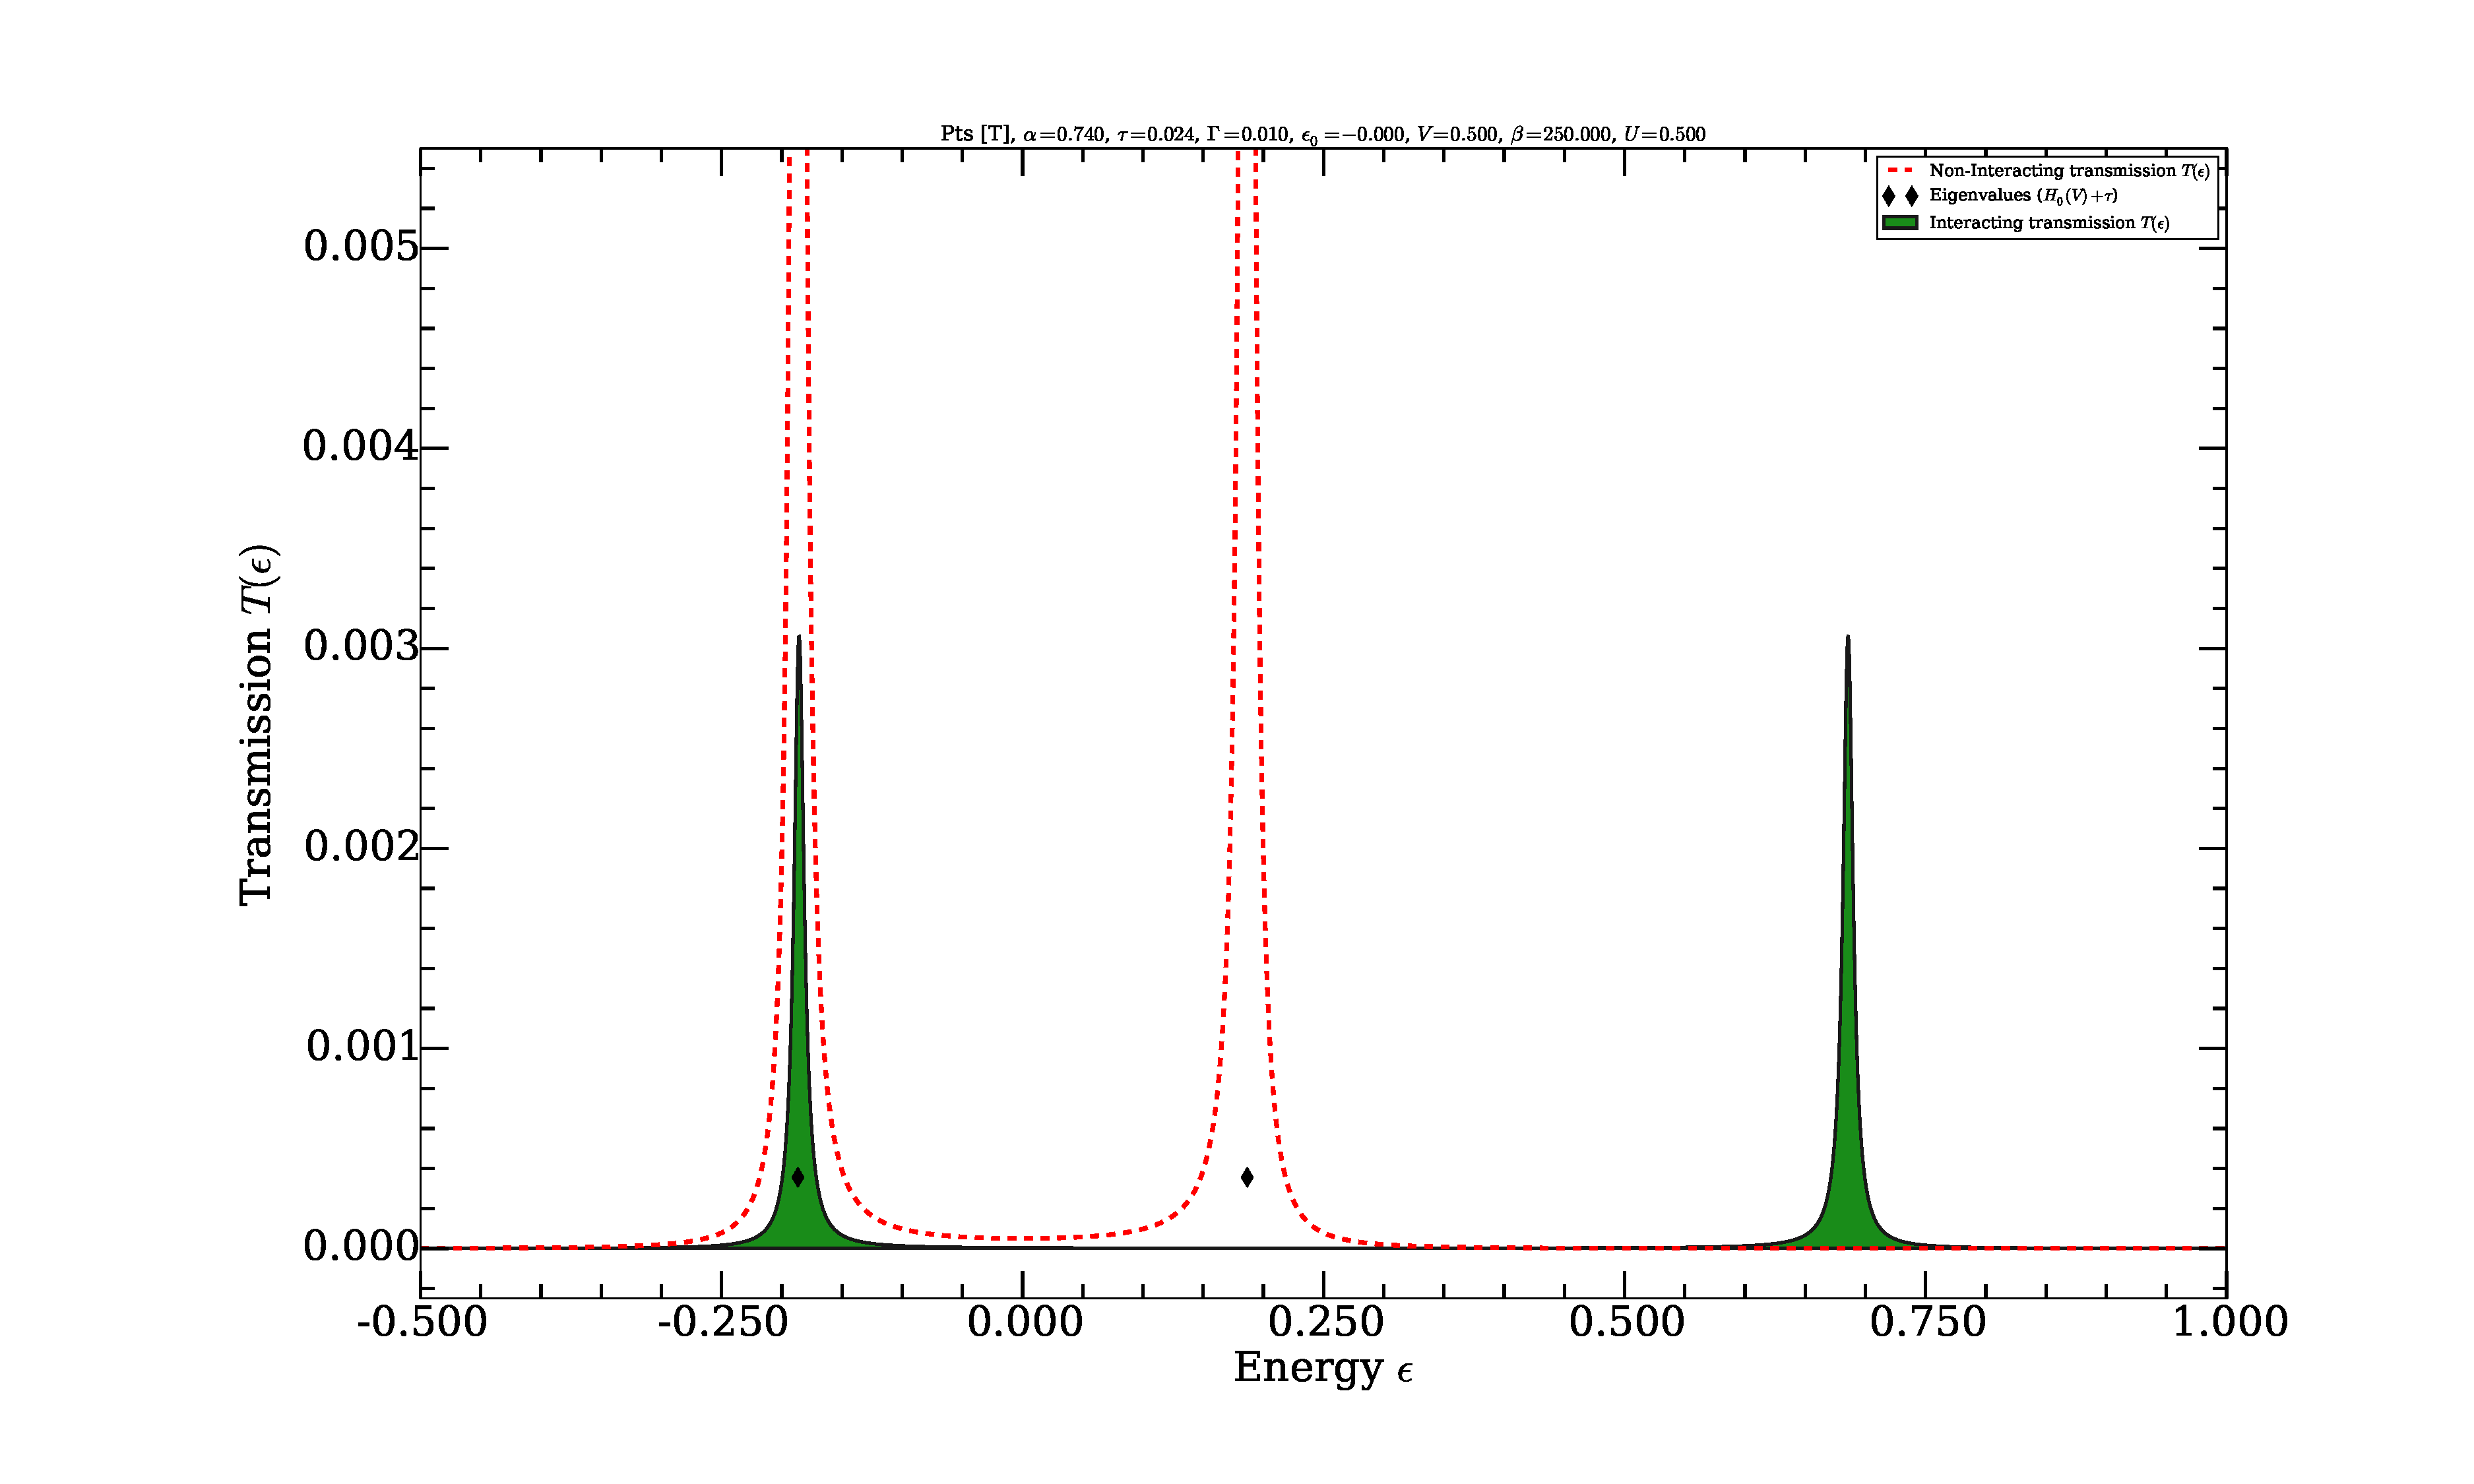
\includegraphics[height=.35\textheight,clip=true,trim=5cm 2cm 4cm 3cm]{pdf/trans/perrin_two_site.pdf}
    \caption{Non-interacting (dashed red) and interacting (green) transmission spectra for $\alpha=0.74$, $\tau=0.024$, $\Gamma=0.010$, $\epsilon_0 = 0$, $V=0.50$ and $U=0.5$. In comparison with the non-interacting transmission, the peaks have dropped significantly and the rightmost peak is exactly $U$ removed from the corresponding eigenvalue (black diamonds).}
    \label{fig:spinlesstransmission}
\end{figure}

The interacting transmission spectrum looks similar to a non-interacting transmission spectrum, but the peak values differ. It is perhaps illustrative to consider Figure~\ref{fig:perrin_effective}. In this figure the `effective parameters' change almost linearly with increasing $U$. The effective parameters are those parameters for which the features of the transmission agree with a non-interacting model ignoring peak height.
\begin{figure}[htb]
    \centering
    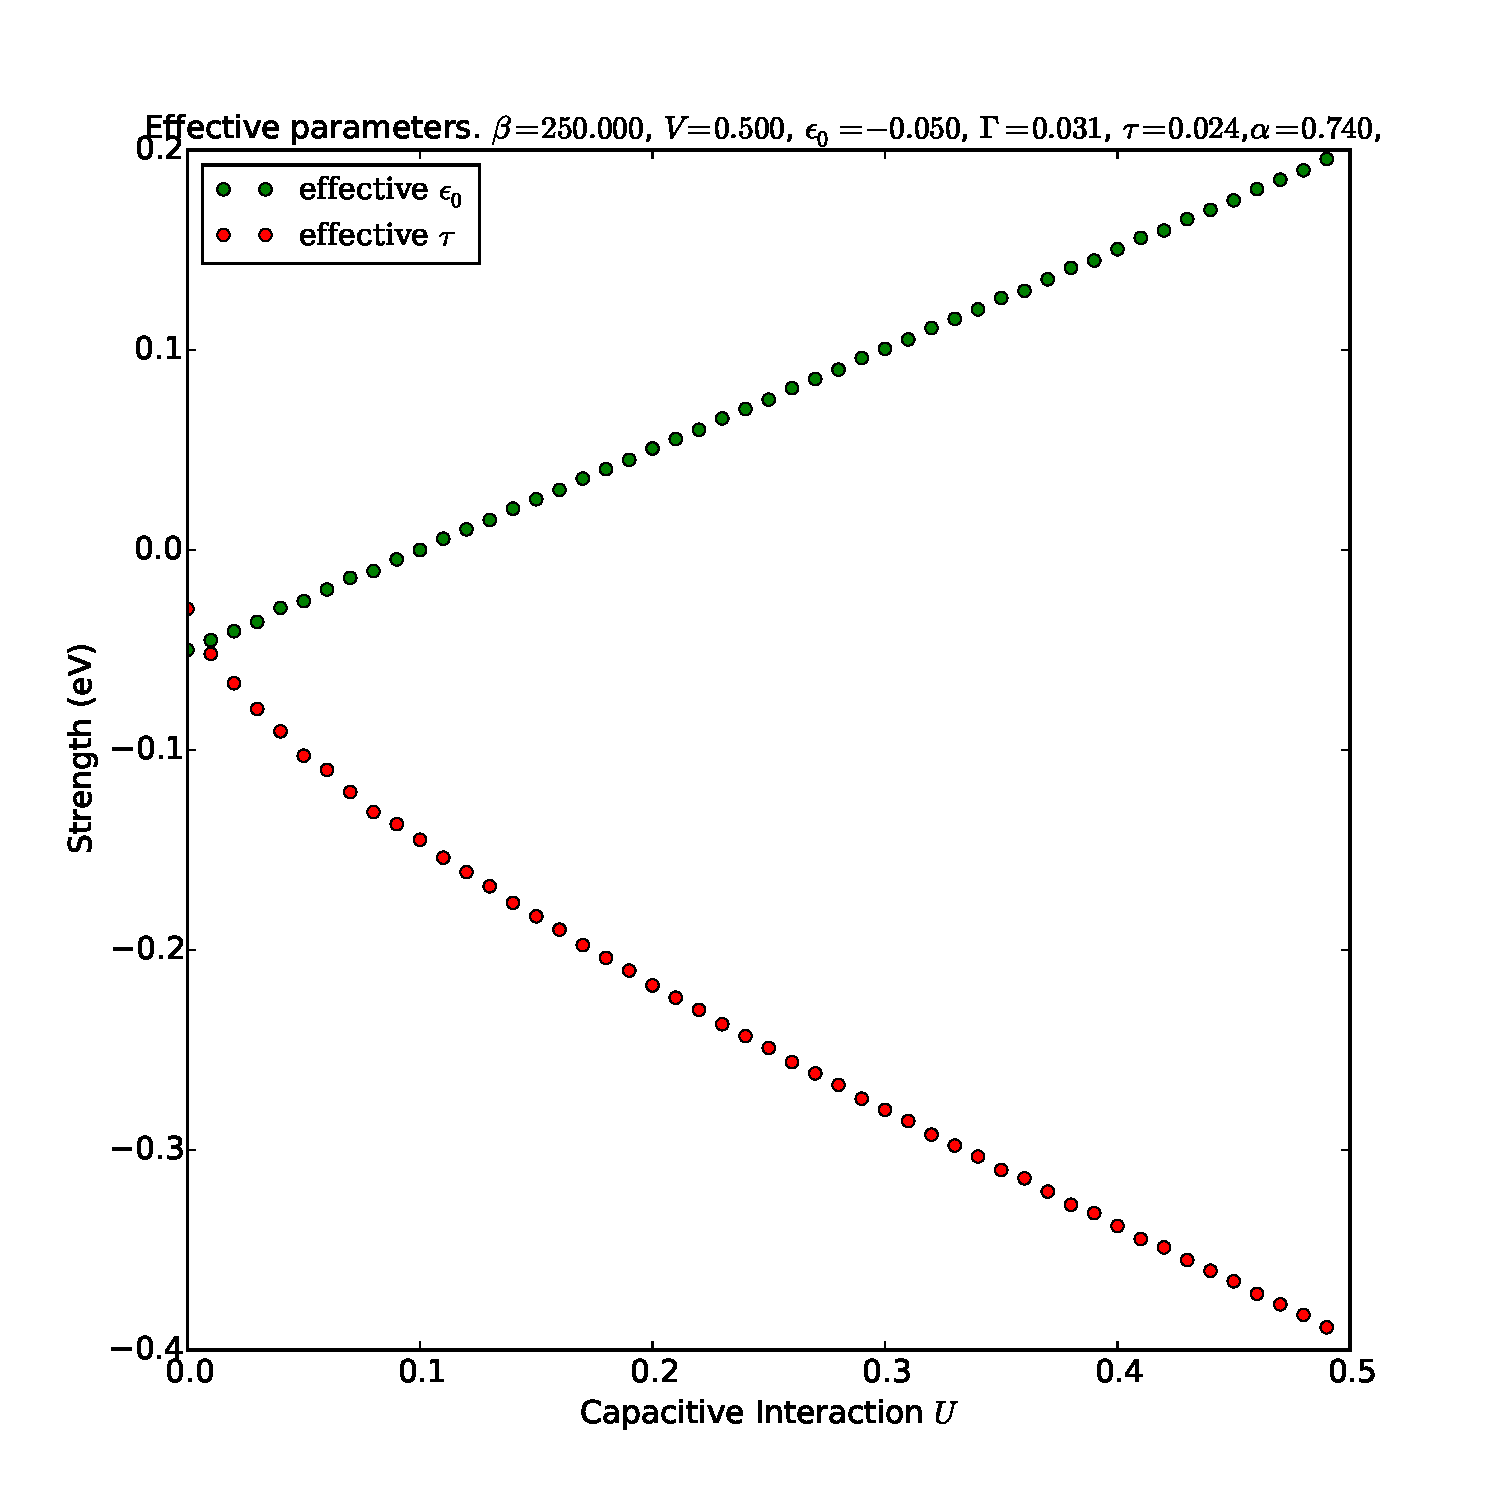
\includegraphics[height=.35\textheight]{pdf/trans/perrin_effective.pdf}
    \caption{In this figure, $\epsilon_0$ and $\tau$ are for a non-interacting model that is fitted to an interacting model, leading to `effective' parameters. This ignores the fact that the peaks of an interacting are suppressed. }
    \label{fig:perrin_effective}
\end{figure}


These figures indicate that a mismatch in peak values such as that found in Ref.~\cite{perrinnano} may well be explained in terms of capacitive interaction. Here, the shape would be fitting for a two-site model without capacitive interaction, but the amplitude element of capacitive interaction is merely seen as quantitative disagreement. This notion will be discussed further in section~\ref{sec:perrin}. 

\subsection{Spinfull two-site model}
I now want to look at the transmission of the spinfull model \emph{in comparison} with that of the spinless model. First, recall that $\zeta$ describes the intersite interaction while $\xi$ the onsite interaction. Given the large amount of possible pictures, here I present only those that are interesting results that are distinct from the spinless model with the exception of Figure~\ref{fig:transmap34} which has extremely strong onsite interaction $\xi$ such that the two models are expected to converge. 
  
\begin{figure}[htb]
    \centering
    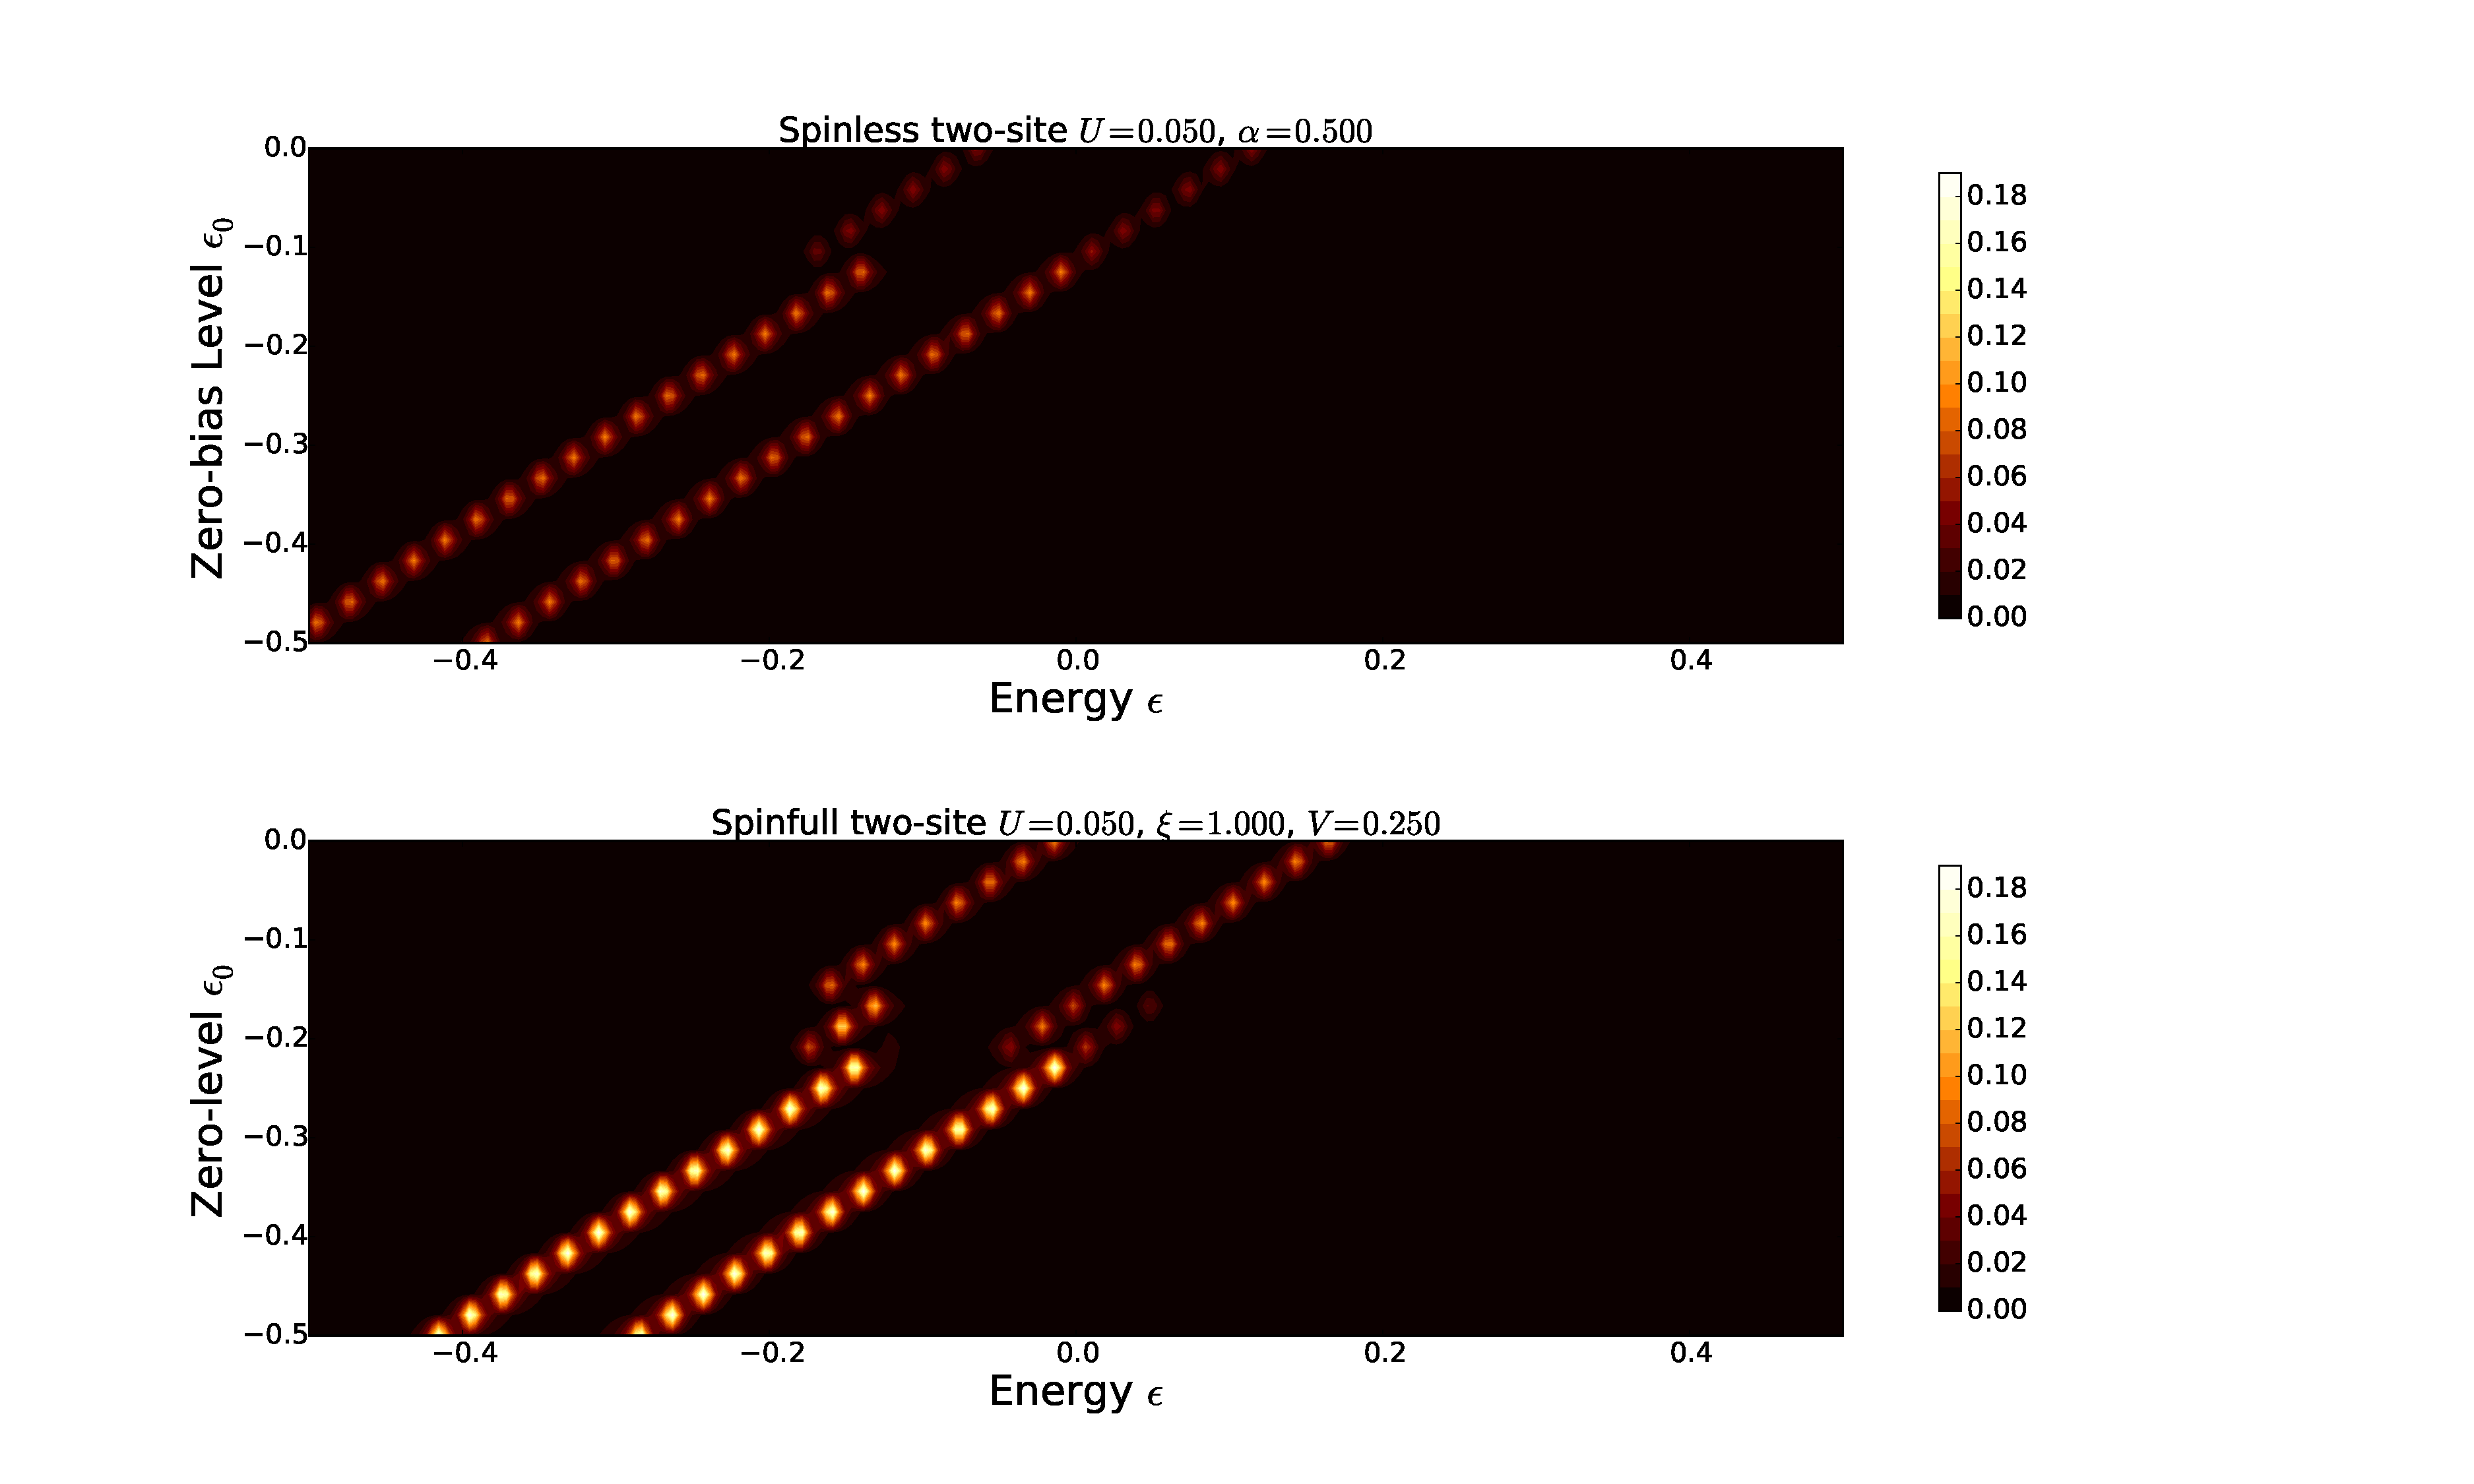
\includegraphics[height=.38\textheight]{pdf/map/transmap_u1_k2.pdf}
    \caption{In this figure, $U=0.05, \zeta=1.00, \xi=1.00$. A distinct difference is very clear, with a three-peak transmission spectrum making a short appearance. See the main text for explanation.}
    \label{fig:transmap12}
\end{figure} 
\begin{figure}[htb]
    \centering
    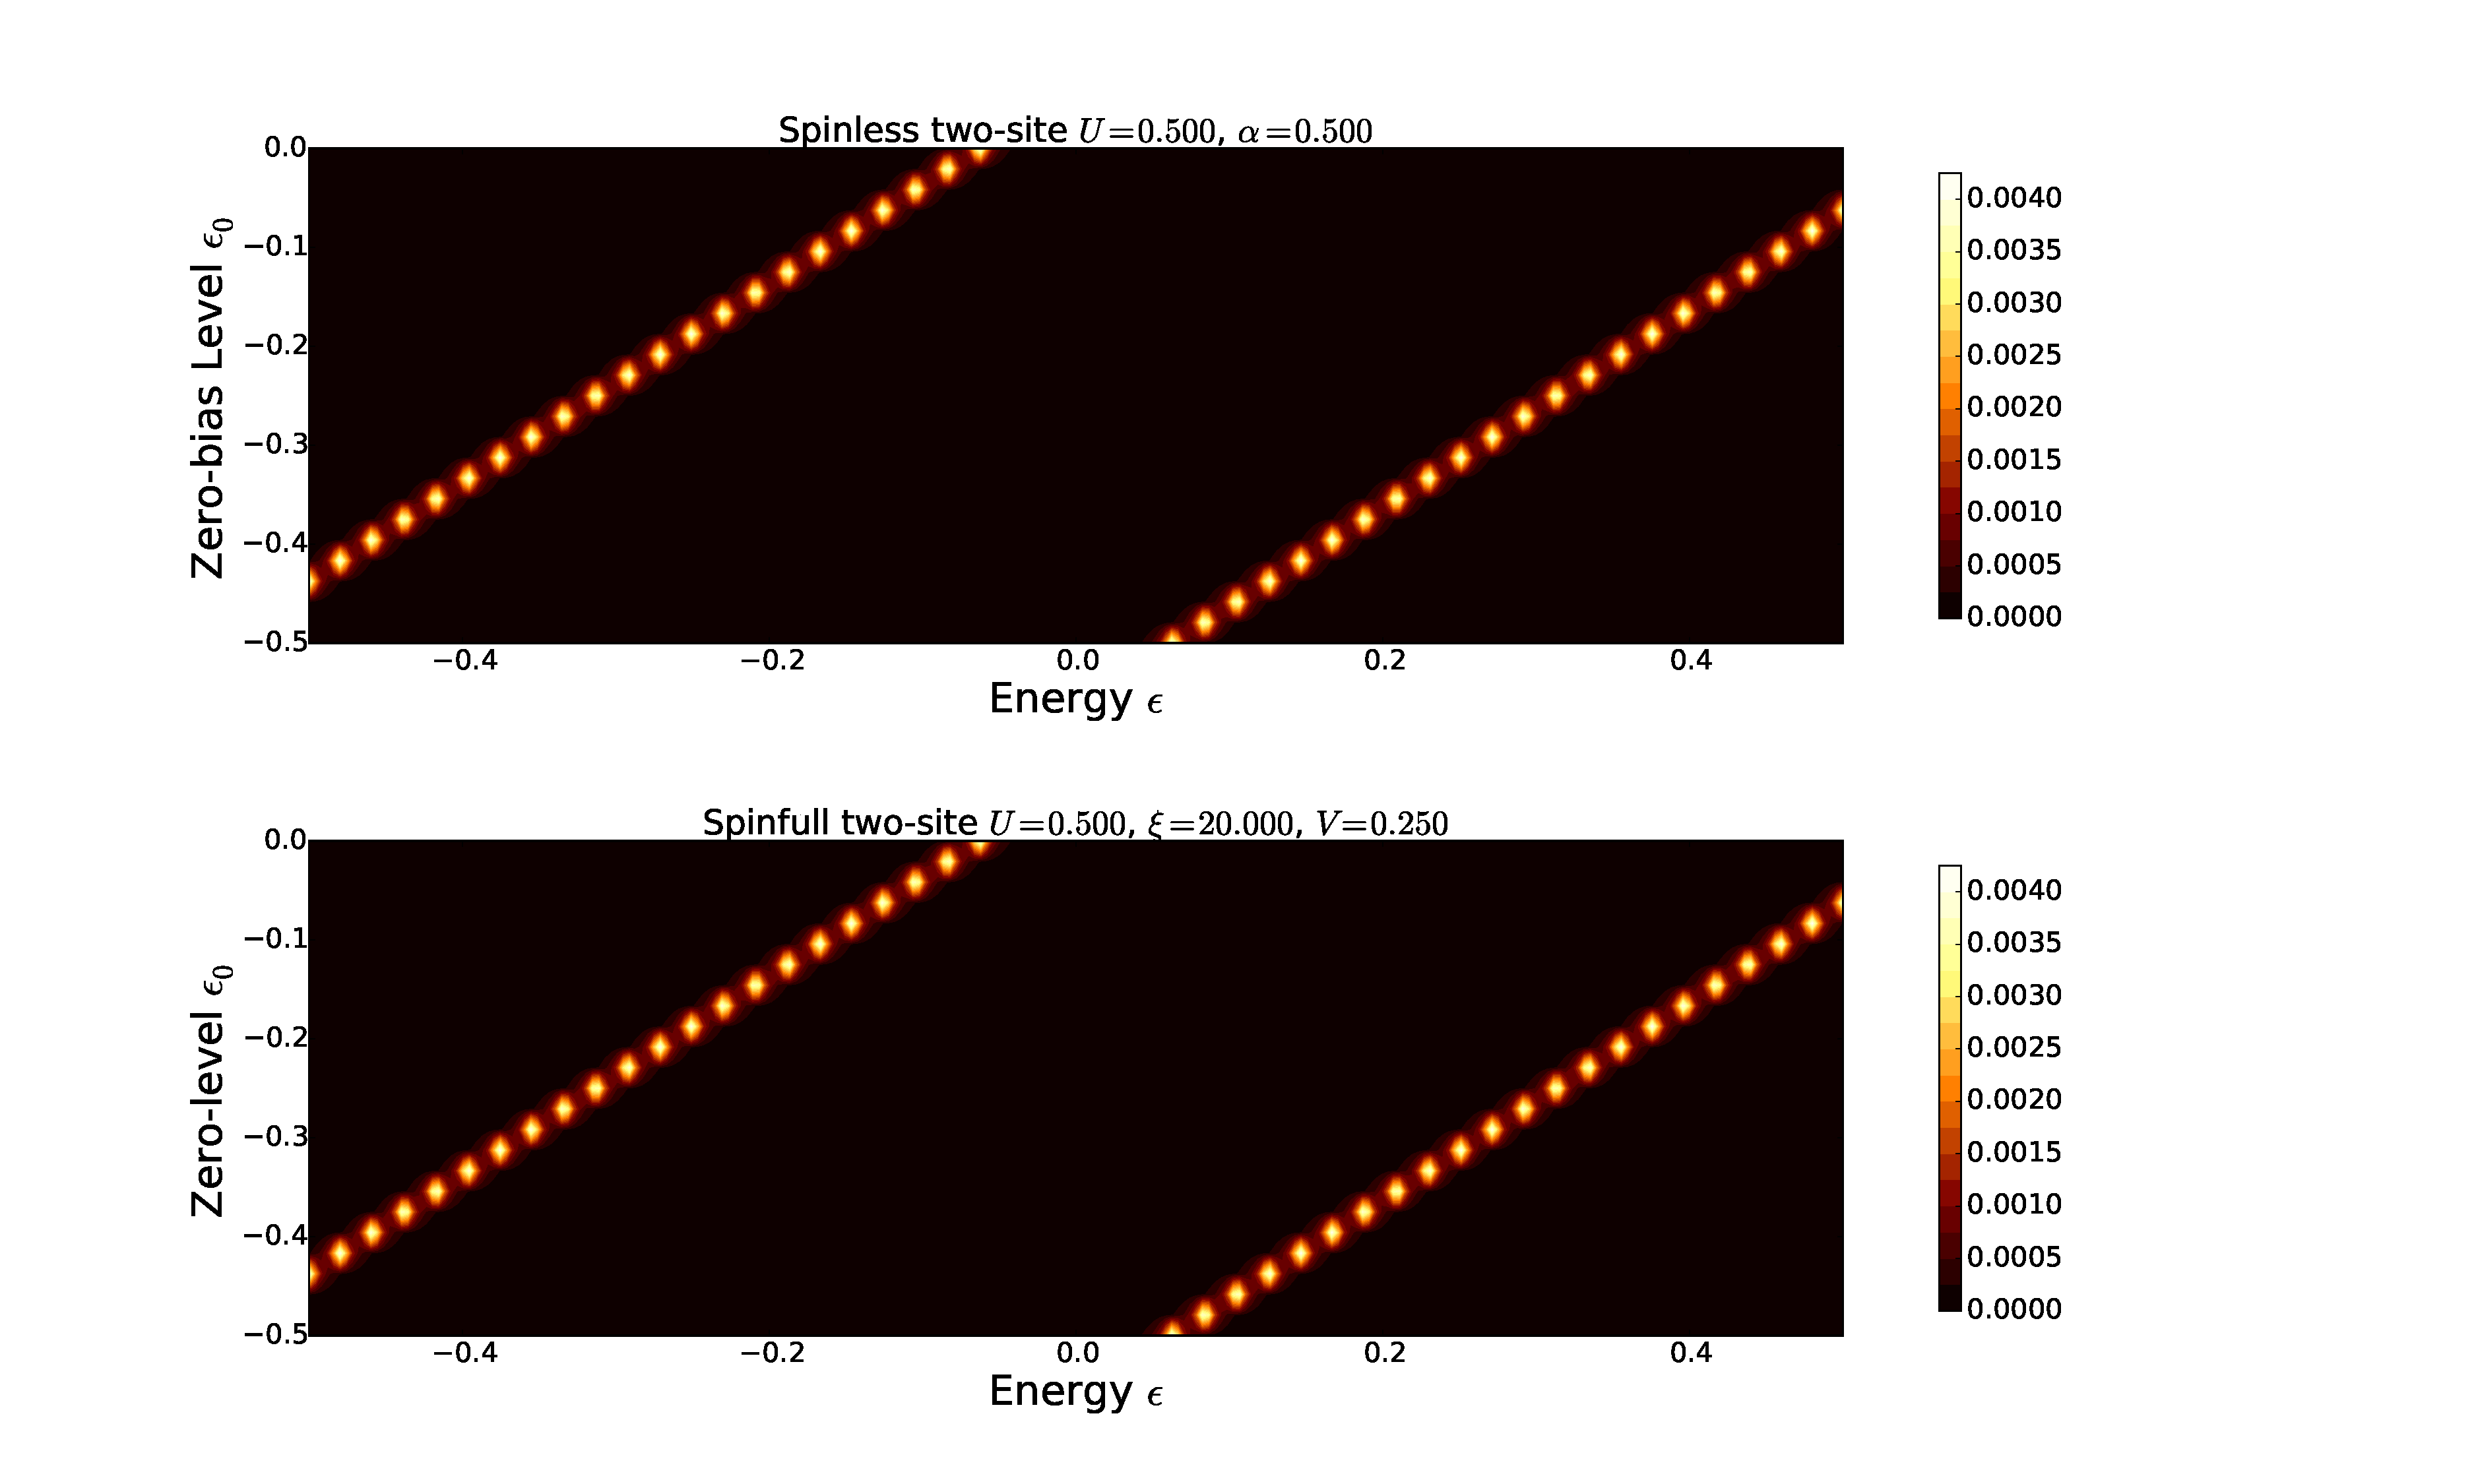
\includegraphics[height=.38\textheight]{pdf/map/transmap_u3_k4.pdf}
    \caption{In this figure, $U=0.15, \zeta=1.00, \xi=20.00$. The two models converge, which is expected for this $\xi$. See the main text for explanation.}
    \label{fig:transmap34}
\end{figure}

Evidence of the many-body character of both models is clear in Figure~\ref{fig:transmap12}, where there is one switch in transmission peaks for the spinless model and two switches for the spinfull model. The spinless model switches from $\ket{01}$ to $\ket{11}$ (Figure~\ref{fig:perrinenergy1}), displacing one peak by an amount $U$ which agrees well with the transmission figure.  The spinfull model, on the other hand, switches from $\ket{0011}$ to either $\ket{0111}$ or $\ket{1011}$ before switching to $\ket{1111}$ (Figure~\ref{fig:perspinenergy12}). Note that the rightmost peaks corresponds to the left site, and the leftmost peak corresponds to the right site. The first switch displaces the leftmost peak\footnote{Adding an electron to the left level adds $U$ to the right level, which displaces the left peak.}and seems to have placed a third peak at the rightmost peak plus $U$, a likely result because the energy states are degenerate. The second switch then displaces the leftmost peak by $\xi U$. 
 
Figure~\ref{fig:transmap34} is that figure for which the onsite energy $\xi U$ dominates so that only a single copy of the spinless model is active at any time. Therefore, not only do the peaks in transmission happen at the same location, but they are also of the same height.
\section{Current parameter sweeps}
\label{sec:twositeparamsweep}
The most interesting parameter sweeps are those that affect the many-body states. The current through a single-molecule has a well known feature called the Coulomb Diamond \cite{seldenthuis, perrin} in a plot of the gate voltage versus the bias voltage and coloured by the current. The gate voltage corresponds approximately to the zero-bias level, $V_\text{gate} \approx \epsilon_0$. Each diamond corresponds to a different charge state. As I only present current parameter sweeps for the spinless case, for which throughout $-0.5 < \epsilon_0 < 0$ there are two occupied many-body states, we expect one diamond to form.  

\begin{figure}[htb]
    \centering
    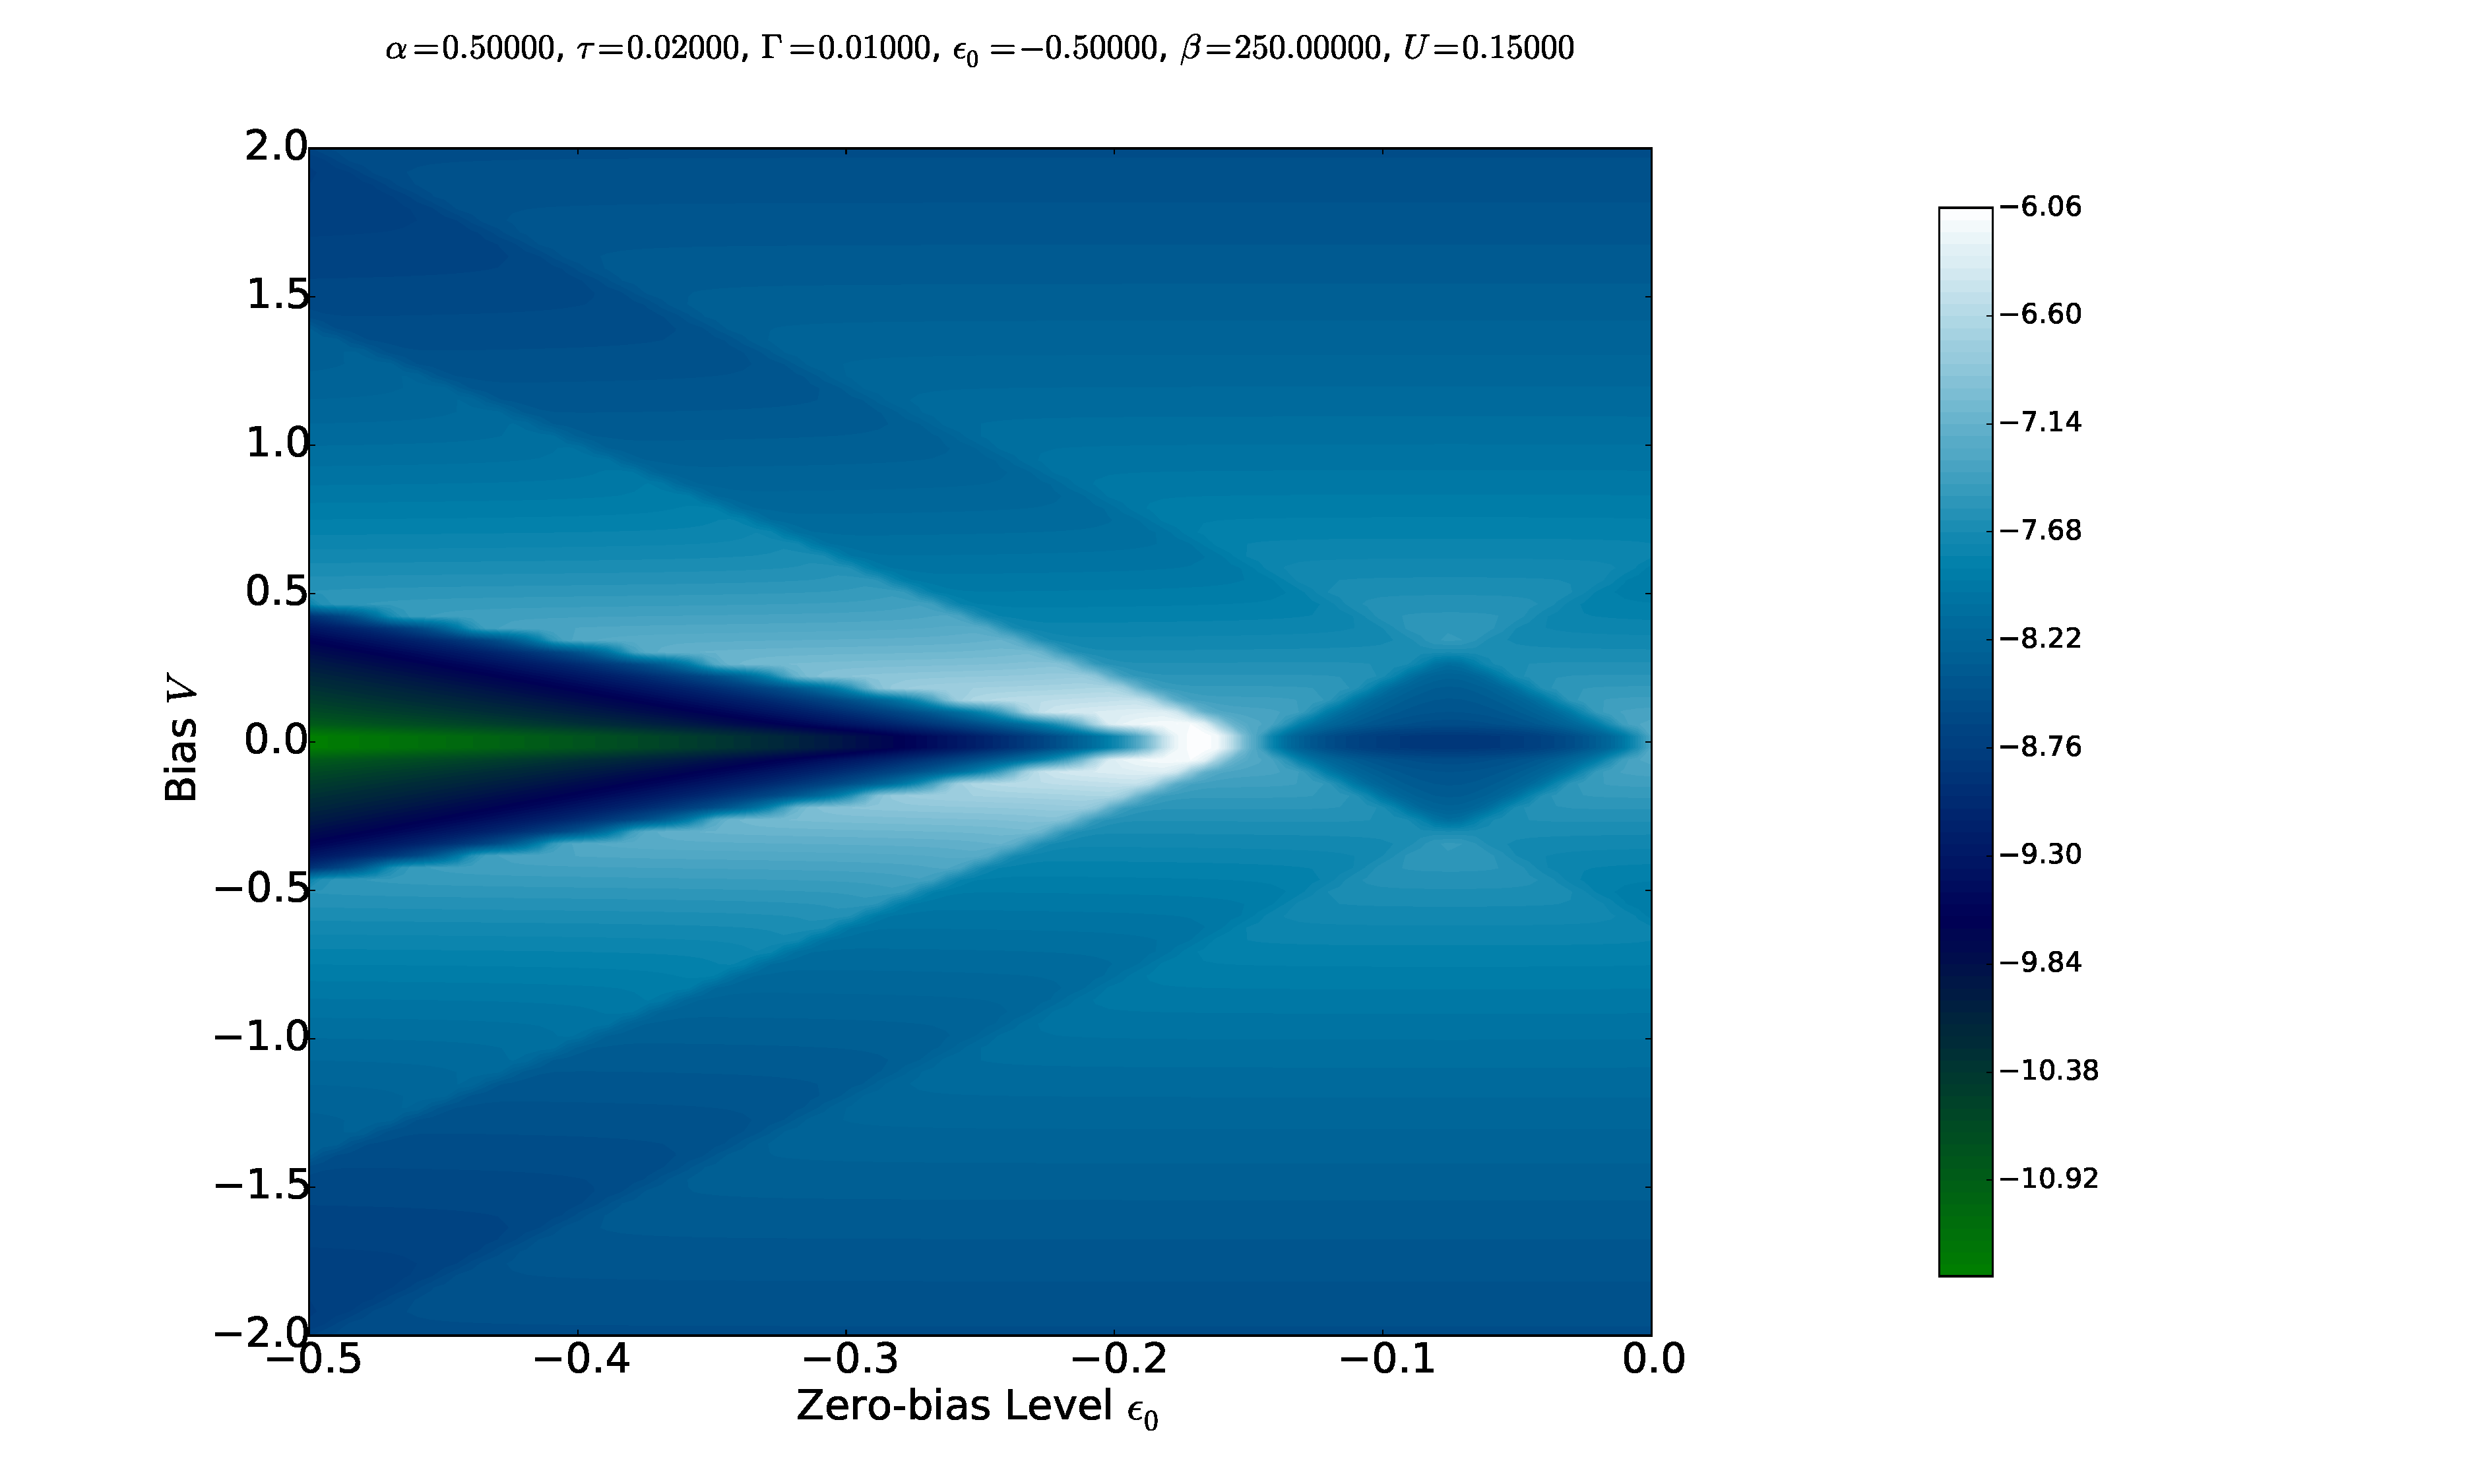
\includegraphics[height=.38\textheight]{pdf/coulombd/current_map_u2.pdf}
    \caption{In this figure, $U=0.15$. The Coulomb diamond is singificantly clearer and again has width $U$. The triangular area to the left of the diamond corresponds to the next charge state. The distinct lines correspond to the bias window increasing to encompass a second transmission peak.The colours are based on the $^{10}\text{log}\left|I(V)\right|$, so that the NDC is implied because $I(V) = -I(-V)$.}
    \label{fig:currentmap2}
\end{figure} 

Figures~\ref{fig:currentmap2} and ~\ref{fig:diamond50} show the onset of the Coulomb diamond and that its width exactly equals the capacitive interaction strength $U$. The left triangular area visible in most of the figures is the next charge state, which for the spinless model is the state $\ket{11}$ whereas the Coulomb diamond is associated with $\ket{01}$ (at positive bias). 

I explored the characteristics of the Coulomb Diamond a bit more. Analytically, the corresponding charge state leads to the following Green's function (section~\ref{sec:twosite}):
\begin{align*}
G^{\ket{01}\pm} &= \left[ \epsilon \begin{bmatrix} 1 & 0 \\ 0 & 1 \end{bmatrix} - \begin{bmatrix} \epsilon_0 + \frac{1}{2} \alpha V & -\tau \\
-\tau & \epsilon_0 - \frac{1}{2} \alpha V\end{bmatrix} - \begin{pmatrix} U & 0 \\ 0 & 0 \end{pmatrix} \pm \frac{\imath}{2} \begin{pmatrix} \Gamma & 0 \\ 0 & \Gamma \end{pmatrix} \right]^{-1},
\end{align*}
so that the transmission peaks should be found at eigenvalues of $\begin{bmatrix} \epsilon_0 + \frac{1}{2} \alpha V+U & -\tau \\
-\tau & \epsilon_0 - \frac{1}{2} \alpha V\end{bmatrix}$.

Section~\ref{sec:twositetransmission} showed that the transmission peak locations change linearly with $\epsilon_0$, at least within a single charge state. Consider a state which starts on resonance, i.e. a transmission peak is within the bias window immediately. In this scenario, the leftmost transmission peak is within the bias window. Upon lowering $\epsilon_0$, the two transmission peaks shift slightly to the left. At higher bias, the intersection of the leftmost peak with the bias window is still at a lower bias voltage than that of the rightmost peak, but at a larger bias voltage than at higher $\epsilon_0$. As the lowering continues, the two values slowly approach each other. This is the corner of the Coulomb diamond.

Next, the the rightmost peak has the lower bias voltage at which it intersects the bias window and this intersection value is shrinking. This continues until the point where the rightmost peak is completely inside the bias window. This closes the diamond. 

The expectation is that the next charge state is then available, and indeed I find that the energies dictate the molecule now occupies the next charge state.

The rate at which the transmission lines move outward depends almost entirely on $\alpha$. While it is technically the level-splitting $\Delta$, it is trivial that as the only growing term it will soon dominate that term, leading to $\Delta \approx \alpha V$. As such, I expect that the height of the Coulomb diamond depends mostly on $\alpha$. 

Indeed, this is what we find Figures~\ref{fig:diamond50} and ~\ref{fig:diamond75}. These figures also show the co-tunneling current within the diamond clearly. Here, the symmetry dictates that $I(V)=-I(-V)$, so that the co-tunneling current has a sign switch around $V=0$. Furthermore, the Stark effect pulls the sites further from each other, which leads to a reduction of the co-tunnelling current that is just barely visible. 
\begin{figure}[htb]
    \centering
    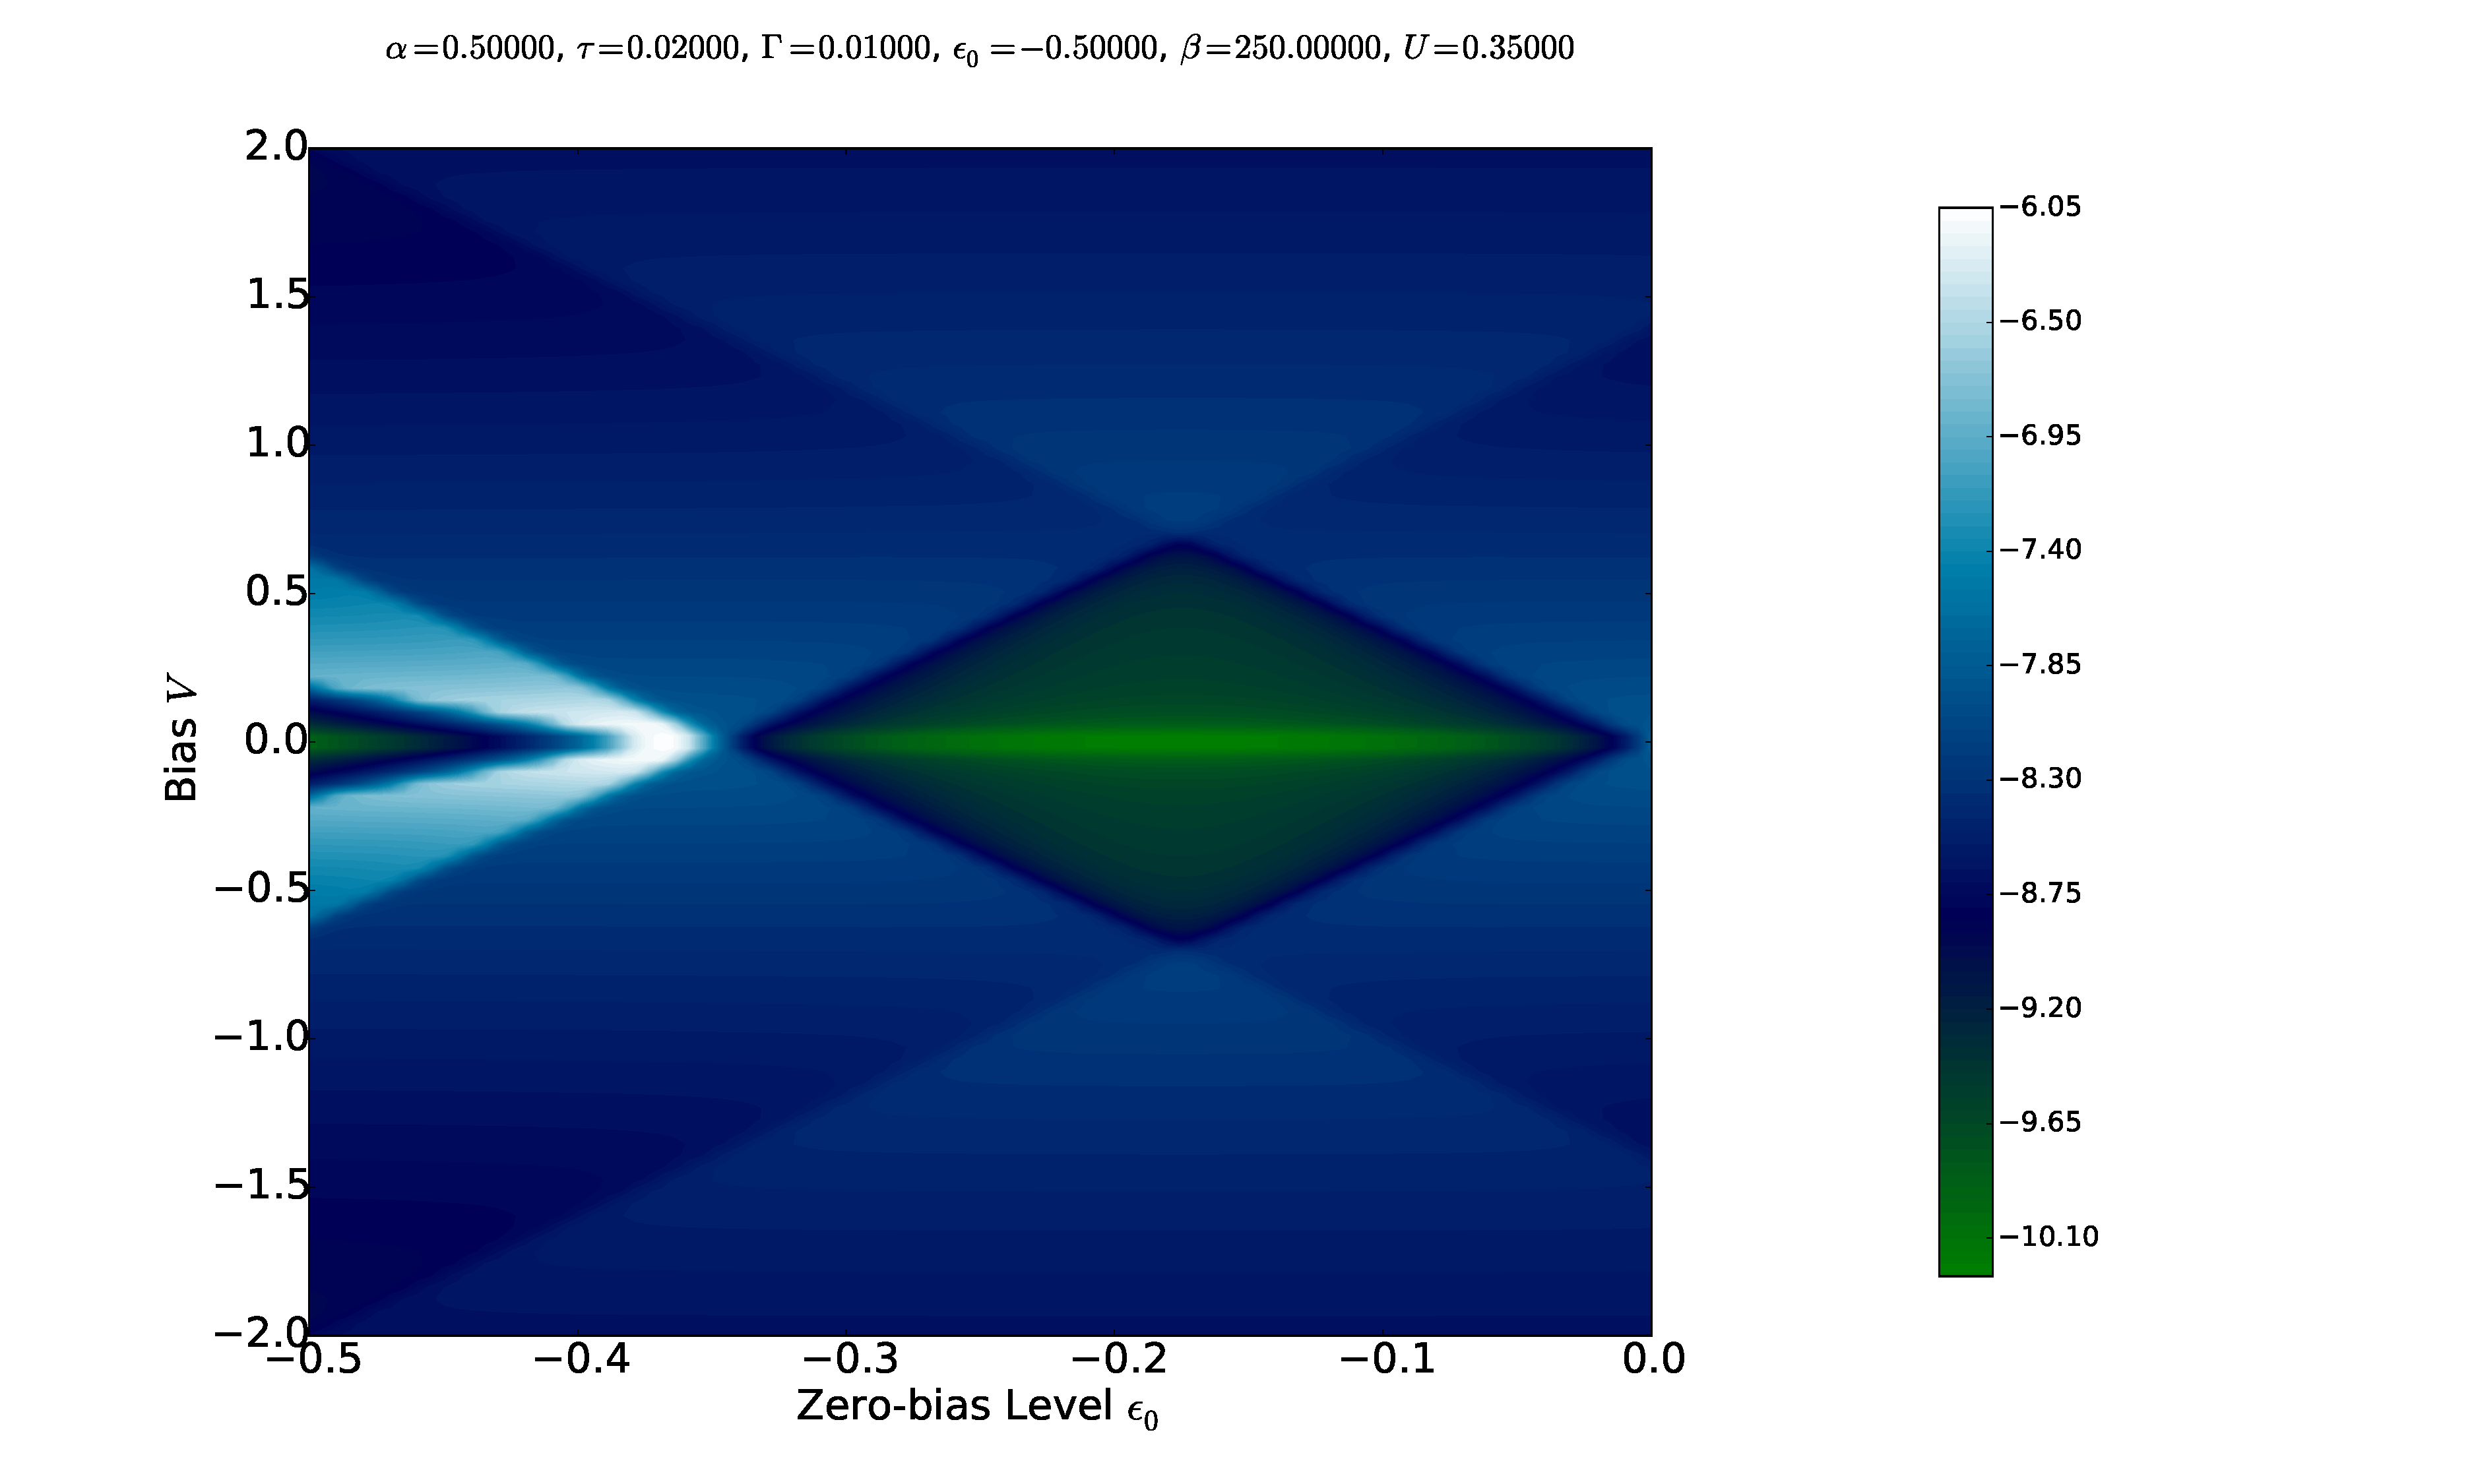
\includegraphics[height=.38\textheight]{pdf/coulombd/current_map_diamond_alpha_05.pdf}
    \caption{In this figure, $U=0.35$ and $\alpha=0.50$. The colours are based on the $^{10}\text{log}\left|I(V)\right|$, so that the NDC is implied because $I(V) = -I(-V)$.}
    \label{fig:diamond50}
\end{figure}
\begin{figure}[htb]
    \centering
    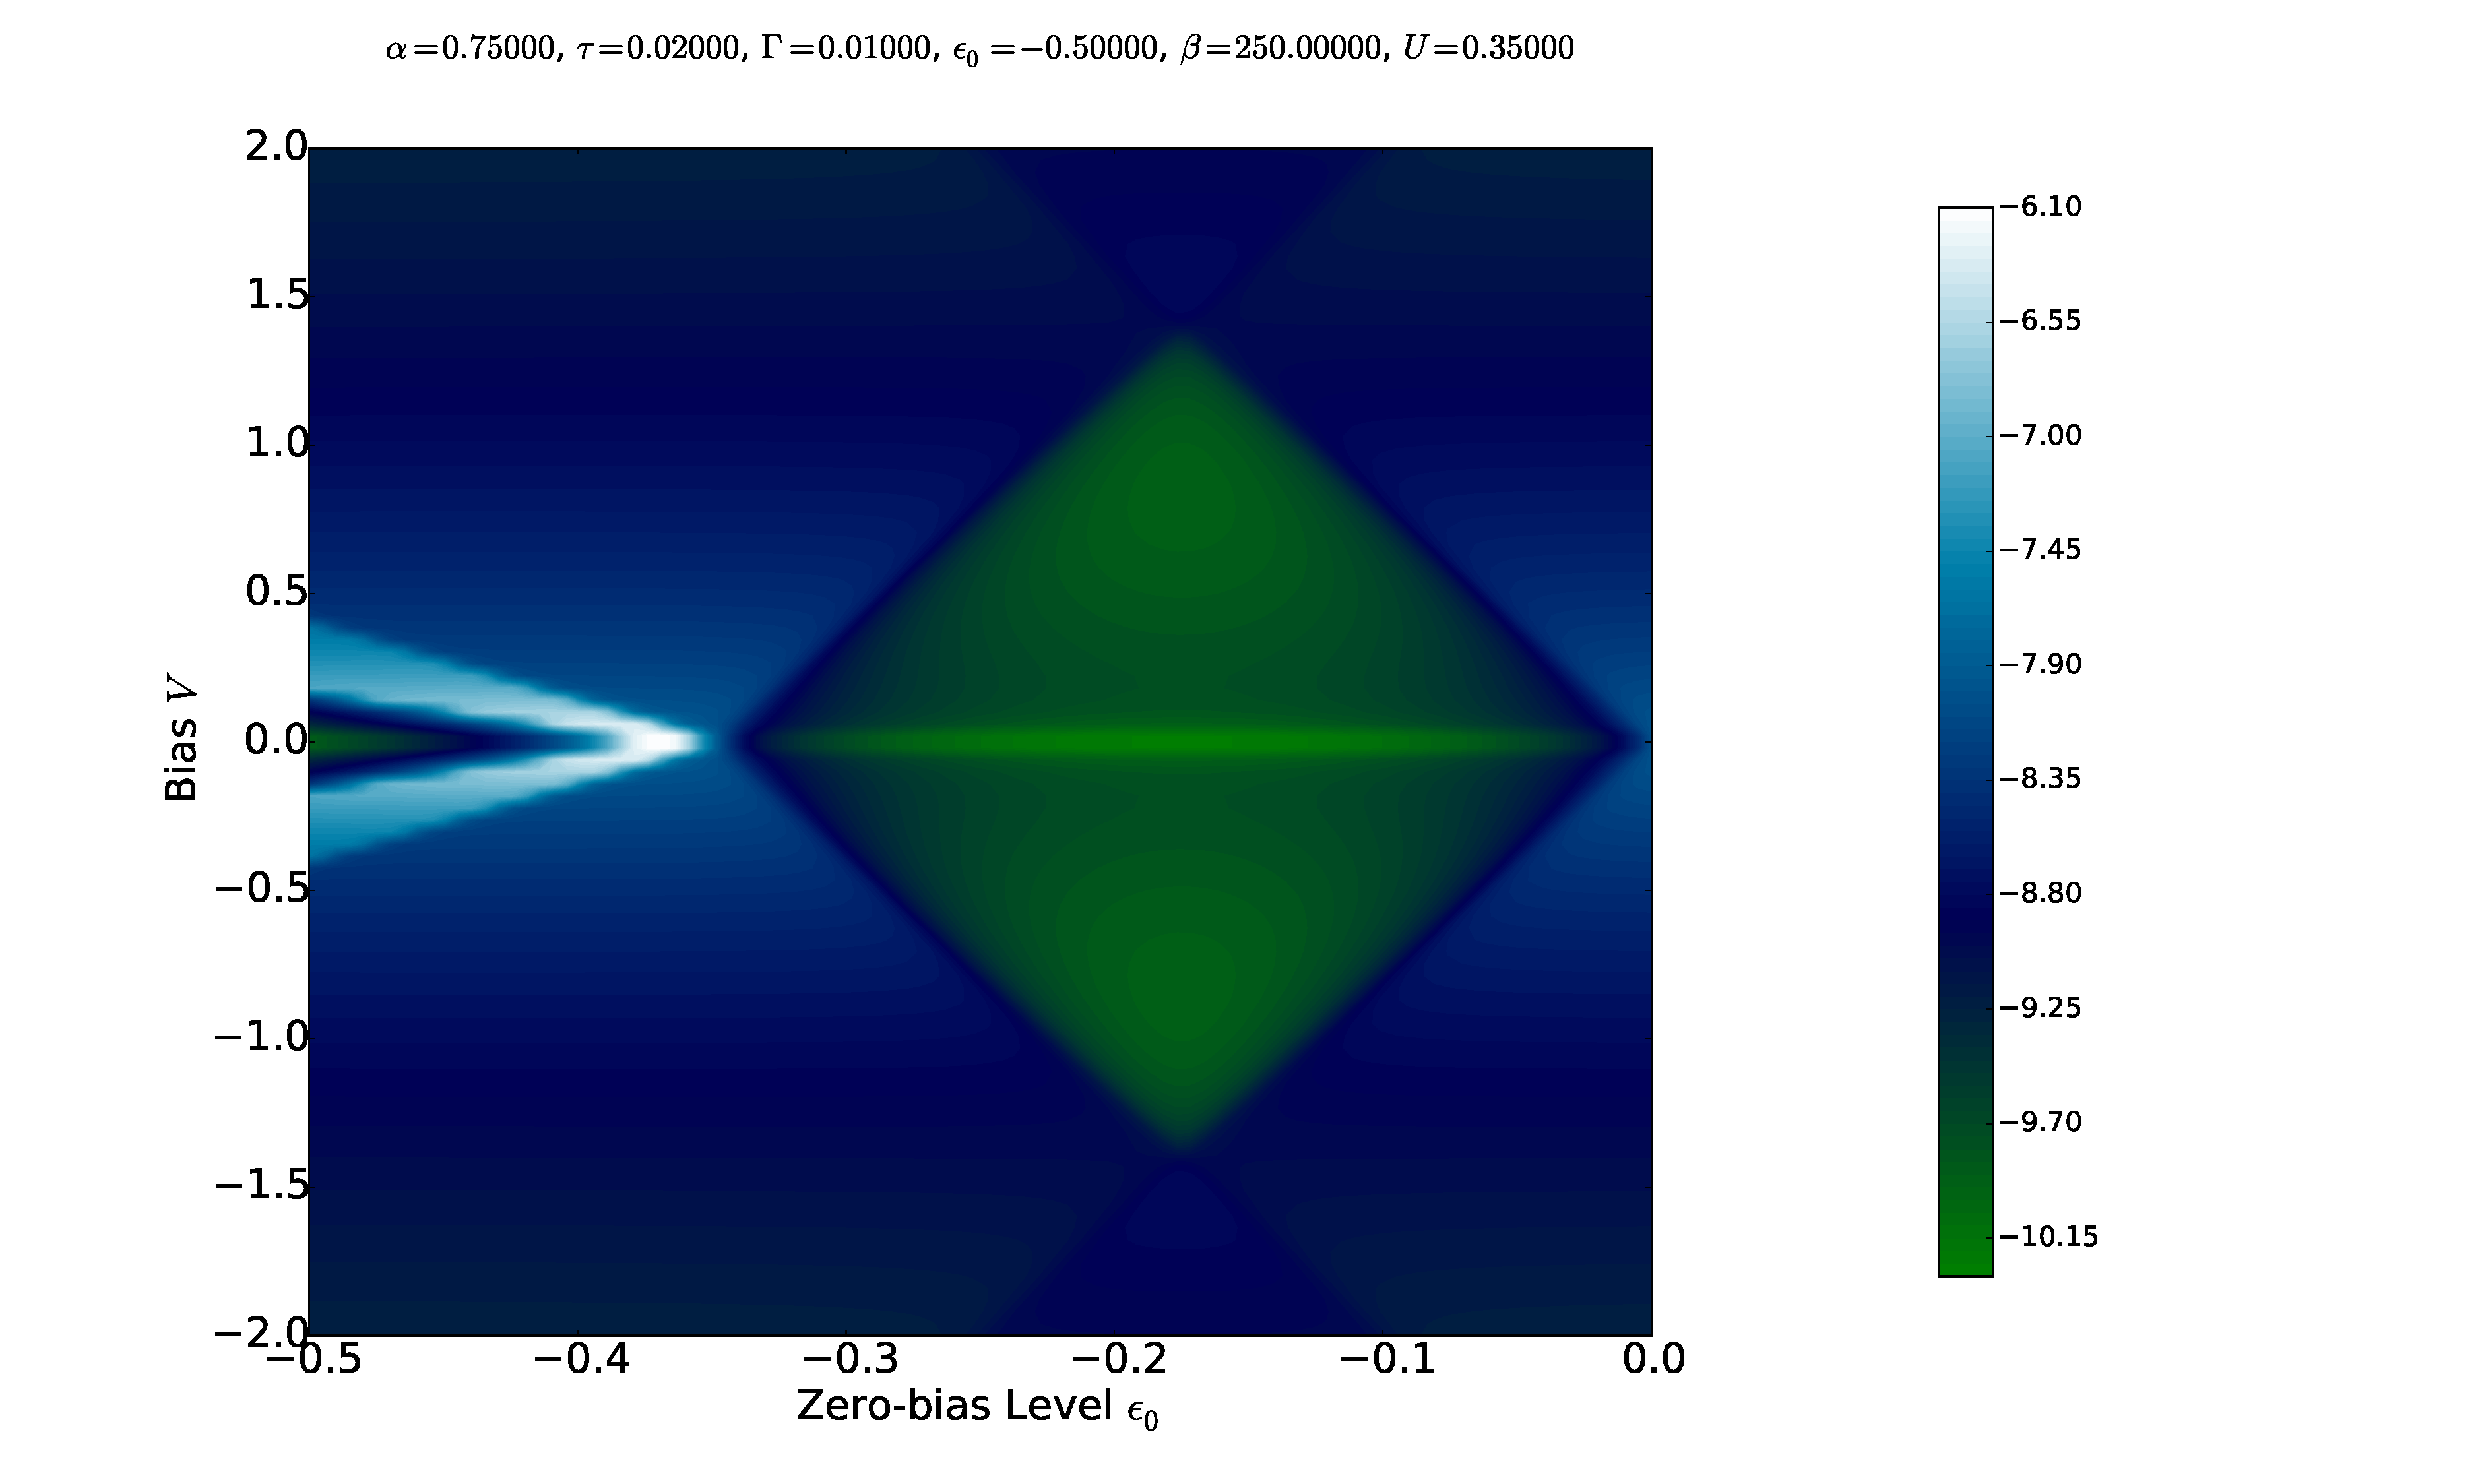
\includegraphics[height=.38\textheight]{pdf/coulombd/current_map_diamond_alpha_075.pdf}
    \caption{In this figure, $U=0.35$ and $\alpha=0.75$. The colours are based on the $^{10}\text{log}\left|I(V)\right|$, so that the NDC is implied because $I(V) = -I(-V)$.}
    \label{fig:diamond75}
\end{figure}

\section{Experimental fit}
\label{sec:perrin}
On inspection of the peak values of current when the many-body occupation is the first charge state, I found that the current was already less than it was in \citet{perrinnano} or the zero-charge state. In Figure~\ref{fig:imax}, I compare the peak current at certain capacitive interaction strength for the edge of the first and second charge states. The first charge state has the left and right sites at different energies, so that current is suppressed relative to the second charge state which has both levels at the same energy.
\begin{figure}[htb]
    \centering
    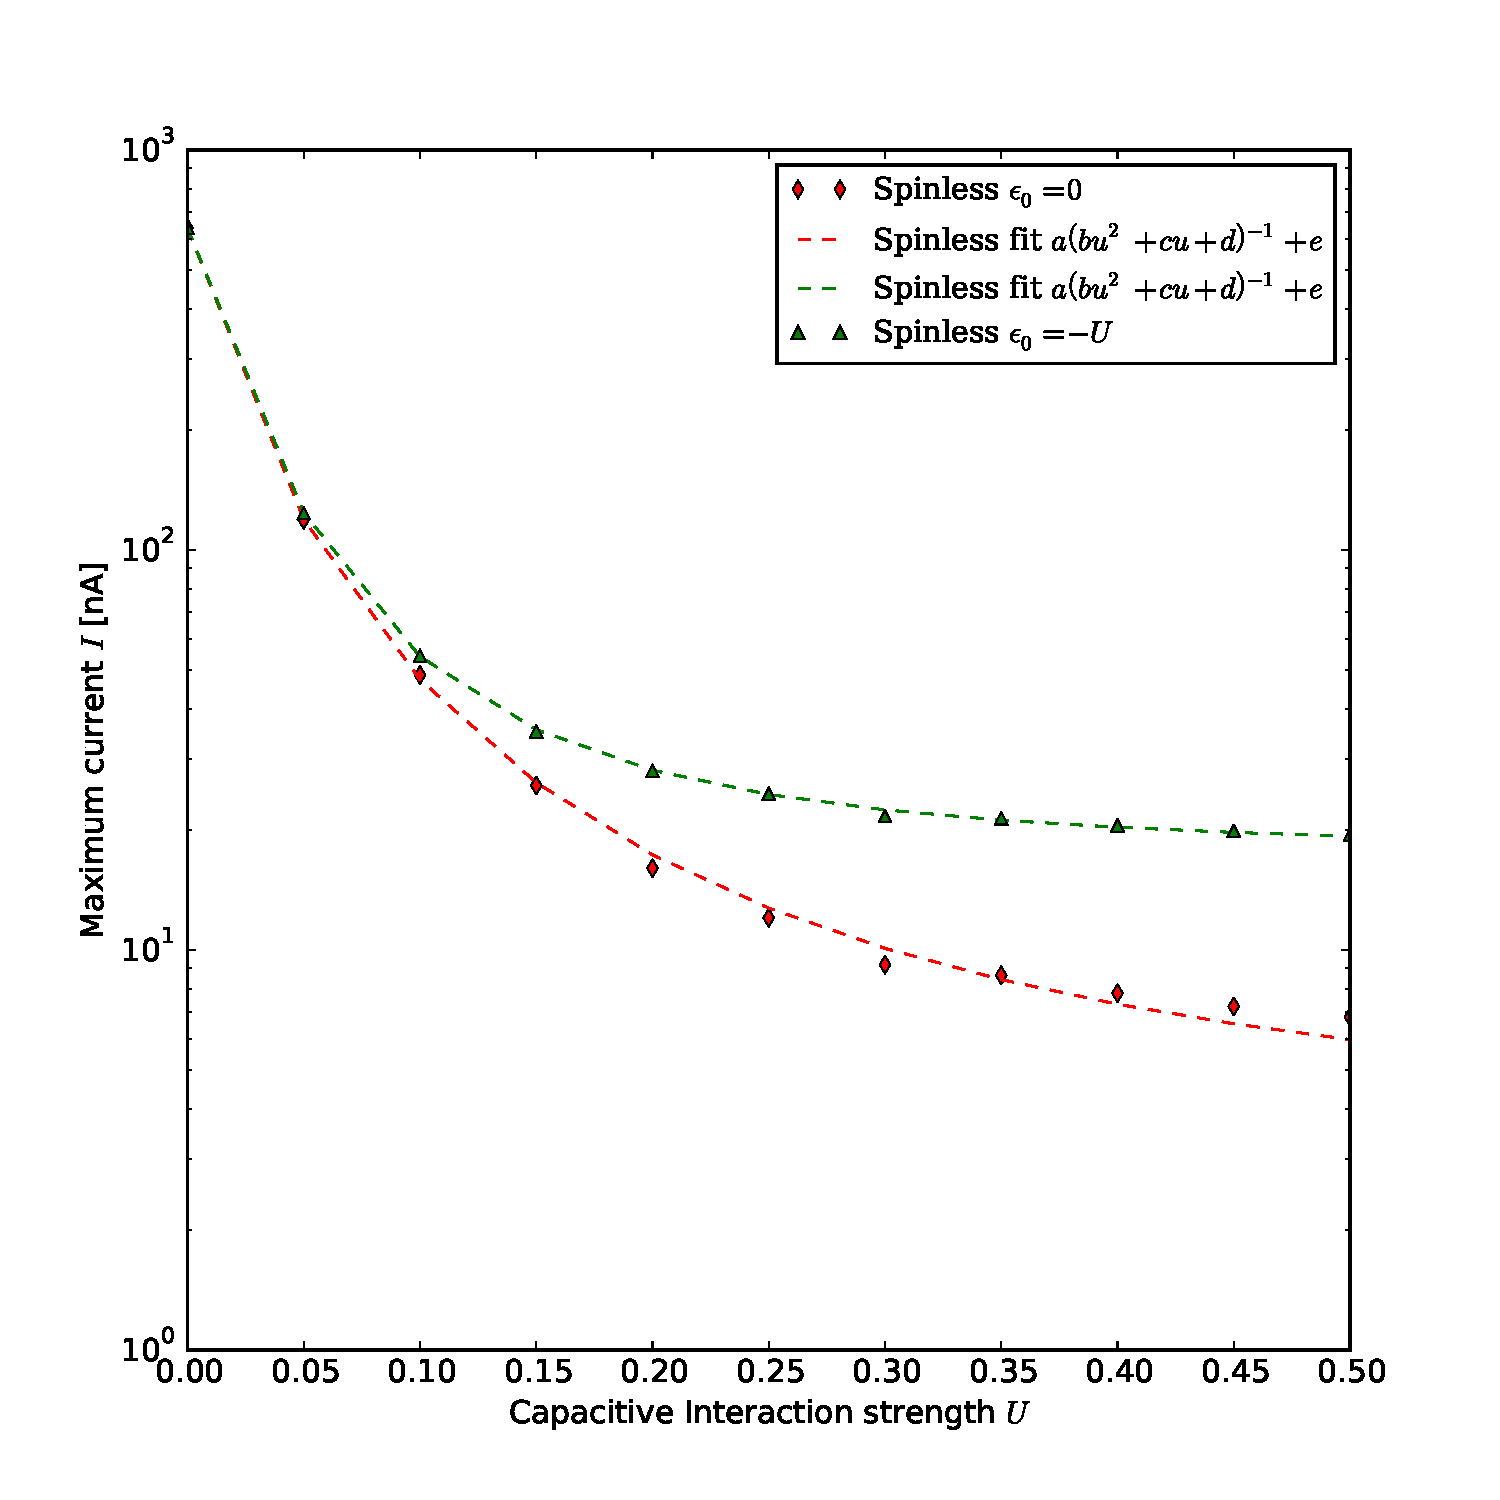
\includegraphics[height=.38\textheight]{pdf/imax.pdf}
    \caption{In this figure, $\alpha=0.50$, $\tau=0.02$, $\Gamma=0.01$, $\epsilon_0 = 0$ or $\epsilon_0=-U$. I show the maximum current versus the capacitive interaction, for the first charge state (red diamonds) and the second charge state (green triangles). Visible is that the second charge state has a current that is within one order of magnitude larger, likely because the left/right levels align. Both sets fit well to a fit to an inverse polynomial of $U$. See main text for explanation.}
    \label{fig:imax}
\end{figure}

Figure~\ref{fig:imax} seems to indicate that the maximum current will flatten out, so that peak currents of approximately $10$ nA in the first charge state and approximately $5$ nA are expected for strong interaction $U \gtrsim 0.30$. This can be understood from the following. In the supplement to Ref.~\cite{perrinnano}, they compute the current for a two-site model in terms of the bonding ($\pi$) and anti-bonding ($\pi$) orbitals. The current is proportional to the inverse of the level splitting, $\left( \Delta^2 + \Gamma^2 \right)$. The level splitting for the interacting case can be found from the eigenvalues of e.g. $\begin{bmatrix} \epsilon_0 + \frac{1}{2} \alpha V+U & -\tau \\
-\tau & \epsilon_0 - \frac{1}{2} \alpha V\end{bmatrix}$:
\begin{align*}
\Delta^2 &= U^2 + U \left(4\epsilon_0 - 2 \alpha V\right) + \alpha^2 V^2 - 4 \tau^2,
\end{align*}
so that the maximum current is proportional to the inverse of a second-order polynomial of $U$. The fits in Figure~\ref{fig:imax} show that this simply analysis yields the correct results. The second charge state is expected to yield a higher current, as $\Delta$ reduces by $4 \left|\epsilon_0 \right| U$. This agrees with the concept that the first charge state has misaligned levels, because that indicates a larger $\Delta$ and thus a lower current, whereas thee second charge state has a small $\Delta$ and a high current. However, I must caution that this analysis and Figure~\ref{fig:imax} concern only non-degenerate states.

These results indicate that the Coulomb interaction energy is in principle able to tune the peak current. Note that the Coulomb interaction energy will at some point induce a switch to a different many-body state (section~\ref{sec:expectations}). I will look at the measurements by Mickael Perrin \cite{perrin, perrinnano}, whom has kindly given me one of his datasets to look at. 

In figure~\ref{fig:perrindata}, a break junction measurement for different separation differences (gap sizes) is shown. As the separation distance increases, the current drops increasingly, until an apparent Coulomb gap opens suddenly around separation $s \approx 663$. As I showed in section~\ref{sec:expectations}, very sudden transmission changes can occur due to many-body state switches. I surmise a similar thing has happened here. As separation distance increases, we see that the $V=0$ flattish area starts increasing. At approximately $s\approx 663$, it suddenly widens and a rather clear Coulomb blockade is visible. While there is no good way to estimate the theoretical parameters from such an experiment, speculation is possible. If all parameters change slowly, then this could simultaneously explain both the peak current dropping and the opening of a flat area in between. For $s \lesssim 663$, the zero charge state is likely occupied, based on the current at $s = 638$ and the smooth change from there. The zero bias level $\epsilon_0$ slowly move off-resonance as separation increases, which is the opening of the plateau. Then, at $s \approx 663$, a many-body switch happens and the molecule is found in the first charge state. As $\epsilon_0 \neq 0 $ and $\epsilon_0 \neq -U$, we are inside the Coulomb diamond of the first charge state. Afterwards, the theme of slowly changing parameters continue and the gap widens. I must point out that in the current sweeps presented here, many-body switches always occurred at the tip of a diamond. However, I do think this speculation has merit all the same.
\begin{figure}[htb]
    \centering
    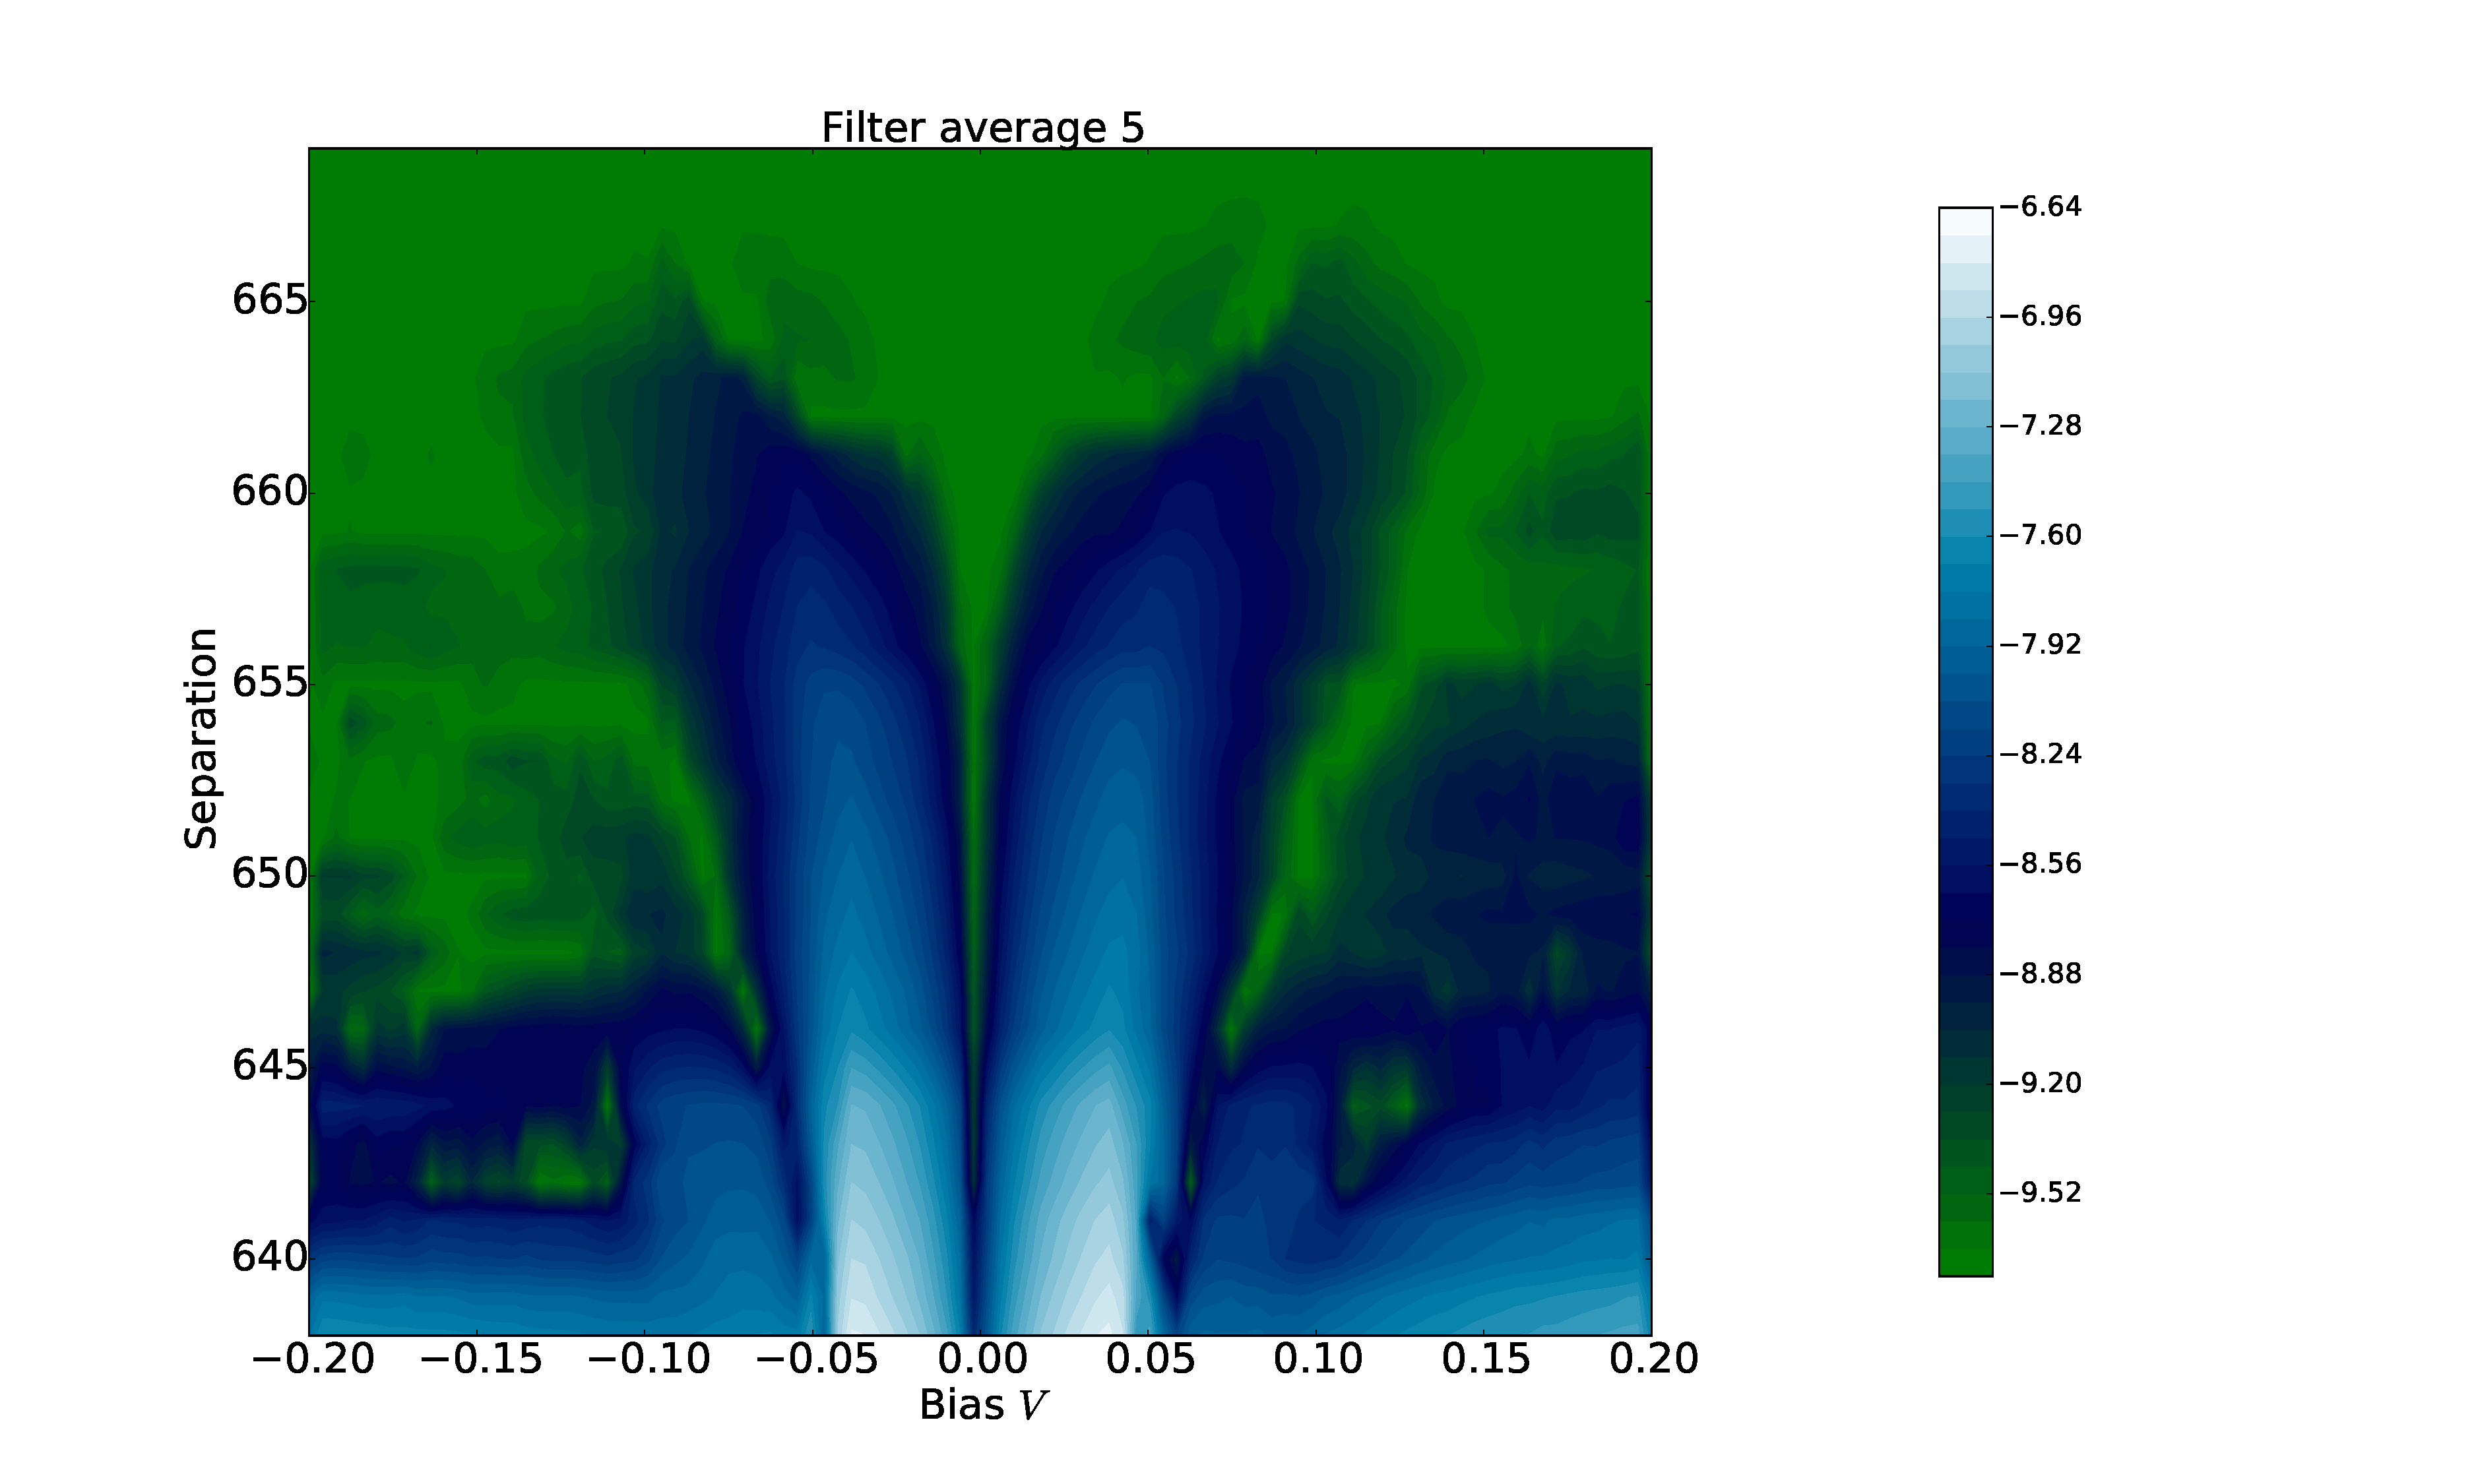
\includegraphics[width=.99\textwidth,clip=true, trim=4cm 0cm 10cm 4cm]{pdf/perrin_experiment_abs.pdf}
    \caption{Experimental data by \citet{perrinnano}, the colours are proportional to $^{10}\text{log}\left|I(V)\right|$. As elsewhere, $I(V) = -I(-V)$. The current is capped at the lower end to $10^{-10}$ A.}
    \label{fig:perrindata}
\end{figure}

Next, I want to presents a few results that show clearly that the new theory is in better quantitative agreement with the results by \citet{perrinnano}. However, the current landscape at different parameters does not change smoothly, which makes it troublesome to \emph{fit} the predicted smoothly. Instead, I performed an automatic rough parameter scan and selected results manually.

In particular, I have taken care to select results both in the first and second charge state, to show that both possibilities are relevant. First, I want to discuss the spinless results and then the spinfull results. For all of these figures, $\alpha=0.400$, $\Gamma=0.010$, $\tau=0.010$ unless otherwise noted. The experimental current is measured in the exact same way as Figure~\ref{fig:perrindata}, but only the (near) blockade-free region was used.

Figure~\ref{fig:fitspinless5} with $U=0.30$ and $\epsilon_0=-0.30$, shows a very clear NDC with maximum current within a factor of two relative to the averaged experimental current, a significant improvement over the previous prefactor $10^-5$ in Ref.~\cite{perrinnano}.


\begin{figure}[htb]
    \centering
    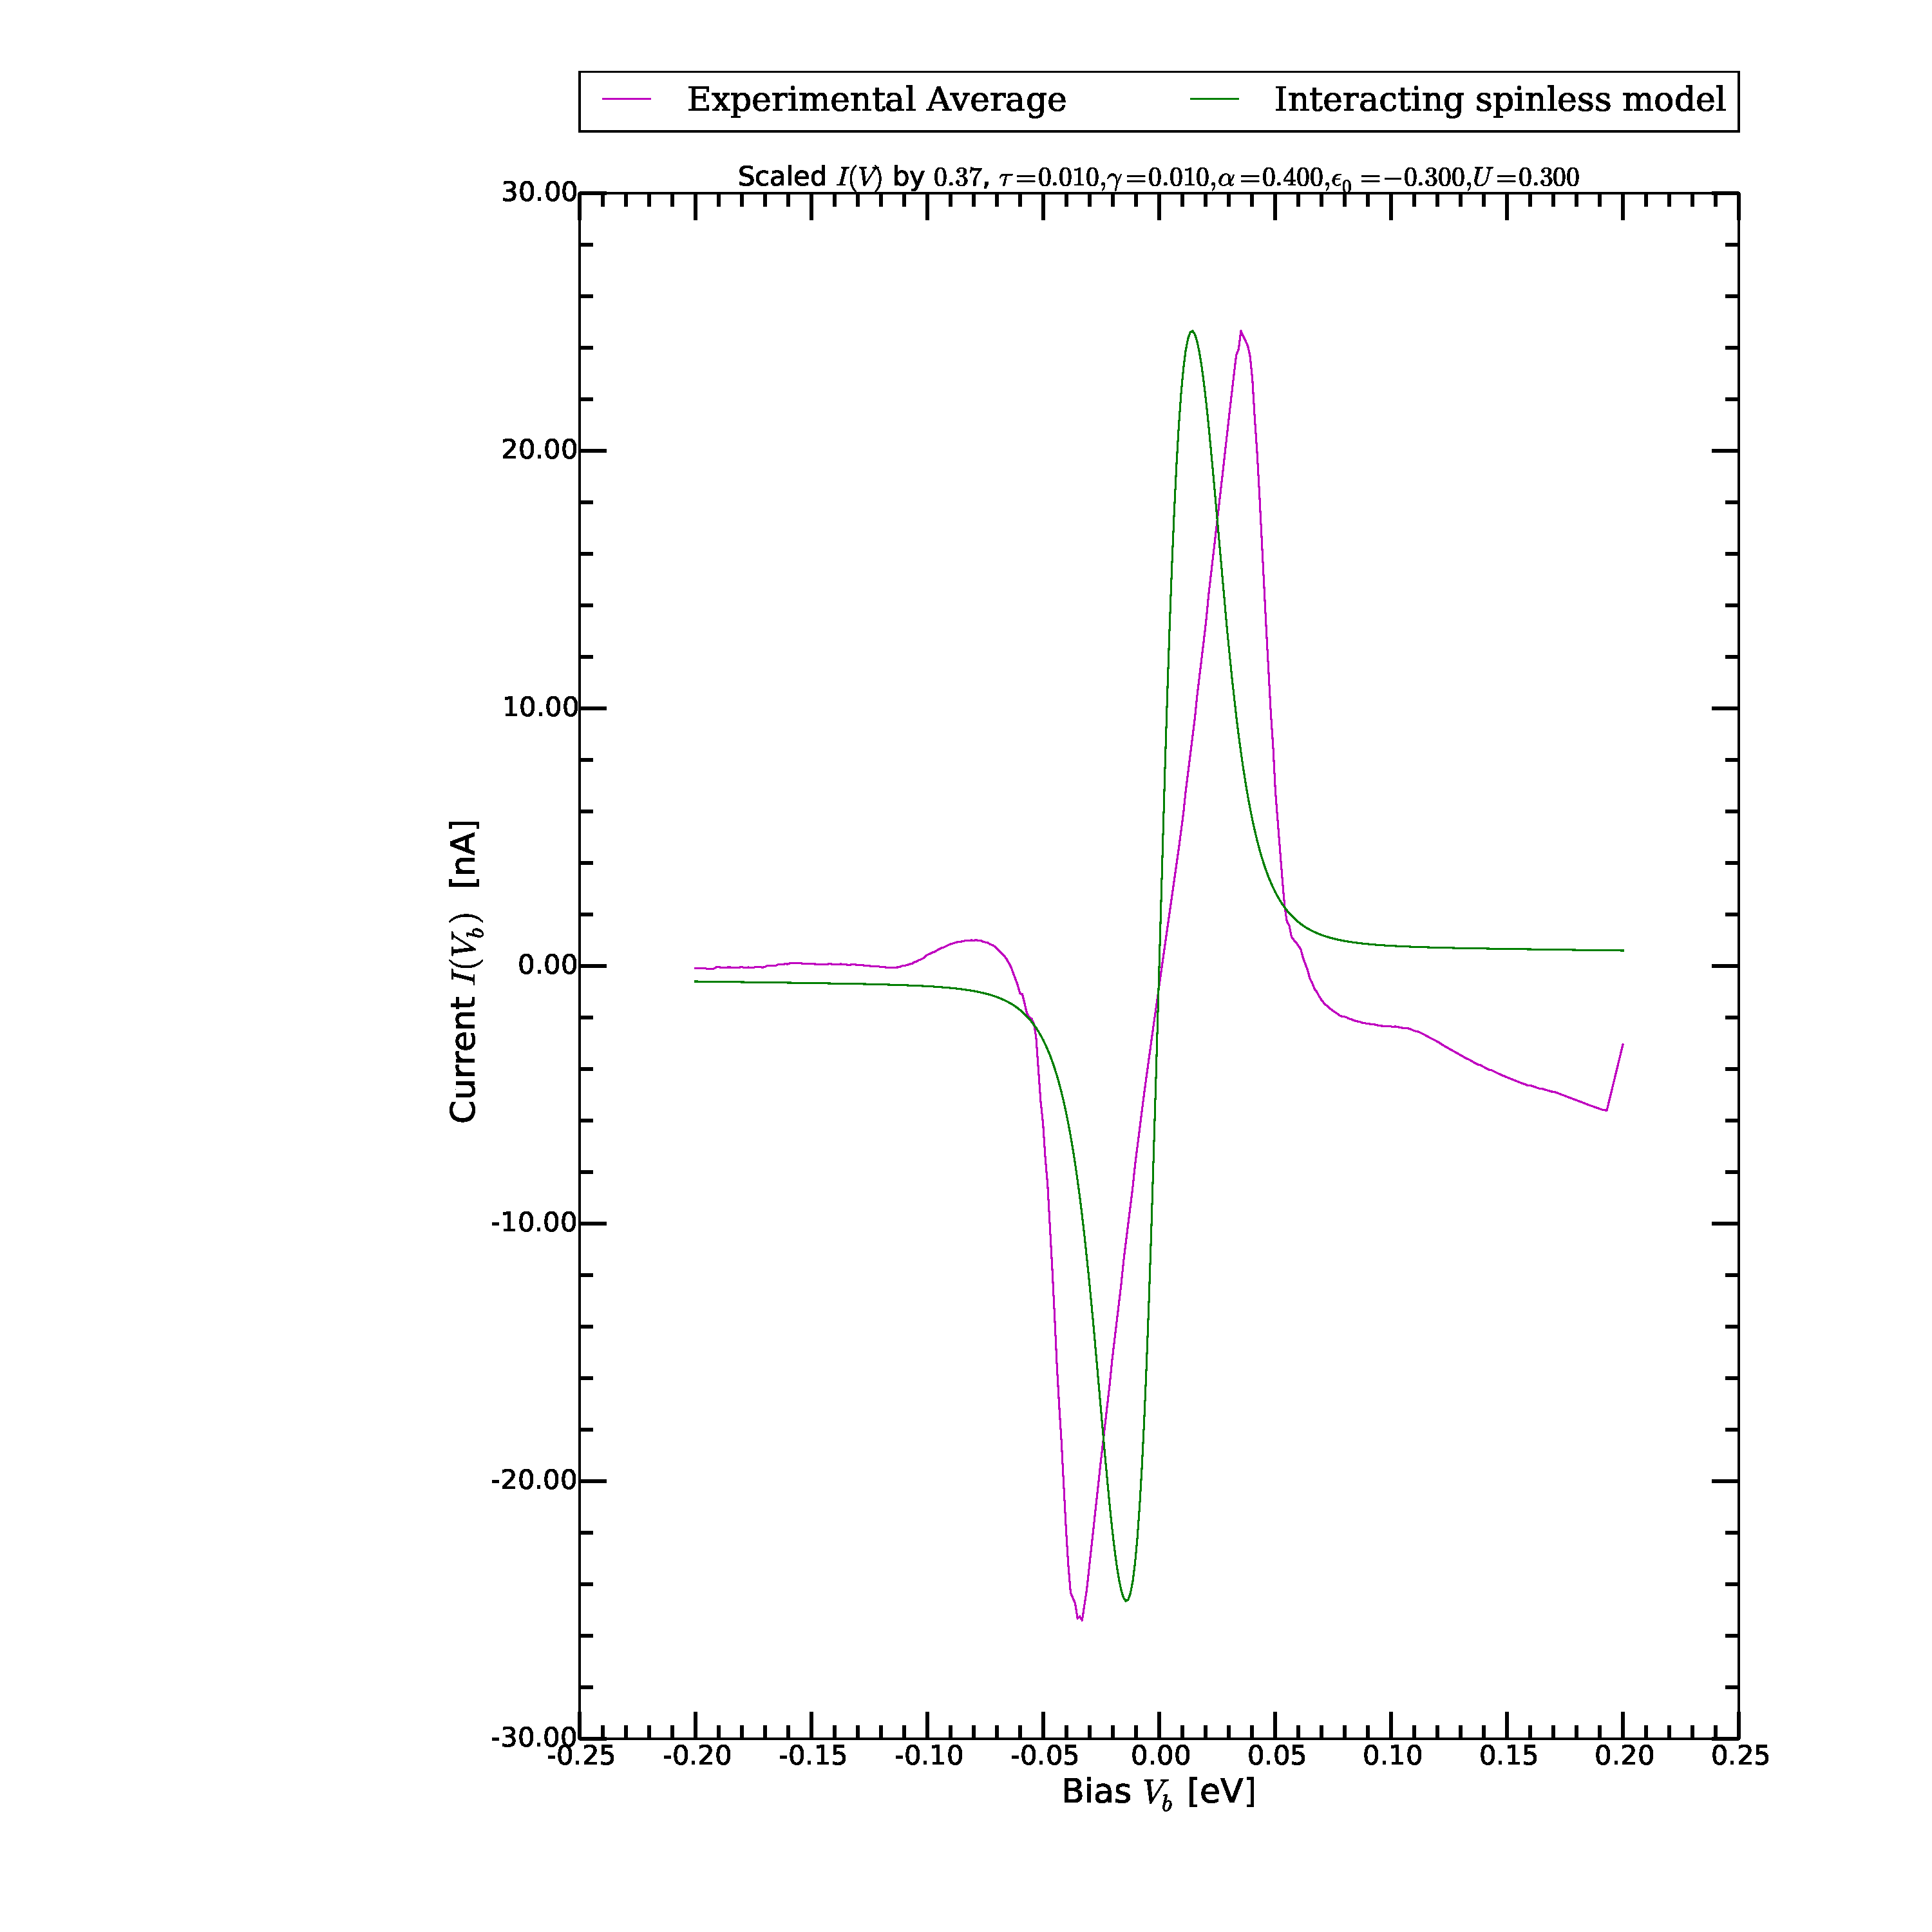
\includegraphics[width=.95\textwidth, clip=true, trim=11cm 2cm 2cm 0cm]{pdf/fit/fit_spinless_5.pdf}
    \caption{Experimental $I(V)$ (Magenta) versus calculated spinless current $I(V)$ (green). In this figure, $U=0.30$ and $\epsilon_0 = -0.30$. The current is scaled by $0.37$ so that it has the same peak height as the experimental current.}
    \label{fig:fitspinless5}
\end{figure} 
\begin{figure}[htb]
    \centering
    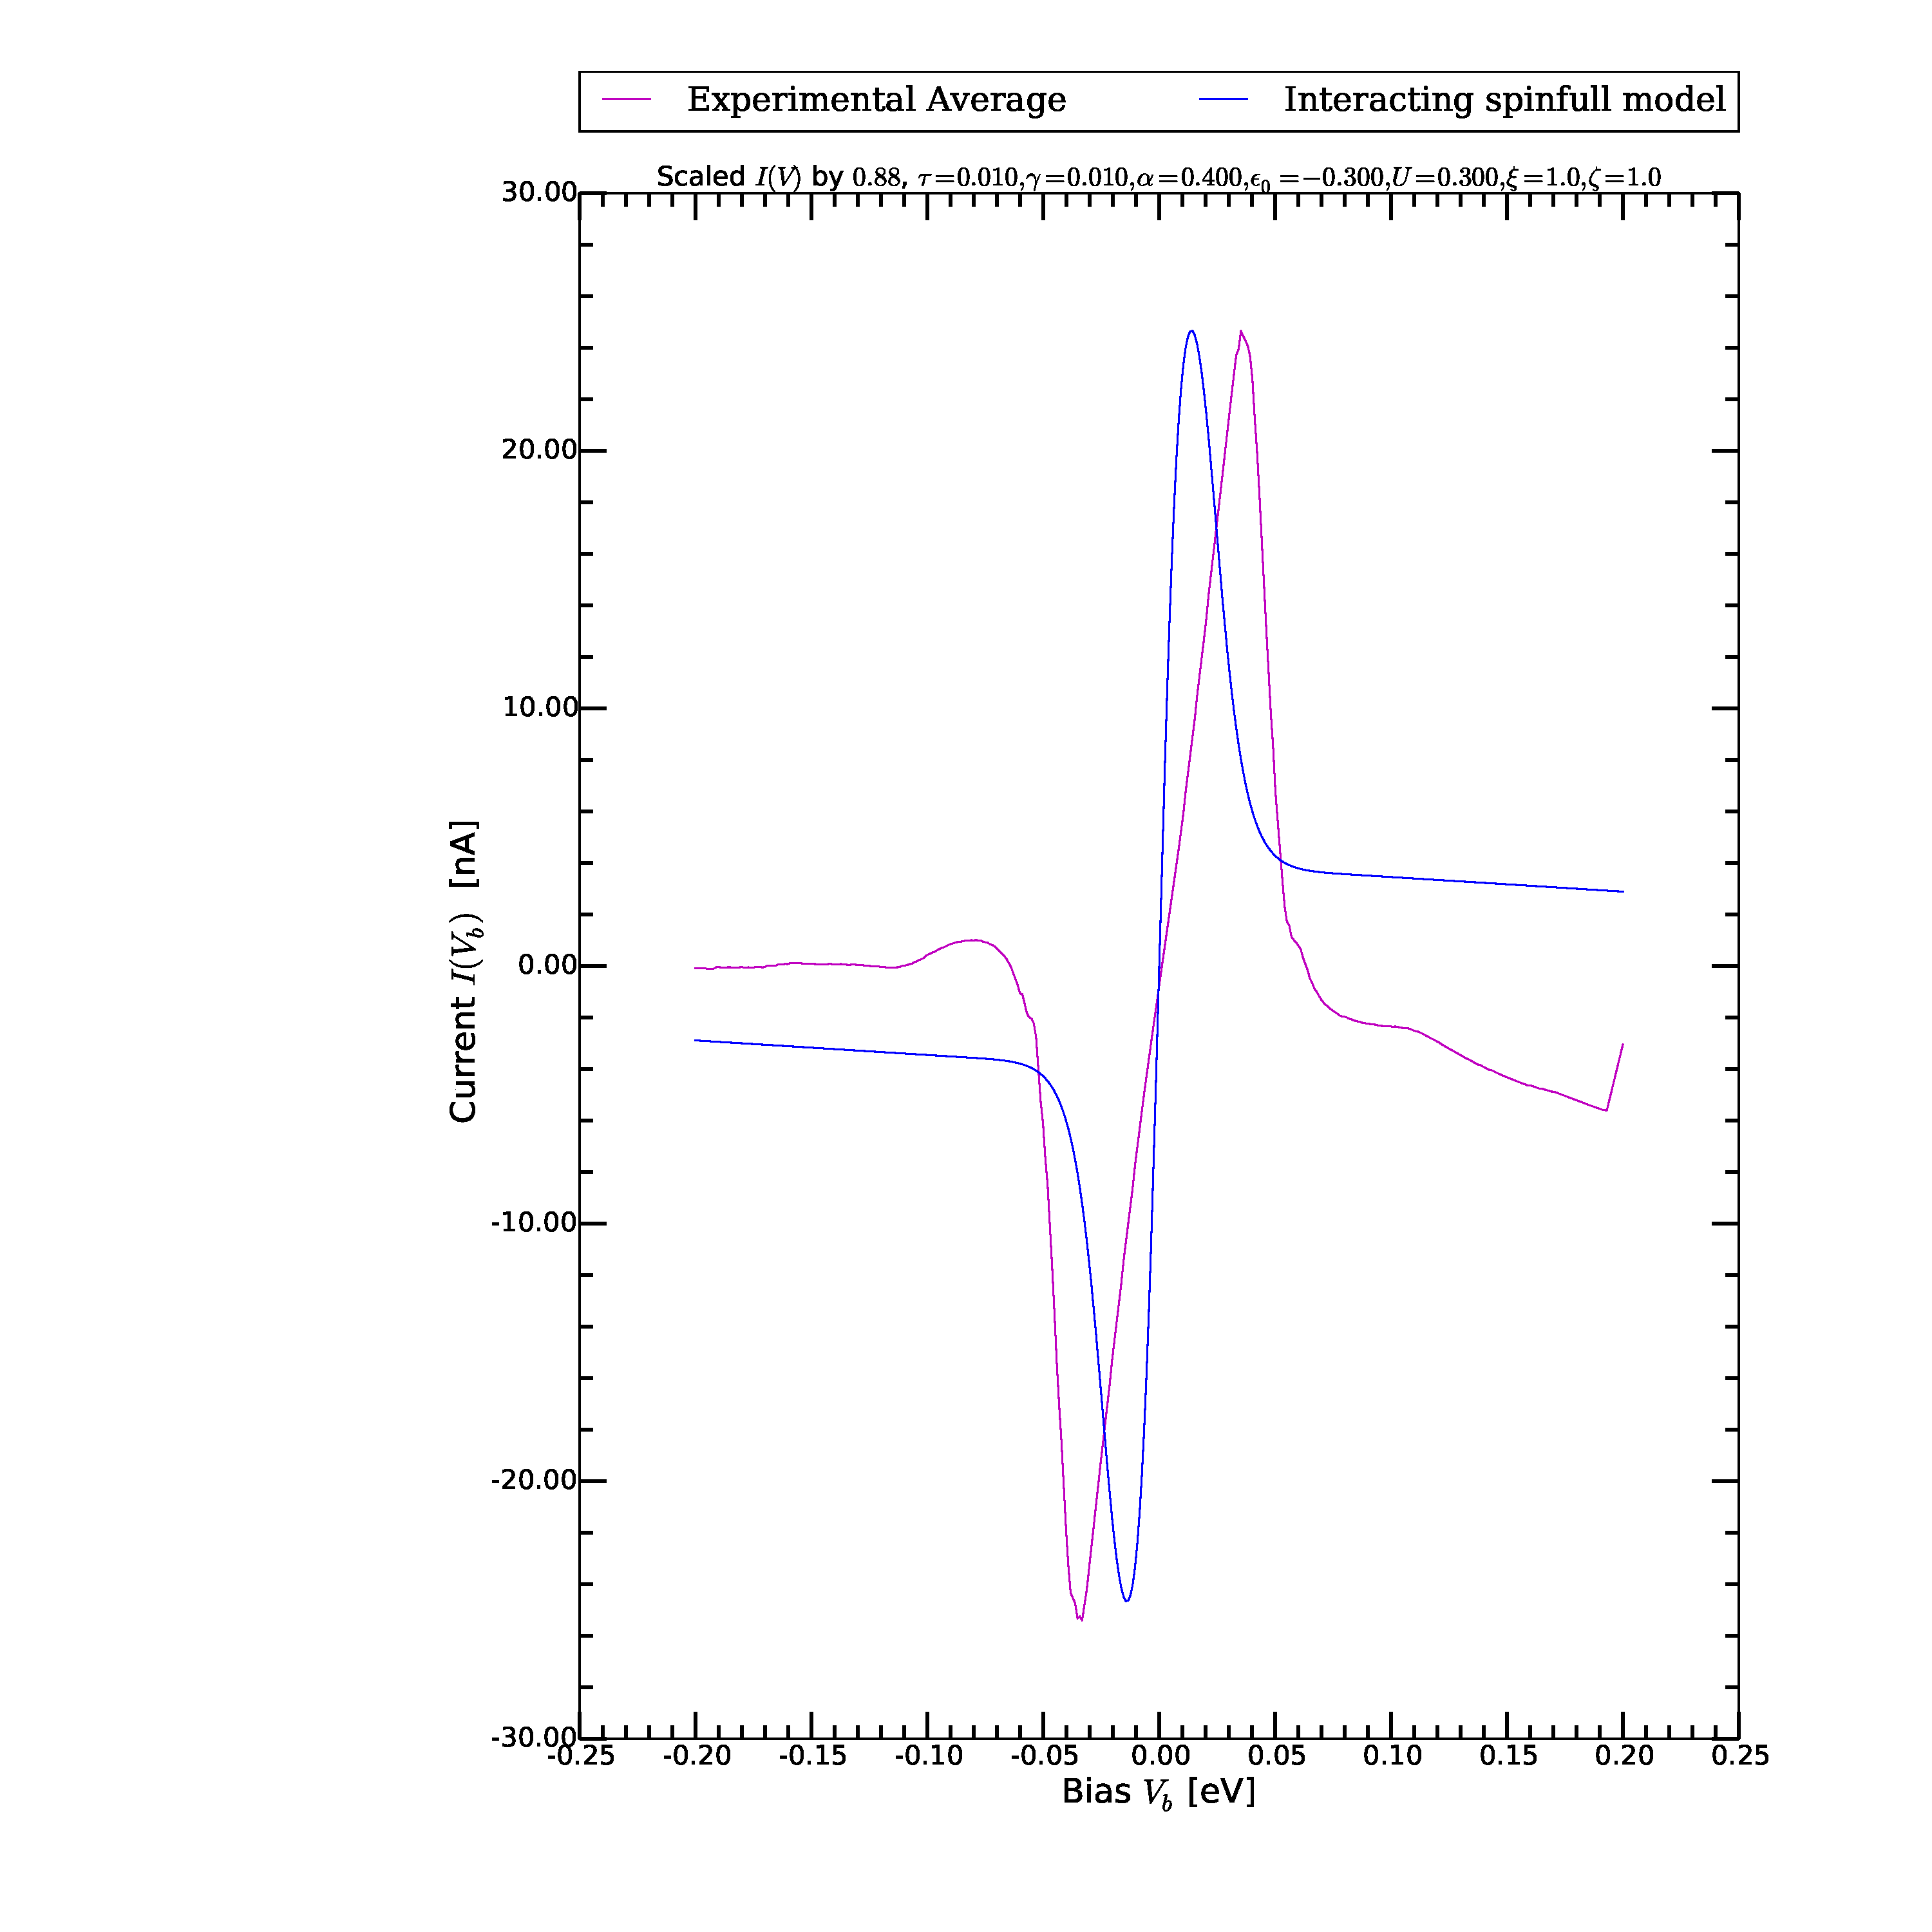
\includegraphics[width=.95\textwidth, clip=true, trim=11cm 2cm 2cm 0cm]{pdf/fit/fit_spinfull_1.pdf}
    \caption{Experimental $I(V)$ (Magenta) versus calculated spinfull current $I(V)$ (green). In this figure, $U=0.30$ and $\epsilon_0 = -0.30$. The current is scaled by $0.88$ so that it has the same peak height as the experimental current.}
    \label{fig:fitspinfull1}
\end{figure} 

The second charge state is shown in Figure~\ref{fig:fitspinfull1}, which does have lower peak current, within a factor 2 of the experimental average. For $U=0.50$, the first charge state is very similar to the second, but is at $169$ \% while the second charge state is at $95$ \% of the experimental average.

To conclude, the quantitative agreement with \citet{perrinnano} is significantly improved in the first and second charge states. While the peak voltages do not exactly agree, we only performed a very limited rough scan of the parameter space. I am confident that the parameters can be tuned for better qualitative agreement, but could not do so due to time-constraints.

\section{Self-Consistent Results}
\label{sec:resultsselfconsistencycalc}

\begin{figure}[htb]
    \centering
    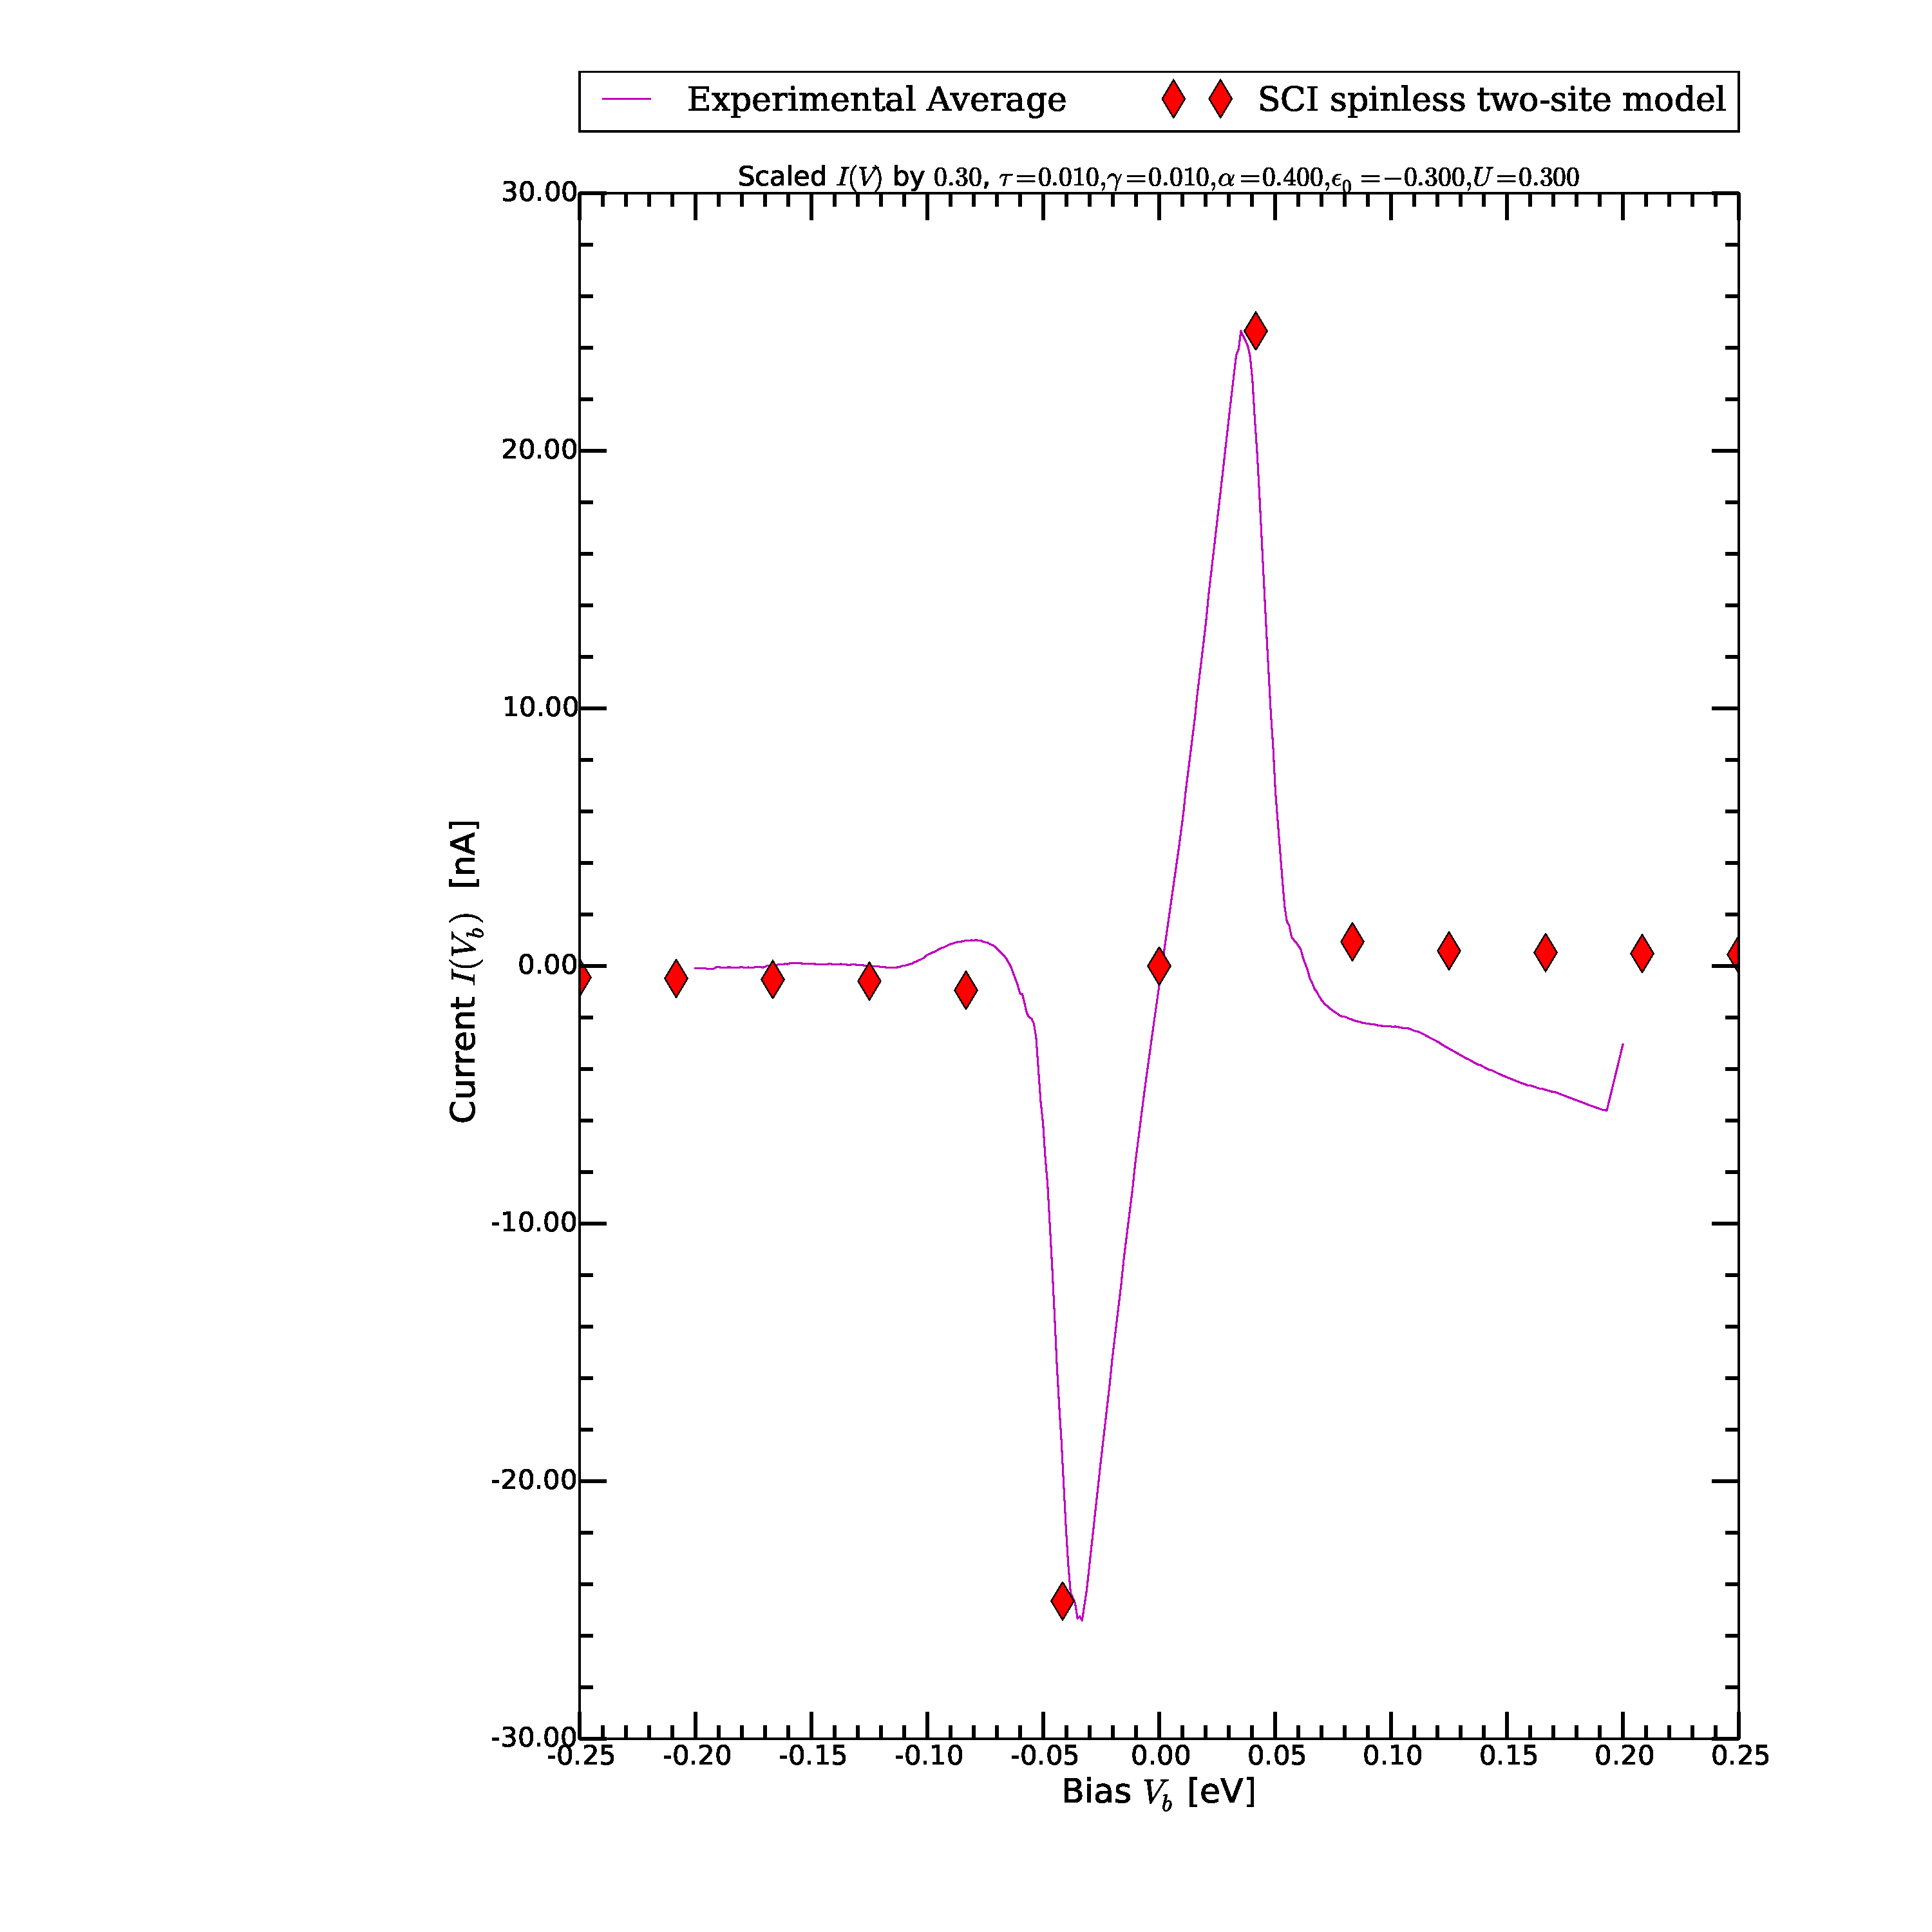
\includegraphics[width=.95\textwidth, clip=true, trim=11cm 2cm 2cm 0cm]{pdf/selfconsistent_fit_current_0.pdf}
    \caption{ }
    \label{fig:figselfconsistent}
\end{figure} 

%clearpage dumps all images in the stack. Also prevents images from skipping chapters.
\clearpage
\references{dissertation}
\chapter{Summary}
\label{ch:chapter_5}

%% The following annotation is customary for chapter which have already been
%% published as a paper.
%\blfootnote{Parts of this chapter have been published in Annalen der Physik \textbf{324}, 289 (1906) \cite{Einstein1906}.}

%% It is only necessary to list the authors if multiple people contributed
%% significantly to the chapter.
%\authors{Albert {\titleshape Einstein}}

%% The '0pt' option ensures that no extra vertical space follows this epigraph,
%% since there is another epigraph after it.
%\epigraph[0pt]{
%    "quote1"
%}{attribution}

%no abstract

%% Start the actual chapter on a new page.
\newpage
\section{Introduction}
Most theses do not accurately depict all of the work performed. Rather, it depicts the successful work and does not mention the failures. For instance, we were quite excited about a region of apparent resonance within the Coulomb diamond, only to find out that this a plotting artifact in those pictures. Perhaps one of the greater possible improvements in science would the a journal called "The international journal of complete blunders". A great amount of resources is spent in futility, simply because scientists do not often communicate what did not work.

Even so, I think it is fair to say that the results as presented here are fairly consistent with intuition, theory and experiment. It gives a reasonable impression of the work done, both in derivation as in finding meaningful results in the two-site model. 

I have presented the main results, which I will summarise in section~\ref{sec:summary}. I then discuss the results and the implications of my thesis in section~\ref{sec:discussion}. Finally, I provide an outlook in section~\ref{sec:outlook}.


\section{Summary}
\label{sec:summary}
A brief overview of the experimental and theoretical status of the field was provided in chapter~\ref{ch:chapter_1}. In this chapter I listed a few of the experimental difficulties, outlined the ME approach and the difficulty of treating capacitive interaction.

A derivation of the non-equilibrium Green's Function Formalism was presented in chapter~\ref{ch:chapter_2}. I started with the Dyson equation (equation~\ref{eq:dyson}) and we used the Langreth rules to derive the Keldysh equation (equation~\ref{eq:keldysh}). The equation of motion (EOM) method for finding the exact shape of the Green's functions was demonstrated. I then showed how to calculate the spectral density, and more importantly the current by means of the Landauer equation (equation~\ref{eq:landauer}). I concluded that chapter by a short summary (section~\ref{sec:synthesis}).

In chapter~\ref{ch:chapter_3}, I looked at interactions and how to incorporate them to the non\hyp{}equilibrium Green's Function Formalism. In particular, I looked at electron-electron capacitive interaction and I presented Dr. Jos Seldenthuis his derivation of the capacitive self-energy and the resulting many-body Green's Function $\mathscr{G}^\kappa$. I then provided an alternative, simpler derivation of its expectation value.Noting the difficulty in finding the form of the non-equilibrium density matrix, I presented a derivation for a self-consistent scheme to find the non-equilibrium density matrix. As it turned out, the expectation value approach for the many-body Green's function was also useful in deriving an elaborate expression for the incorporation of interaction with a single bosonic level (vibrations, phonons). 

I then showed the explicit form of the capacitive-self energy for a two-site model, both with and without spin, in chapter~\ref{ch:chapter_4}. I briefly considered the self-consistent density matrix, but applied the equilibrium density matrix approximation throughout most results. I then presented results for the transmission which showed direct evidence of the many-body behaviour in our model. Next, I presented stability diagrams and explored the properties of the resulting Coulomb Diamonds. 

Finally, I revisited the experiment of Ref.~\cite{perrinnano}. The quantitative agreement was shown to have significantly improved. A brief look at a self-consistent $I(V)$ indicated that the self-consistent calculation can also improve the qualitative agreement.

\section{Discussion}
\label{sec:discussion}
Incorporating the capacitive interaction in the non-equilibrium Green's Function Formalism led to very clear Coulomb diamonds, which have been observed in experiments very often. Usually, these discussed in terms of charging effects \cite{seldenthuis, thijszantrev}, although simple systems have been discussed within the non-equilibrium Green's Function formalism \cite{haugjauho}. However, the derivation presented in this thesis includes capacitive interactions into the non-equilibrium Green's Function formalism analytically.

However, such many-body effects depend on the non-equilibrium density matrix, which is usually troublesome to find. I presented a self-consistent scheme to find the non-equilibrium density matrix, although I could not consistently use this approach due to time-constraints. 

The quantitative agreement of the new results with Ref.~\cite{perrinnano} is excellent for the parameters suggest by DFT calculations performed by Jose Celis Gil.  Both parameter-tuning and the self-consistent approach should lead to better qualitative agreement, which should conclude the theoretical analysis of the AH molecule.

\section{Future Outlook}
\label{sec:outlook}
A continuation of my thesis would be to investigate OPE3 \cite{frisenda}, which does not obey a simple toy-model as I presented here. However, as I pointed out for equation~\ref{eq:result}, the expression includes the effective single-particle Hamiltonian $H^\kappa = \mu^\kappa + \tau$ in a specific charge state $\ket{\kappa}$, which can be obtained from DFT calculations. Such an investigation would be very interesting, showing a novel direct application of DFT Hamiltonians within the non-equilibrium Green's Function formalism. Likewise, his findings suggest that the non-equilibrium density matrix will be extremely important, so that treatment of the OPE3 molecule includes both the many-body Green's function and the self-consistent approach for the non-equilibrium density matrix nicely.

With the plethora of molecules available for experiments, there is no doubt that toy-model treatments such as I performed or treatments similar to that suggested above for OPE3 will be very relevant.


%clearpage dumps all images in the stack. Also prevents images from skipping chapters.
\clearpage
\references{dissertation}

%% Use letters for the chapter numbers of the appendices.
\appendix

%\include{appendix-a/appendix-a}

%% Turn off thumb indices for unnumbered chapters.
%\thumbfalse

%\chapter*{Summary}
\addcontentsline{toc}{chapter}{Summary}
\setheader{Summary}

Summary in English\ldots

\chapter*{Samenvatting}
\addcontentsline{toc}{chapter}{Samenvatting}
\setheader{Samenvatting}

{\selectlanguage{dutch}

Samenvatting in het Nederlands\ldots

}


%\chapter*{Curriculum Vit\ae}
\addcontentsline{toc}{chapter}{Curriculum Vit\ae}
\setheader{Curriculum Vit\ae}

%% Print the full name of the author.
\makeatletter
\authors{\@firstname\ {\titleshape\@lastname}}
\makeatother

\noindent
\begin{tabular}{p{4\parindent}l}
    14-03-1879 & Born in Ulm, Germany.
\end{tabular}

\section*{Education}

\begin{tabular}{p{4\parindent}l}
    1892--1896 & Grammar School \\
    & Luitpold Gymnasium, M\"unich (1892--1895)\\
    & Aurau, Switzerland (1895--1896) \\
    \\
    1896--1900 & Undergraduate in Mathematics \& Physics \\
    & Eidgen\"ossische Polytechnische Schule Z\"urich \\
    \\
    1905 & PhD.\ Physics \\
    & Eidgen\"ossische Polytechnische Schule Z\"urich \\
    &
    %% The width of the second column is the width of the page, minus the width
    %% of the first column (4\parindent) minus four times the separation between
    %% the start of the column and its contents.
    \begin{minipage}{\textwidth-4\parindent-4\tabcolsep}
        %% We divide the minipage 20/80.
        \begin{tabular}{@{}p{0.2\linewidth}@{}p{0.8\linewidth-\tabcolsep}}
            \textit{Thesis:} & Eine neue Bestimmung der Molek\"uldimensionen \\
            \textit{Promotor:} & Prof.\ dr.\ A.\ Kleiner
        \end{tabular}
    \end{minipage}
\end{tabular}

\section*{Awards}

\begin{tabular}{p{4\parindent}l}
    1922 & Nobel Prize in Physics \\
    \\
    1925 & Copley Medal \\
    \\
    1929 & Max Planck Medal \\
    \\
    1999 & Time magazine's person of the century
\end{tabular}


%\chapter*{List of Publications}
\addcontentsline{toc}{chapter}{List of Publications}
\setheader{List of Publications}
\label{publications}

%% We use the 'etaremune' environment (the reverse of 'enumerate') to get a
%% numbered list of publications in reverse chronological order. If the list of
%% authors is long, it might be useful to emphasize your own name with \textbf.
\begin{etaremune}{\small

\item \textbf{A.\ Einstein}, \textit{Ist die Tr\"agheit eines K\"orpers von seinem Energieinhalt abh\"angig?}, \href{http://dx.doi.org/10.1002/andp.19053231314}{Annalen der Physik \textbf{18}, 639 (1906)}.
\item \textbf{A.\ Einstein}, \textit{Zur Elektrodynamik bewegter K\"orper}, \href{http://dx.doi.org/10.1002/andp.19053221004}{Annalen der Physik \textbf{17}, 891 (1905)}.
\item \textbf{A.\ Einstein}, \textit{\"Uber die von der molekularkinetischen Theorie der W\"arme geforderte Bewegung von in ruhenden Fl\"ussigkeiten suspendierten Teilchen}, \href{http://dx.doi.org/10.1002/andp.19053220806}{Annalen der Physik \textbf{17}, 549 (1905)}.
\item \textbf{A.\ Einstein}, \textit{\"Uber einen die Erzeugung und Verwandlung des Lichtes betreffenden heuristischen Gesichtspunkt}, \href{http://dx.doi.org/10.1002/andp.19053220806}{Annalen der Physik \textbf{17}, 132 (1905)}.

}\end{etaremune}


\end{document}

